\documentclass[11pt,a4paper,titlepage,final]{article}
\usepackage[utf8]{inputenc}
\usepackage[greek]{babel}
\usepackage{amsmath}
\usepackage{amsfonts}
\usepackage{amssymb}
\usepackage{commath}
\usepackage{xcolor}
\usepackage{hyperref}
\usepackage[skins,theorems]{tcolorbox}
\usepackage{titlesec}
\usepackage{circuitikz}
\usepackage{pgfplots}
\usepackage{gfsartemisia}
\usepackage{mathtools}
\usepackage[makeroom]{cancel}
\usepackage{mathrsfs}
\usepackage{wrapfig}
\usepackage{subcaption}
\usepackage{floatrow}

\usetikzlibrary{arrows.meta}
\usetikzlibrary{patterns}
\usetikzlibrary{decorations.pathmorphing,patterns}
\usetikzlibrary{decorations.markings}
\usetikzlibrary{backgrounds}

\usepackage[left=2cm,right=2cm,top=2cm,bottom=2cm]{geometry}

\makeatletter
%\newcommand{\attnboxed}[1]{\textcolor{red}{\fbox{\normalcolor\m@th$\displaystyle#1$}}}
\makeatother
\tcbset{highlight math style={enhanced,colframe=red,colback=white,%
  arc=0pt,boxrule=1pt,shrink tight,boxsep=1.5mm,extrude by=0.5mm}}
\newcommand{\attnboxed}[1]{\tcbhighmath[colback=red!5!white,drop fuzzy shadow,arc=0mm]{#1}}
\titleformat{\section}{\bf\Large}{Κεφάλαιο \thesection}{1em}{}
\newtcolorbox{attnbox}[1]{colback=red!5!white,%
  colframe=red!75!black,fonttitle=\bfseries,title=#1}
\newtcolorbox{infobox}[1]{colback=blue!5!white,%
  colframe=blue!75!black,fonttitle=\bfseries,title=#1}
  
%\pgfplotsset{compat=1.12}

\title{Σημειώσεις Διαφορικές Εξισώσεις}
\date{2016, Εαρινό εξάμηνο}
\author{\textlatin{\url{https://github.com/kongr45gpen/ece-notes}}}


\newtcbtheorem[number within=section]{theorem}{Θεώρημα}%
{colback=green!5,colframe=green!35!black,colbacktitle=green!35!black,fonttitle=\bfseries,enhanced,attach boxed title to top left={yshift=-2mm,xshift=-2mm}}{th}
\newtcbtheorem[number within=section]{defn}{Ορισμός}%
{colback=cyan!5,colframe=cyan!35!black,colbacktitle=cyan!35!black,fonttitle=\bfseries,enhanced,attach boxed title to top left={yshift=-2mm,xshift=-2mm}}{def}
\newtcbtheorem[number within=section]{exercise}{Άσκηση}%
{colback=gray!3,colframe=gray!35!black,colbacktitle=gray!35!black,fonttitle=\bfseries,enhanced,attach boxed title to top left={yshift=-2mm,xshift=-2mm}}{exc}

\begin{document}

\maketitle

\tableofcontents

\newpage

\part{Σεβαστιάδης}
Χρήστος Σεβαστιάδης


\begin{defn*}{Διαφορική εξίσωση}
Μια εξίσωση που αποτελείται από μια συνάρτηση και τις παραγώγους της
\end{defn*}

\paragraph{\textlatin{Langrange's}}
\(x',x'',x''',x^{(4)},\dots\)
\paragraph{\textlatin{Newton's}}
\(\dot{x}, \ddot{x}, \dddot{x}\)
\paragraph{\textlatin{Leibniz'}}
\(\od{x}{t}, \od[2]{x}{t}, \od[3]{x}{t}\)

\paragraph{}
\textit{π.χ.}
\[
x(t) \od[2]{x(t)}{t} + 2 \od{x(t)}{t}=x(t)\sin (t)
\]

\begin{defn}{Τάξη}{}
\textbf{Τάξη} ονομάζεται ο μεγαλύτερος \emph{βαθμός} παραγώγου που εμφανίζεται στην εξίσωση
\end{defn}

\begin{defn}{Βαθμός}{}
\textbf{Βαθμός} ονομάζεται η μεγαλύτερη \emph{δύναμη} παραγώγου που εμφανίζεται στην εξίσωση
\end{defn}


\section{Διαφορική εξίσωση 1ης τάξης}
\begin{defn*}{}
\[
\od{x}{t}=f(t,x)
\]
\end{defn*}

\paragraph{}

\subsection{Χωριζόμενες διαφορικές εξισώσεις}
Τυπική μορφή:
\[f(t,x) = \frac{-M(t,x)}{N(t,x)} = \od{x}{t}
\implies \underbrace{N(t,x)}_{N(x)} \dif x + \underbrace{M(t,x)}_{M(t)} \dif t = 0 \]

Αν δηλαδή τα \(N(t,x), \ M(t,x)\) εξαρτώνται μόνο από τα \(x\) και \(t\) αντίστοιχα, η εξίσωση ονομάζεται \textbf{χωριζόμενη}, και το αποτέλεσμά της μπορεί να βρεθεί με ολοκληρώματα:

\[
\int N(x) \dif x + \int M(t) \dif t = c
\]

\begin{exercise*}{2.1}
\[x \dif x - t^2 \dif t = 0 \]
\tcblower
\[ N(x) = x, \quad M(t)=-t^2 \]
\begin{align*}
&\int x \dif x + \int (-t^2) \dif t = c \implies \\
&\frac{1}{2} x ^ 2 - \frac{1}{3} t^3 = c \implies \\
&x = \pm \sqrt{\frac{2}{3} t^3 + 2c} \implies \\
&x= \pm \sqrt{\frac{2}{3} t^3 + \kappa } \\
\text{ με } \kappa =2c
\end{align*}
\end{exercise*}

\begin{exercise*}{2.2}
\[x' = x^2t^3 \]
\tcblower
\begin{align*}
&\implies \od{x}{t}=x^2t^3 \\
&\implies \frac{1}{x^2}\dif x - t^3 \dif t = 0 \\
&\implies \int \frac{1}{x^2}\dif x + \int (-t^3) \dif t = c \\
&\implies - \frac{1}{x} - \frac{t^4}{4} = c \\
&\implies - \frac{1}{x} = c + \frac{t^4}{4} \\
&\implies - \frac{4}{x} = 4c + t^4 \\
&\implies x = \frac{-4}{t^4 + \kappa}, \quad \text{με } \kappa = 2c
\end{align*}
\end{exercise*}


\begin{exercise*}{2.3}
\[x' = \frac{t+1}{x^4+1} \]
\tcblower
\begin{align*}
&\implies \od{x}{t}=\frac{t+1}{x^4+1} \\
&\implies (x^4+1) \dif x + (-t-1) \dif t = 0 \\
&\implies \int (x^4+1)\dif x + \int (-t-1) \dif t = c \\
&\implies \frac{x^5}{5} + x - \frac{t^2}{2} -t = c \\
\end{align*}
\end{exercise*}

Παρατηρούμε ότι, χωρίς αρχική συνθήκη, βρίσκουμε γενικές λύσεις ως αποτέλεσμα. Με τη χρήση μιας αρχικής συνθήκης, μπορούμε να βρούμε και την ειδική λύση της εξίσωσης.

\begin{exercise*}{2.4}
\[e^t \dif t - x \dif x = 0;\quad x(0)=1 \leftarrow \text{αρχική συνθήκη} \]
\tcblower
\begin{align*}
&\implies \int x \dif x + \int (-e^t) \dif t = c \\
&\implies \frac{x^2}{2} - e^t = c \\
&\implies x^2 = 2e^t + 2c \\
&\implies x^2 = 2e^t+ \kappa, \quad \text{με } \kappa = 2c
\end{align*}
Όμως \(x(0) = 1\), άρα:
\[
\begin{cases}
x^2 = 2e^t+ \kappa \\
x(0) = 1
\end{cases}
\implies x(0)^2 = 2e^0 + \kappa \implies \boxed{\kappa = -1}
\]
Επομένως τελικά:
\[
x^2=2e^t -1 \implies x = \pm \sqrt{2e^t-1} \implies \boxed{x=\sqrt{2e^t-1}}
\]

Η αρχική συνθήκη πράγματι επαληθεύει το αποτέλεσμα \(x\). Πρέπει όμως και \(x \in \mathbb R, \ 2e^t-1 \geq 0\).

Από τη διαφορική εξίσωση έχουμε \(x' = \frac{e^t}{x}\), άρα πρέπει \(2e^t - 1 > 0 \implies \boxed{t > \ln \frac{1}{2}} \).
\end{exercise*}




\[
\int_{x_0}^x N(x) \dif x + \int_{t_0}^t M(t) \dif t = 0, \quad x(t_0)=x_0
\]

\begin{exercise*}{2.5}
\[x \cos x \dif x + (1-6t^5) \dif t = 0; \quad t(\pi)=0 \]
\tcblower
\(x_0 = \pi,\ t_0 = 0\)
\begin{align*}
&\implies \int_\pi^x x \cos x \dif x +
\int_0^t (1-6t^5) \dif t = 0 \\
&\implies
\left. x \sin x \right|_\pi^x
+ \left. \cos x \right|_\pi^x + \left. (t-t^6) \right|_0^t = 0 \\
&\implies x \sin x + \cos x + 1 + t - t ^ 6 \\
&\implies \boxed{ x \sin x + \cos x + 1 = t - t^6 }
\end{align*}
\end{exercise*}

\subsection{Ομοιογενείς}
\[
f(t,x)= \frac{-M(t,x)}{N(t,x)}
\]

\begin{defn}{}{}
Αν \(\forall a \in \mathbb R: f(at,ax) = f(t,x)\), λέμε ότι η εξίσωση είναι \textbf{ομοιογενής}.
\end{defn}

\begin{theorem*}{}
Αν μια εξίσωση είναι ομοιογενής, μπορούμε να την λύσουμε μειώνοντάς/μετατρέποντάς την σε χωριζόμενη, εφαρμόζοντας το μαθηματικό κόλπο που ονομάζεται "αντικατάσταση μεταβλητής", δηλαδή, όπου \(u\) συνάρτηση:
\[
\boxed{
x=ut \implies \od{x}{t} = \od{u}{t}t+u
}\]
\end{theorem*}

\begin{exercise*}{2.6}
\[x' = \frac{x+t}{t} \]
\tcblower
\(\implies \od{x}{t} = \frac{x+t}{t}\), μη χωριζόμενη.
\[f(t,x) = \od{x}{t},\quad f(at,ax)= \frac{ax+at}{at} = \frac{x+t}{t} \text{ ομοιογενής}
\]
Θέτω \(x=ut, \ \od{x}{t}=\od{u}{t}t+u\), άρα η διαφορική εξίσωση γίνεται:
\begin{align*}
&\od{u}{t}t+u=\frac{ut+t}{t} \\ \implies&
\od{u}{t}t+u=u+1 \\ \implies&
t\od{u}{t} = 1 \\ \implies&
\frac{1}{t} \dif t - \dif u = 0 \text{ χωριζόμενη} \\ \implies&
\int \frac{1}{t} \dif t + \int (-1) \dif u = c \\ \implies&
\ln \abs t - u = c \\ \implies&
u = \ln \abs t -c \text{ με } c = - \ln \abs \kappa \\ \implies&
\boxed {u = \ln \abs{\kappa t}} \\ \implies&
\frac{x}{t} = \ln \abs{\kappa t} \implies
\boxed {x = t \ln \abs{\kappa t}}
\end{align*}
\end{exercise*}


\begin{exercise*}{2.7}
\[x' = \frac{2x^4+t^4}{tx^3} \]
\tcblower
\(\implies \od{x}{t} = \frac{2x^4+t^4}{tx^3}\), μη χωριζόμενη.
\[f(t,x) = \od{x}{t},\quad f(at,ax)= \frac{2(ax)^4+(at)^4}{(at)(ax)^3} = \frac{a^4 2x^4 + a^4t^4}{a^4tx^3} = \frac{2x^4+t^4}{tx^3} \text{ ομοιογενής}
\]
Θέτω \(x=ut, \ \od{x}{t}=\od{u}{t}t+u\), άρα η διαφορική εξίσωση γίνεται:
\begin{align*}
&
\od{u}{t}t+u=\frac{2(ut)^4+t^4}{t(ut)^3} \\ \implies&
\od{u}{t}t+u=\frac{2u^4 \cancel{t^4}+\cancel{t^4}}{u^3 \cancel{t^4}} \\ \implies&
\od{u}{t}t+u=\frac{2u^4+1}{u^3} \\ \implies&
\od{u}{t}t=\frac{2u^4+1}{u^3}-u=\frac{u^4+1}{u^3} \\ \implies&
\frac{u^3}{u^4+1} \dif u - \frac{1}{t} \dif t = 0 \text{ χωριζόμενη} \\ \implies&
\int \frac{u^3}{u^4+1} \dif u + \int \frac{-1}{t} \dif t = c \\ \implies&
\frac{1}{4} \ln (u^4+1) - \ln \abs t = c \\ \implies&
\boxed{u^4+1 = (\kappa t)^4} \text{ με } c = \ln \abs x \\
& x = ut \implies u = \frac{x}{t} \implies \left( \frac{x}{t} \right) ^ 4
+ 1 = (\kappa t )^4 \\ \implies&
\frac{x^4}{t^4}+1 = \kappa ^4 t^4 \\ \implies &
\boxed{x^4 = c_1t^8 - t^4} \text{ με } c_1= \kappa ^4
\end{align*}
\end{exercise*}

\begin{exercise*}{2.8}
\[x' = \frac{t^2+x^2}{tx}; x(1) = -2 \]
\tcblower
\(\implies \od{x}{t} = \frac{t^2+x^2}{tx}\), μη χωριζόμενη.
\[f(t,x) = \od{x}{t},\quad f(at,ax)= \frac{(at)^2+(ax)^2}{(at)(ax)} = \frac{\cancel{a^2}t^2+\cancel{a^2}x^2}{\cancel{a^2}tx} = \frac{t^2+x^2}{tx} \text{ ομοιογενής}
\]
Θέτω \(x=ut, \ \od{x}{t}=\od{u}{t}t+u\), άρα η διαφορική εξίσωση γίνεται:
\begin{align*}
&
\od{u}{t}t+u=\frac{t^2+(ut)^2}{t(ut)} \\ \implies&
\od{u}{t}t+u=\frac{\cancel{t^2}+\cancel{t^2}u^2}{\cancel{t^2}u} \\ \implies&
\od{u}{t}t+u=\frac{1+u^2}{u} \\ \implies&
\od{u}{t}t=\frac{1+\cancel{u^2}-\cancel{u^2}}{u}=\frac{1}{u} \\ \implies&
u \dif u - \frac{1}{t} \dif t = 0 \text{ χωριζόμενη} \\ \implies&
\int u \dif u + \int \frac{-1}{t} \dif t = c \\ \implies&
\frac{u^2}{2} - \ln \abs t = c \\ \implies&
u^2=2 \ln \abs t + 2c \\ \implies &
\boxed{u^2 = \ln t^2 + \kappa} \text{ με } \kappa = 2c \\
& x = ut \implies u = \frac{x}{t} \implies \frac{x^2}{t^2} = \ln t^2 + \kappa \\ \implies&
\boxed{x^2=t^2 \ln t^2 + \kappa t ^2}
\end{align*}
Επειδή \(x(1)=2\), έχουμε:
\[
(-2)^2=1^2 \ln 1^2 + \kappa 1 ^2 \implies 4 = 0 + \kappa \implies
\boxed{ \kappa = 4}
\]
Επομένως τελικά:
\[
x^2=t^2 \ln t ^ 2 + 4t^2 \implies
\boxed{x = - \sqrt{t^2 \ln t^2 +4t^2}}
\]
\end{exercise*}

\subsection{Ακριβείς}
\begin{defn*}{}
Όταν:
\[
\pd{M(t,x)}{x} = \pd{N(t,x)}{t}
\]
τότε η εξίσωση λέγεται ακριβής η πλήρης.

Υπάρχει \(dF(t,x) = N(t,x) \dif x + M(t,x) \dif t\)
με Γενική Λύση \(F(t,x) = c\).
\end{defn*}{}


\begin{exercise*}{2.16}
\[
(t + \sin x) \dif t + (t \cos x - 2x) \dif x = 0
\]
\tcblower

\begin{align*}
\underbrace{(t + \sin x) \dif t}_{M(t,x)\dif t} + 
\underbrace{(t \cos x - 2x) \dif x}_{N(t,x)\dif x} = 0
\end{align*}
Δοκιμή:
\[
\begin{cases}
M(t,x)&=t+\sin x\\
N(t,x)&=t \cos x - 2x
\end{cases}
\implies
\pd{M(t,x)}{x} = \cos x
= \pd{N(t,x)}{t} = \cos x
\]
Άρα η ΔΕ είναι ακριβής, επομένως υπάρχει \(F(t,x)\) τέτοια ώστε:
\begin{align*}
&dF = N(t,x) \dif x + M(t,x) \dif t \\
&\attnboxed{
dF = \frac{\partial F}{\partial x} \dif x + \frac{\partial F}{\partial t} \dif t
} \leftarrow \text{ ολικό διαφορικό της } F
\end{align*}
\begin{gather*}
\pd{F(t,x)}{x}=N(t,x), \quad \pd{F(t,x)}{t}=M(t,x)
\xRightarrow{\text{ολοκλήρωση ως προς }t} \\ \implies
\cancelto{F(t,x)}{\int \frac{\partial F(t,x)}{\partial t} \dif t} 
= \int (t+\sin x) \dif t \implies \\ \implies
\boxed{F(t,x) =
\frac{1}{2} t^2 + t \sin x + \overbrace{h(x)}^{\mathclap{\text{ολοκληρωτική σταθερά}}}
\hspace{27pt}
}
\end{gather*}


Έχουμε:
\begin{align*}
&\pd{F(t,x)}{x} = t \cos x + h'(x)\\ \implies&
t \cos x - 2x = t \cos x + h'(x)\\ \implies&
h'(x) = -2x \\ \implies&
\int h'(x) \dif x = \int (-2x) \dif x \\ \implies&
\boxed{h(x) = -x^2 + c_1}
\end{align*}

Επομένως:
\begin{align*}
F(t,x) &= \frac{1}{2}t^2 + t \sin x - x^2 + c_1 = c
\xRightarrow{c_2=c-c_1} \\ &\implies
\boxed{
\frac{1}{2}t^2+t \sin x - x^2 = c_2
} \text{ Γενική λύση}
\end{align*}
\end{exercise*}


\begin{exercise*}{2.17}
\[
\od{x}{t} = \frac{2+xe^{tx}}{2x-te^{tx}}
\]
\tcblower

\[
\od{x}{t} = \frac{2+xe^{tx}}{2x-te^{tx}}
\xRightarrow{\text{διαφορική μορφή}}
\underbracket{(2+xe^{tx})}_{M(t,x)=2+xe^{tx}} \dif t
+
\underbracket{(te^{tx}-2x)}_{N(t,x)=te^{tx}-2x} \dif x
= 0
\]

Δοκιμή:
\[
\pd{M(t,x)}{x}=e^{tx}+xte^{tx}
= \pd{N(t,x)}{t}=xte^{tx}+e^{tx}
\]
συνεπώς είναι ακριβής, οπότε υπάρχει \(F(t,x)\), με \(dF = M(t,x)\dif t + N(t,x) \dif x\), με λύση \(F(t,x) = c\).

\[
\text{\small Ολικό διαφορικό} \rightarrow
dF = \frac{\partial F}{\partial x} \dif x + \frac{\partial F}{\partial t} \dif t
\]
Άρα:
\begin{align*}
\pd{F(t,x)}{x} = N(t,x), \quad
\pd{F(t,x)}{t} &= M(t,x) = 2+xe^{tx} \xRightarrow{\text{ολοκλήρωση ως προς }t}
\\ \implies
\int
\pd{F(t,x)}{t} \dif t &=
\int \left( 2+ xe^{tx} \right) \dif t
\implies \\ \implies
F(t,x) &= 2t +e ^ {tx} + h(x)
\end{align*}
\begin{align*}
\text{Παραγώγιση ως προς } x \rightarrow
\pd{F(t,x)}{x} = te^{tx} + h'(x)
\implies&
te^{tx}+h'(x)=te^{tx}-2x \implies \\ \implies&
h'(x) = -2x \implies \\ \implies&
h(x) = \int (-2x) \dif x \implies \\ \implies&
h(x) = -x^2+c_1
\end{align*}

Άρα τελικά:
\begin{align*}
&F(t,x) = 2t+e^{tx}-x^2+c_1 \\
\implies& 2t+e^{tx}-x^2+c_1 =c \\
\implies& \boxed{2t+e^{tx} -x^2 = c_2, \qquad c_2=c-c_1}
\end{align*}





\end{exercise*}



\begin{exercise*}{2.19}
\[
\left( 2x^2t-2x^3 \right) \dif t +
\left( 4x^3-6x^2t+2xt^2 \right) \dif x = 0
\]
\tcblower
\[
\underbrace{\left( 2x^2t-2x^3 \right)}_{M(t,x)=2x^2t-2x^3} \dif t +
\underbrace{\left( 4x^3-6x^2t+2xt^2 \right)}_{N(t,x)=4x^3-6x^2t+2xt^2} \dif x = 0
\]

\(
\pd{M(t,x)}{x}=4xt-6x^2=
\pd{N(t,x)}{t}=0-6x^2+4xt
\), ΔΕ ακριβής, οπότε υπάρχει \(F(t,x)\) με \(\dif F(t,x) = M(t,x) \dif t + N(t,x) \dif x\) με λύση \(F(t,x) = c\).

\[
\dif F(t,x) = \pd{F(t,x)}{t} \dif t + \pd{F(t,x)}{x} \dif x
\]
\begin{align*}
\pd{F(t,x)}{x} = N(t,x),& \quad 
\pd{F(t,x)}{t} = M(t,x) = 2x^2t-2x^3  &\implies \\ \implies&
\int \pd{F(t,x)}{t} \dif t 
=
\int (2x^2t-2x^3) \dif t
&\implies \\ \implies&
F(t,x) = x^2t^2-2x^3t+h(x) &
\end{align*}
\begin{align*}
\pd{F(t,x)}{x}&=2xt^2-6x^2t+h'(x) \implies \\ \implies
\cancel{2xt^2}-\cancel{6x^2t}+h'(x)&=4x^3-6x^2t+\cancel{2x+2} \implies \\ \implies
h'(x)&=4x^3 \xRightarrow{\text{ολοκλ.}} h(x)=x^4+c_1
\end{align*}

Άρα:
\begin{align*}
F(t,x) &= x^2t^2-2x^3t+x^4+c_1 \implies \\ \implies
x^2t^2-2^3t+x^4+c_1 &= c \implies \\ \implies
x^2t^2-2x^3t+x^4 = c-c_1 \implies \\ \implies
\begin{cases}
(x^2-xt)^2&= c_2\\
c_2 &=c-c_1
\end{cases}
&\implies \\
\xRightarrow{c_3=\pm \sqrt{c_2}} x^2-xt &= c_3 \xRightarrow[\frac{-b \pm \sqrt{b^2-4ac}}{2a}]{ax^2+bx+c=0}
\\ \implies
\boxed{x = \frac{t \pm \sqrt{t^2+4c_3}}{2},\qquad c_3 = \pm \sqrt{c_2}}
\end{align*}
\end{exercise*}

\begin{exercise*}{2.20}
\[
2tx
\dif t
+ (1+t^2)
\dif x
= 0
; \quad
x(2) = -5
\]
\tcblower
\[
\underbrace{2tx}_{\mathclap{M(t,x)}}
\dif t
+ \underbrace{(1+t^2)}_{N(t,x)}
\dif x
= 0
; \quad
x(2) = -5
\]

\begin{equation} \label{eq:e1}
M(t,x)=2tx,\quad N(t,x)=1+t^2
\end{equation}

\(F(t,x)\), με \( \dif F(t,x) = \pd{F}{x} \dif x + \pd{F}{t} \dif t \).

\(\dif F(t,x) = N(t,x) \dif x + M(t,x) \dif t\)

\begin{equation} \label{eq:e2}
\pd{F(t,x)}{x} = N(t,x)
\end{equation}

\begin{align*}
\pd{F(t,x)}{t} = M(t,x) = 2tx \implies \\ \implies
\int \pd{F(t,x)}{t} \dif t 
= \int (2tx) \dif t \implies
\end{align*}

\begin{equation} \label{eq:e3}
\implies F(t,x) = t^2x + h(x)
\end{equation}

\begin{align*}
\begin{cases}
\pd{F(t,x)}{x} = t^2+h'(x) \\
\eqref{eq:e2},\ \eqref{eq:e1}
\end{cases}
\implies \\ \implies
t^2+h'(x)=1+t^2 \implies h'(x)=1 \implies \\ \implies
\begin{cases}
h(x)=x+c_1 \\
\eqref{eq:e3}
\end{cases}
\implies
\begin{cases}
F(t,x)=t^2x \\
(4)
\end{cases}
\implies
t^2+x+c_1
\\
\implies
t^2x+x=c_2 (c_2=c-c_1) \implies
x = \frac{c_2}{t^2+1}
\implies
(x(2)=5)
5 = \frac{c_2}{2^2+1} \implies x = \frac{-25}{t^2+1}
\end{align*}

\begin{equation} \label{eq:ef}
\implies F(t,x)=t^2x+x+c_1
\end{equation}
\end{exercise*}



\subsection{\textlatin{Overview}}

\subsubsection{Συνήθεις Διαφορικές Εξισώσεις (ΣΔΕ - \textlatin{Ordinary Differential Equations})}

\begin{defn}{}{}
Εμπλέκουν:
\begin{itemize}
\item μία ανεξάρτητη μεταβλητή (π.χ. \(t,\ x\))
\item μια εξαρτημένη και τις παραγώγους της (π.χ. \(i,y,u\))
\end{itemize}
\[
F(t,x,x',\dots,x^{(n)}) = 0
\]
\end{defn}{}{}

\paragraph{Μη συνήθεις}
είναι οι Μερικές Διαφορικές Εξισσώεις \textlatin{(Partial Differential Equations - PDE)} που εμπλέκουν:
\begin{itemize}
\item πολλές ανεξάρτητες μεταβλητές (π.χ. \(x,y,z\))
\item μία εξαρτημένη μεταβλητή και τις μερικές παραγώγους της
\end{itemize}



\subsubsection{1\textsuperscript{ης} τάξης ΔΕ}
\begin{defn}{}{}
όταν
\[
x' = \frac{\dif x}{\dif t} = f(t,x)
\]

\begin{defn}{Τυπικής μορφής}{}
\[
f(t,x) = \frac{-M(t,x)}{N(t,x)}
\]

\paragraph{Διαφορική μορφή}
\[N(t,x) \dif x + M(t,x) \dif t = 0 \]

\begin{defn}{Χωριζόμενη}{}
όταν
\[
\begin{cases}
N(t,x) &= N(x) \\
M(t,x) &= M(t)
\end{cases}
\]

τότε
\[
N(x) \dif x + M(t) \dif t = 0
\]

με λύση
\[
\int N(x) \dif x + \int M(t) \dif t = c
\]
ή
\[
\int_{x_0}^x N(x) \dif x + \int_{t_0}^t M(t) \dif = 0
\]
\end{defn}

\begin{defn}{Ομογενής - Ομοιογενής}{}
όταν \(\forall a \in  \mathbb R\)
\[
F(at,ax)=f(t,x)
\]

τότε θέτω \(x = ut\), άρα \(\od{x}{t}=\od{u}{t}t+u\)
\end{defn}


\end{defn}
\end{defn}


\section{}


%TODO


\subsection{ΔΕ 1\textsuperscript{ης} τάξης}
ΤΜ (Τυπική μορφή): \(x' = \od{x}{t} = f(t,x)\)

\boxed{
\text{ΔΜ (Διαφορική μορφή): } N(t,x)\dif x + M(t,x) \dif t = 0
}

Ακριβής: \(
\pd{M(t,x)}{x}=\pd{N(t,x)}{t} \rightarrow \dif F(t,x)
\)

\begin{gather*}
\dif F(t,x) = N(t,x) \dif x + M(t,x) \dif t
\\ F(t,x)=c
\end{gather*}

\begin{gather*}
\underbrace{G(t,x)}_{\mathclap{\text{Μπορεί να υπάρχει τέτοια συνάρτηση}}} \cdot
\left(
N(t,x)\dif x + M(t,x) \dif t
\right) = 0
\end{gather*}
\begin{exercise*}{2.23 Ολοκληρωτικός παράγοντας, επίλυση μέσω ελέγχου}
\begin{gather*}
x\dif t - t\dif x = 0\\
M(t,x)=x,\ N(t,x)=t\\
\pd{M(t,x)}{x}=1,\ \od{N(t,x)}{t} = -1 \text{ δεν είναι ακριβής.} \\
\overbrace{G(t,x)}^{\mathclap{\text{υποφήφιος}}} = -\frac{1}{t^2} \\
-\frac{1}{t^2} (x\dif t - t\dif x) = 0 \implies
-\frac{x}{t^2} \dif t + \frac{\frac{1}{t}}{t^2} \dif x = 0 \\
M(t,x) = - \frac{x}{t^2}m\ N(t,x) = \frac{1}{t}\\
\pd{M(t,x)}{x}=-\frac{1}{t^2}=\overbrace{\pd{N(t,x)}{t}}^{\mathclap{\text{ακριβής}}}
=-\frac{1}{t^2}
\end{gather*}

\[\text{Αν }\boxed{\frac{1}{N} \left( \pd{M}{x} - \pd{N}{t} \right) \equiv g(t) \implies G = e^{\int g(t) \dif t}}\].

Με διαφορά μερικών παραγώγων:
\[
\boxed{\text{Αν }
\frac{1}{N} \left( \pd{M}{x} - \pd{N}{t} \right) = h(x) \implies 
G = e^{\int g(t) \dif x}
}
\]
\end{exercise*} 

\begin{exercise*}{2.25}
\[
x^2\dif t + tx\dif x = 0,\
M(t,x)=x^2,\
N(t,x) = tx
\]
\tcblower
\begin{gather*}
\pd{M(t,x)}{x}=2x\neq \pd{N(t,x)}{t}=x \text{ όχι ακριβής} \\
\frac{1}{M} \left(
\pd{M}{x}-\pd{N}{t} \right) = \frac{1}{x^2}(2x-x)=\frac{1}{x} = h(x)\\
G(t,x)=e^{-\int h(x)\dif x} = e^{-\int \frac{1}{x} \dif x} = e^{-\ln x} = \frac{1}{x}
\end{gather*}
\begin{gather*}
\frac{1}{x}(x^2\dif t + tx\dif x) = 0 \implies x\dif t + t\dif x = 0\\
\pd{M}{x}=1=\pd{N}{t}=1 \text{ ακριβής}
\end{gather*}
\subparagraph{Μορφή των όρων $N$,$M$}
αν \(M=xf(tx)\) \textbf{και} \(N=tg(tx)\), τότε:
\[
G(t,x) = \frac{1}{tM-xN}
\]
\end{exercise*}

\begin{exercise*}{2.26}
\[
x'=\frac{tx^2-x}{t}
\]
\tcblower
\begin{gather*}
\implies \od{x}{t}=\frac{tx^2-x}{t} \implies
t\dif x-(tx^2-x)\dif t = 0 \implies
x(1-tx)\dif t)+t\dif x = 0\\
M(t,x)=x\cdot (1-tx) \implies \pd{M(t,x)}{x}=1-2tx \neq \pd{N(t,x)}{t} = 1 \text{ όχι ακριβής}
\end{gather*}
αλλά:\(M=xf(t)\) \textbf{και} \(N=tg(tx)\).

Επομένως:
\[
G(t,x)=\frac{1}{tM-xN}=\frac{1}{tx(1-tx)-xt}=\frac{1}{-t^2x^2}=-\frac{1}{(tx)^2}
\]

Είναι:
\begin{align*}
-\frac{1}{(tx)^2}
\left(
x(1-tx)\dif t + t\dif x
\right) = 0 \implies \\
\frac{tx-1}{t^2x}\dif t - \frac{1}{tx^2}\dif x = 0
\end{align*}
και συνεχίζω με τη μέθοδο της ακριβούς.
\end{exercise*}





\section{Θεωρία των Λύσεων}

Μορφή ΔΕ $n$\textsuperscript{ης} τάξης:
\[
b_n(t)\cdot x^{(n)} + b_{n-1}(t)\cdot x^{(n-1)} + \dots + b_2(t)x'' + b_1(t)x' + b_0(t)x = g(t)
\]
όπου: \(g(t), b_j(t) \quad (j=1,2,\dots,n)\) εξαρτώνται αποκλειστικά από το $t$.

Αν \(g(t)\equiv 0\), τότε η ΔΕ είναι ομογενής (ΟΜ - \textlatin{homogenous}).

Αν \(g(t) \neq 0\), τότε η ΔΕ είναι μη ομογενής (ΜΟ - \textlatin{non-homogenous}.

Όταν όλοι οι συντελεστές \(b_j(t)\) είναι σταθερές, τότε ΔΕΣΣ (σταθερών συντελεστών).

Όταν ένας τουλάχιστον \(b_j(t)\) δεν είναι σταθερά, ΔΕΜΣ (μεταβλητών συντελεστών).

\begin{theorem}{}{}
ΔΕ $n$ τάξης με $n$ ΑΣ (αρχικές συνθήκες):
\[ x(t_0) = c_0, x'(t_0) = c_1, x''(t_0)=c_2,\dots,\ x^{(n-1)}(t_0)=c_{n-1}\]
ΔΕ \(b_n(t)x^{(n)}+b_{n-1}(t)x^{(n-1)}+\dots+b_2(t)x''+b_1(t)x'+b_o(t)x=g(t)\)

Αν \(g(t)\) και \(b_i\) συνεχείς σε διάστημα $\phi$ που περιλαμβάνει το \(t_0\) και \(b_n(t) \neq 0\) στο \(\phi\), τότε το πρόβλημα εχει μία μοναδική λύση (ορισμένη στο \(\phi\)).
\end{theorem}

Διαιρώ με \(b_n(t)\) και έχω:
\[
x^{(n)}+a_{n-1}(t)\cdot x^{(n-1)}+\dots+a_2(t)x''+a_1(t)x'+a_0(t)x=\phi(t)
\]

\begin{align*}
a'_j(t) &= \frac{b_j(t)}{b_n(t)} \quad (j=1,2,\dots,n-1) \\
\phi(t) &= \frac{g(t)}{b_n(t)}
\end{align*}

\paragraph{Διαφορικός τελεστής \(\mathbf L(x)\)}
\begin{align*}
\mathbf L(x) &\equiv x^{(n)} +a_{n-1}(t)x^{(n-1)}+\dots+a_2(t)\cdot x''+a_1(t)\cdot x' + a_0(t)\cdot x
 \\
\mathbf L(x) &= \phi(t) \quad \text{ΜΟ ΓΡ ΔΕ $n$\textsuperscript{ης} τάξης}\\
\mathbf{L}(x) &=0 \quad \text{ΟΜ}
\end{align*}


\begin{defn}{}{}
Το σύνολο \( \left\lbrace x_1(t),x_2(t),\dots,x_n(t)  \right\rbrace \) είναι ΓΕ (γραμμικά εξαρτημένο) για ένα διάστημα $\Delta$ ότανν υπάρχουν συντελεστές όχι όλοι μηδενικοί τέτοιοι ώστε:
\[
	c_1x_1(t)+c_2x_2(t)+\dots+c_nx_n(t) \equiv 0 \quad \Delta
\]
\end{defn}

\begin{theorem}{}{}
Έστω η ομογενής $n$-οστής τάξης γραμμική διαφορική εξίσωση \(\mathbf{L}(x) = 0\).

Αν \(x_1(t),\ x_2(t),\dots,\ x_n(t)\) είναι λύσεις, τότε και ο γραμμικός τους συνδυασμός είναι γενική λύση της ομογενούς:
\[
x(t) = c_1x_1(t)+c_2x_2(t)+\dots+c_nx_n(t) \quad\text{ΓΛ (Γενική Λύση)}
\]
\end{theorem}

\begin{theorem}{Βροσκιανή}{}
\[\text{Ορίζουσα } W(x_1,x_2,\dots,x_n)\]
\[\begin{cases}
W \neq 0 \text{ έστω σε ένα σημείο } \in \Delta &\rightarrow \text{ΓΑ (Γραμμικά Ανεξάρτητες)} \\
W \equiv 0 \textbf{ και } \text{κάθε συνάρτηση είναι λύση της ίδιας ΔΕ} &\rightarrow \text{ΓΕ (Γραμμικά Εξαρτημένες)}
\end{cases}
\]
\end{theorem}

\begin{theorem}{}{}
\[
\overbrace{\mathbf{L}(x)}^{\mathclap{\text{Ομογενής ΔΕ}}} = \phi(t)
\]

Έστω \(
\begin{cases}
x_n(t) & \text{ΓΛ της ΟΜ (Ομογενούς)} \\
x_p(t) & \text{ΕΛ της ΜΟ (Μη ομογενούς)}
\end{cases}
\).

Τότε είναι ΓΛ ΜΟ (Γενική Λύση Μη Ομογενούς) η:
\[
x(t) = x_n(t)+x_p(t)
\]
\end{theorem}




\begin{exercise*}{3.2}
\[
 \left\lbrace 1-t,\ 1+t,\ 1-3t
  \right\rbrace
\]
\tcblower
\begin{align*}
W(1-t,\ 1+t,\ 1-3t) &=
\left|
\begin{matrix}
  1-t &	1+t &1-3t\\ 
 \od{(1-t)}{t}  & \od{(1+t)}{t}  & \od{(1-3t)}{t} \\
 \od[2]{(1-t)}{t} & \od[2]{(1+t)}{t} & \od[2]{(1-3t)}{t}
\end{matrix}
\right|
\\
&= \left|
\begin{matrix}
1-t&1+t&1-3t\\-1&1&-3\\0&0&0
\end{matrix} \right|
= 0
\end{align*}
\paragraph{(β)}
\begin{gather*}
c_1(1-t)+c_2(1+t)+c_3(1-3t)=0\\
\underbrace{(c_1+c_2-3c_3)}_0t+\underbrace{(c_1+c_2+c_3)}_0 \equiv 0
\end{gather*}
\[
\begin{cases}
-c_1+c_2-3c_3 &= 0\\
c_1+c_2+c_3 &=0
\end{cases}
\implies
\begin{cases}
c_1&=-2c_3c_2\\
c_2&=c_3\\
c_3 &\text{ αυθαίρετη σταθερά}
\end{cases}
\implies
\begin{cases}
c_3&=1\\c_1&=-2\\c_2&=1
\end{cases}
\implies\text{ΓΕ}
\]
\end{exercise*}


\begin{exercise*}{3.3}
Βρείτε την Βροσκιανή:
\[
 \left\lbrace t,\ t^2,\ t^3 \right\rbrace
\]
\tcblower
\begin{align*}
W(t,t^2,t^3)&=\left|
\begin{matrix}
t&t^2&t^3\\ \od{(t)}{t}& \od{(t^2)}{t} & \od{(t^3)}{t}\\
 \od[2]{(t)}{t}& \od[2]{(t^2)}{t} & \od[2]{(t^3)}{t}
\end{matrix}\right|
\\&=
\left|
\begin{matrix}
t&t^2&t^3\\
1&2t&3t^2\\
0&2&6t
\end{matrix}
\right|=2t^3
\end{align*}
\[
(-\infty,\infty),\ t=3,\ W=54 \neq 0 \implies \text{ΓΑ, θαυμάσια!}
\]
\end{exercise*}


\begin{exercise*}{3.4}
\[
 \left\lbrace t^3, \left|t^3\right| \right\rbrace \quad[-1,1]
\]
\begin{gather*}
c_1t^3+c_2\left|t^3\right|\equiv 0\\
\left|t^3\right|=t^3,\ t\geq0 \quad /\quad \left|t^3\right|=-t^3,\ t\leq0 \\
\begin{cases}
c_1t^3+c_2t^3&\equiv0 \quad t \geq 0 \\
c_1t^3\cdot c_2t^3&\equiv0 \quad t < 0
\end{cases}
\implies c_1=c_2=0 \text{ ΓΑ}\\
\od{|t^3|}{t} = \begin{cases}
3t^2&\quad\text{ αν } t>0\\ 
0&\quad\text{ αν } t=0\\ 
-3t^2&\quad\text{ αν } t<0
\end{cases}\implies
\begin{cases}
\text{για } t>0:\ &W\left(t^3,|t^3| \right) = \left|
\begin{matrix}
t^3&t^3\\3t^2&3t^2
\end{matrix}
\right|\equiv 0 \\
\text{για } t=0:\ &W\left(t^3,|t^3| \right) = 0 \\
\text{για } t<0:\ &W\left(t^3,|t^3| \right) = \left|
\begin{matrix}
t^3&-t^3\\3t^2&-3t^2
\end{matrix}
\right|\equiv 0
\end{cases}
\end{gather*}
\end{exercise*}

\begin{exercise*}{3.5}
\begin{gather*}
x''-2x'+x=0\\
e^t,\ te^t \text{ Λύσεις}
\end{gather*}
Ο γραμμικός συνδυασμός \(X=c_1e^t+c_2te^t\) είναι λύση της εξίσωσης?
\tcblower
\begin{align*}
W(e^t,te^t) &=
\left|
\begin{matrix}
e^t&te^t\\
e^t&e^t+te^t
\end{matrix}
\right|=e^{2t}\nequiv 0
\end{align*}
Άρα οι εξισώσεις είναι γραμμικά ανεξάρτητες, άρα, επειδή είναι λύσεις της διαφορικής, ο γραμμικός συνδυασμός τους είναι γενική λύση.
\paragraph{}
Μη ομογενής: \(x''-2x'+x=e^{3t}\)

Ειδική λύση: \(\frac{1}{4}e^{3t} \rightarrow x_p = \frac{1}{4}e^{3t}\)

Γενική λύση μη ομογενούς: \(\underbrace{x(t)}_{\mathclap{\text{ΜΟ}}} =\underbrace{x_h(t)}_{\mathclap{\text{ΟΜ}}}+\underbrace{x_p(t)}_{\mathclap{\text{ΜΟ}}}\)

Άρα:
\begin{align*}
x(t)=c_1e^t+c_2te^t+\frac{1}{4}e^{3t}
\end{align*}


\end{exercise*}


\section{}
\subsection{ΓΡ/ΔΕ/1\textsuperscript{ης}}
\begin{itemize}
\item \(
\od{x}{t}+p(t)x=q(t)
\)\\ή \(\underbrace{f(t,x)}_{\mathclap{f(t,x)=\od{x}{t}}}=q(t)-p(t)x\)

Τότε ΟΠ (Ολοκληρωτικός Παράγοντας) \(G(t)=e^{\int p(t) \dif x}\). Πολλαπλασιάζοντας με τον ολοκληρωτικό παράγωντα παίρνουμε:
\[
G(t)\od{x}{t}+G(t)p(t)x=G(t)q(t)
\]
ή
\[
\od{(Gt)}{t} = Gq(t)
\]
που είναι μια ακριβής διαφορική εξίσωση.

Λύση:
\[
x(t)=e^{-\int p(t)\dif t}
\left(
\int e^{\int p(t)\dif t}
q(t)\dif t + c
\right)
\]

Αν τα \(p(t)=a\) και \(q(t)=b\) είναι σταθερά:
\[
\od{x}{t}+ax=b,\
x(t)=e^{-at} \left( \frac{b}{a} e^{at}+c\right) = \frac{b}{a}+ce^{-at}
\]
\end{itemize}

\subsubsection{\textlatin{Bernoulli}}
\[
\od{x}{t}+p(t)x = q(t)x^n,\quad\text{με } n\neq1,0
\]
Αντικατάσταση μεταβλητών: \(u=x^{1-n}\rightarrow x,\ x'\)

\begin{exercise*}{4.1}
ΓΡ/ΔΕ/1\textsuperscript{ης}
\[
x'-3x=6
\]
\tcblower
\begin{gather*}
\od{x}{t}+ax=b\\
a=-3,\ b=6\\
x(t)=\frac{b}{a}+ce^{-at}=\frac{6}{-3}+ce^{3t}
\implies x(t)=ce^{3t}-2
\end{gather*}
\end{exercise*}

\begin{exercise*}{4.2}
ΓΡ/ΔΕ/1\textsuperscript{ης}
\[
\od{x}{t}-2tx=t
\]
\tcblower
\begin{gather*}
\od{x}{}+p(t)x=q(t)\implies\begin{cases}
p(t)&=-2t\\q(t)=t
\end{cases}\\
\text{ΟΠ } G(t) = e^{\int p(t)\dif t}=e^{\int(-2t)\dif t}\\
\int(-2t)\dif t = -t^2 \text{ άρα } G(t)=e^{-t^2}\\
e^{-t^2}\od{x}{t}-2te^{-t^2}x=te^{-t^2} \implies
\od{}{t}\left(xe^{-t^2}\right)=te^{-t^2}\implies
\int \od{}{t}\left(xe^{-t^2}\right) \dif t=\int te^{-t^2} \dif t \implies
\\ \implies
xe^{-t^2}=-\frac{1}{2}e^{-t^2}+c \implies
\boxed{x=ce^{t^2}-\frac{1}{2}}
\end{gather*}
\end{exercise*}

\begin{exercise*}{4.3}
\[
x' + \left( \frac{4}{t}\right)=t^4
\]
\tcblower
\begin{gather*}
x'+p(t)x=t^4\qquad p(t)=\frac{4}{t},\ q(t)=t^4\\
G(t)=e^{\int p(t)\dif t}=e^{\int \frac{4}{t}\dif t}
=e^{4\ln|t|}=e^{\ln t^4}=t^4\\
t^4\od{x}{t}+t^4\left(\frac{4}{t}\right)x=t^4\cdot t^4 \implies
\od{x}{t}\left(t^4x\right)=t^8\implies
\\ \implies
\int\od{}{t}\left(t^4x\right) \dif t = \int t^8\dif t\implies
t^4x=\frac{1}{9}t^9+c\implies
\boxed{x=\frac{1}{9}t^5+\frac{c}{t^4}}
\end{gather*}
\end{exercise*}

\begin{exercise*}{4.4}
\begin{gather*}
x'+x=\sin t\\
x(\pi)=1
\end{gather*}
\tcblower
\begin{gather*}
\od{x}{t}+p(t)x=q(t)\qquad p(t)=1,\ q(t)=\sin t\\
\end{gather*}
\begin{gather*}
G(t)=e^{\int p(t)\dif t}=e^{\int 1 \dif t}=e^t
\end{gather*}
\begin{gather*}
e^t\left(x'+x\right)=e^t\sin t\implies\\
\implies\int\od{}{t}\left(e^tx\right)=\int e^t\sin t\dif t \implies\\
\implies e^tx=\frac{e^t}{2}\left( \sin t -\cos t \right)+c \implies\\
\implies\boxed{ x(t)=ce^{-t}+\frac{1}{2}\sin t-\frac{1}{2}\cos t} \\
1=ce^{-\pi}+\frac{1}{2}\sin\pi - \frac{1}{2}\cos\pi \implies c =e^\pi \\
\text{ΕΛ}\quad x(t)= \frac{1}{2}e^\pi e^{-t}+\frac{1}{2}\sin t-\frac{1}{2}\cos t
\implies \\ \implies
x(t)=\frac{1}{2}\left(
e^{\pi-t}+\sin t -\cos t
\right)
\end{gather*}
\end{exercise*}

\begin{exercise*}{4.6}
\[
\od{z}{x}-xz=-x;\quad z(0)=4
\]
\tcblower
\[
p(x)=-x,\ q(x)=-x
\]
\[
G(x) = e^{\int p(x)\dif x}= e^{\int (-x)\dif x}=e^{-\frac{x^2}{2}}
\]
\begin{align*}
e^{-\frac{x^2}{2}}\left(\od{z}{x}-xz\right)=e^{-\frac{x^2}{2}}(-x) &\implies\\
\od{}{x}\left(e^{-\frac{x^2}{2}}z\right)=e^{-\frac{x^2}{2}}z &\implies\\
\int\od{}{x}\left(e^{-\frac{x^2}{2}}z\right)\dif x=\int\left(e^{-\frac{x^2}{2}}x\right)\dif x &\implies\\
e^{-\frac{x^2}{2}}z=e^{-\frac{x^2}{2}}+c &\implies\\
\boxed{z=ce^{\frac{x^2}{2}+1}} &\text{ ΓΛ}\\
-4=ce^{\frac{0^2}{2}}+1\implies c=-5 &\implies \boxed{z(x)=-5e^\frac{x^2}{2} +1} \text{ ΕΛ}
\end{align*}
\end{exercise*}

\begin{exercise*}{4.7}
\[
z'-\frac{2}{x}z=\frac{2}{3}x^4
\]
\tcblower
\begin{gather*}
p(x)=-\frac{2}{x}\\
G(x)=e^{\int\left(\frac{-2}{x}\right)}=e^{-2\ln|x|}=e^{\ln x^{-2}}\\
G(x)=x^{-2}\\
x^{-2}(z'-\frac{2}{x}z)=\frac{2}{3}x^4x^{-2}\implies\dots\implies z(x)=cx^2+g^2x^5
\end{gather*}
\end{exercise*}

\begin{exercise*}{4.10}
\[
y'+xy=xy^2
\]
\tcblower
\textlatin{Bernoulli}

\begin{align*}
u=y^{1-n}=y^{1-2}=y^-1 \implies \\
u=\frac{1}{y} \implies y=\frac{1}{u} \text{ και } y' = -\frac{1}{u^2}\od{u}{x}=-\frac{1}{u^2}u' \\
-\frac{1}{u^2}\od{u}{x}+x\frac{1}{u}=x\left(\frac{1}{u}\right)^2\implies u'-xu=-x\\
G(x)=e^{\int (-x)\dif x}=e^{-\frac{x^2}{2}},\
e^{-\frac{x^2}{2}}u'-e^{-\frac{x^2}{2}}xu=e^{-\frac{x^2}{2}}x \implies \\
\boxed{
\od{}{x}\left(ue^{-\frac{x^2}{2}}\right) =-xe^{-\frac{x^2}{2}}
}\\
\int \od{}{x} \left(ue^{-\frac{x^2}{2}}\right) \dif x = 
\int \left(-xe^{-\frac{x^2}{2}}\right) \dif x \implies \\
ue^{-\frac{x^2}{2}} + c \implies \boxed{u=ce^{\frac{x^2}{2}}+1} \text{ ΓΛ}
\frac{1}{y}=ce^{\frac{x^2}{2}}+1 \implies \boxed{y(x)=\frac{1}{ce^\frac{x^2}{2}+1}}
\end{align*}
\end{exercise*}


\begin{exercise*}{4.11}
\[
y' - \frac{3}{x}y = x^4y^\frac{1}{3}
\]
\tcblower
\begin{gather*}
n=\frac{1}{3},\ u=y^{1-n}=y^{1-\frac{1}{3}}=y^\frac{2}{3}\implies y =u^\frac{3}{2}
\\
\implies y'=\frac{3}{2}u^\frac{1}{2}u'
\\
\intertext{Άρα η διαφορική εξίσωση γίνεται}
\frac{3}{2}u^\frac{1}{2}u'-\frac{3}{x}u^\frac{3}{2}=x^4\left(u^\frac{3}{2}\right)^\frac{1}{3} \implies
\\
\frac{3}{2}u'u-\frac{3}{x}u^2=x^4u\implies\\
\frac{3}{2}u'-\frac{3}{x}u=x^4\implies\\
u'-\frac{2}{x} u =\frac{2}{3}x^4 \\
\od{u}{t}+p(t)u=q(t)\\
G(x)=e^{\int\left(-\frac{2}{x}\right)\dif x}=e^{-2\ln|x|}=-\frac{1}{x^2}\\
\left(\frac{1}{x^2}\right)u'+\left(\frac{1}{x^2}\right)\left(-\frac{2}{x}\right)u=\frac{1}{x^2}\frac{2}{3}x^4 \implies\\
\od{}{x}(x^{-2}u)=\frac{2}{3}x^2 \xRightarrow{\text{ολοκλ.}}\\
\int \od{}{x}(x^{-2}u)\dif x = \int\frac{2}{3}x^2\dif x \implies x^{-2}u=\frac{2}{9}x^3+c \implies \\
\boxed{
u(x)=cx^2+\frac{2}{9}x^5 } \implies \\
y^\frac{2}{3}=cx^2+\frac{2}{9}x^5\implies \\
\boxed{
y = \pm \left(
cx^2+\frac{2}{9}x^5
\right)^\frac{3}{2}
}
\end{gather*}
\end{exercise*}

\subsection{ΟΜ/ΓΡ/ΔΕ/2,$n$\textsuperscript{ης}/ΣΣ}
Ομογενείς Γραμμικές Διαφορικές Εξισώσεις 2\textsuperscript{ης} και $n$\textsuperscript{ης} τάξης με Σταθερούς Συντελεστές

\subsubsection{2\textsuperscript{ης} τάξης}
\[
\od[2]{x}{t}+a_1\od{x}{t}+a_0x=0
\]

\paragraph{Χαρακτηριστική εξίσωση \emph{ΧΕ}}
\[
\lambda^2+a_1\lambda+a_0 = 0 \xRightarrow{\text{παραγοντοποιείται}}\left(\lambda-\lambda_1\right)\left(\lambda-\lambda_2\right)=0
\]

\paragraph{(1) \(\lambda_1 \neq \lambda_2\)}
\[
\text{ΓΛ} \quad \boxed{ x(t)=c_1e^{\lambda_1t}+c_2e^{\lambda_2t}}
\]


\paragraph{(2) \(\lambda_1 = a+ib\) και \(\lambda_2=a-ib\)}
\begin{align*}
\text{ΓΛ} \quad x(t)&=c_1e^{(a+ib)t}+c_2e^{(a-ib)t} \\
\Aboxed{x(t) &= \kappa_1 e^{at}\cos bt + \kappa_2 e^{at} \sin bt}\\
&\left.\begin{array}{r l}
\kappa_1&=c_1+c_2\\
\kappa_2&=i(c_1-c_2)
\end{array}
\middle|\left(
\begin{array}{l}
\text{λύσεις στο }\mathbb R
\\
k_1,k_2 \in   \mathbb R \\
c_1,c_2 \rightarrow \text{συζυγείς}
\end{array}
\right)\right.
\end{align*}

\paragraph{(3) \(\lambda_1=\lambda_2\) διπλή}
\[
\text{ΓΛ}\quad \boxed{ x(t)=c_1e^{\lambda_1t}+c_2te^{\lambda_1t}}
\]

\subsubsection{$n$\textsuperscript{ης} τάξης}
\[
\od[n]{x}{t}+a_{n-1}\od[n-1]{x}{t}
+\dots+
a_1\od{x}{t}+a_0x=0
\]

\paragraph{Χαρακτηριστική εξίσωση}
\[
\lambda^n+a_{n-1}\lambda^{n-1}+\dots+a_1\lambda+a_0=0
\]
με λύσεις \(\lambda_1,\lambda_2,\dots,\lambda_n\)

\paragraph{(1) Λύσεις \( \in \mathbb R\) διακριτές}

\[
\boxed{
x(t)=c_1e^{\lambda_1t}+c_2e^{\lambda_2t}+\dots+c_ne^{\lambda_nt}
}
\]

\paragraph{(2) Μερικές \( \mathbb R \) διακριτές, μερικές \( \mathbb C\) συζυγείς}
Ομοίως.

\paragraph{(3) \(\lambda_\kappa \) πολλαπλότητας $p$}
Δηλαδή \(\left(\lambda-\lambda_\kappa\right)^p\) παράγοντας της ΧΕ αλλά όχι \(n(\lambda-\lambda_\kappa)^{p+1}\).

\(p\) ΓΑ λύσεις
\[
e^{\lambda_\kappa t},\ te^{\lambda_\kappa t},\ t^2e^{\lambda_\kappa t},\ \dots,\ 
t^{p-1}e^{\lambda_\kappa t}
\]


\begin{exercise*}{5.1}
\[
y''-y'-2y=0
\]
\tcblower
\[
\lambda^2-\lambda-2=0 \implies
(\lambda+1)(\lambda-2)=0 \implies 
\lambda_1=-1,\ \lambda_2=2
\]

Άρα:
\begin{align*}
\boxed{y(t)=c_1e^{-t}+c_2e^{2t}}
\end{align*}


\end{exercise*}

\begin{exercise*}{5.4}
\[
\ddot y +10\dot y+21y=0
\]
\tcblower
ΧΕ \(\lambda^2+10\lambda+21=0 \implies (\lambda+3)(\lambda+7) \implies 
\boxed{
c_1e^{-3t}+c_2e^{-7t}
}
\)
\end{exercise*}

\begin{exercise*}{5.11}
\[
y''-8y'+16y=0
\]
\tcblower
ΧΕ \(
\lambda^2-8\lambda+16=0 \implies (\lambda-4)^2=0 \implies \lambda_\kappa=4
\) διπλή

\[
\boxed{
y(x)=c_1e^{4x}+c_2xe^{4x}
}
\]
\end{exercise*}

\begin{exercise*}{5.5}
\[RLC,\ \text{σειρά},\ R=10\Omega,\ C=10^{-2} \mathrm F,\ L = \frac{1}{2}H,\ v = 12V\]
Αρχικά κανένα ρεύμα, κανένα φορτίο, τάση εφαρμόζεται για $t=0$.

Να βρεθεί \(i\) για $t$ μετά το $0$.

\tcblower

\begin{circuitikz} \draw
(0,0) to[european voltage source=$v$] (0,2)
      to[R=$R$] (2,2) 
      to[L=$L$] (4,2)
      to[C=$C$] (6,2) -- (6,0) -- (0,0);
\end{circuitikz}

\begin{align*}
\begin{cases}
Ri+L\od{i}{t}+\frac{1}{C}q-v=0\\
i=\od{q}{t}
\end{cases}\xRightarrow[t]{\text{διαφ.}}&
R\od{i}{t}+L\od[2]{i}{t}+\frac{1}{C}i=\od{v}{t}\\
\implies &
\od[2]{i}{t}+\frac{R}{L}\od{i}{t}+\frac{1}{LC}i=\frac{1}{L}\od{u}{t}\\
\implies &
\od[2]{i}{t}+\frac{10}{ ^1/_2}\od{i}{t}+\frac{1}{ ^1/_2\left(10^{-2}\right)}i = 
\frac{1}{ ^1/_2}\cancelto{0}{\od{}{t}\big(12\big)}
\\ \implies &
\od[2]{i}{t}+20\od{i}{t}+200i = 0
\\ \text{ΧΕ } \implies &  \lambda^2+20\lambda+200=0 \quad
\lambda_{1,2} = \frac{-20\pm\sqrt{20^2-4(200)}}{2}
\\ \implies &
\lambda_1=-10+10j,\ \lambda_2=-10-10j
\\ \text{ΓΛ } \rightarrow &
\boxed{
i(t)=c_1e^{(-10+10j)t}+c_2e^{(-10-10j)t}
}
\\ \implies &
i(t) = e^{-10t}\left(
\kappa_1\cos10t+\kappa_2\sin10t
\right)
\end{align*}

ΑΣ \(\boxed{i(0)=0},\ q(0)=0\). Ψάχνω \(\left.\od{i}{t}\right|_{t=0}\).

\begin{align*}
Ri+L\od{i}{t}+\frac{1}{C}q-v=0
\\
R(0)+L\left.\od{i}{t}\right|_{t=0}+\frac{1}{C}(0)-12 = 0 \implies \\
\left.\od{i}{t}\right|_{t=0}=\frac{1}{L}v-\frac{1}{LC}\cancelto{0}{q}-\frac{R}{L}\cancelto{0}{i} = \\
=\frac{1}{ ^1/_2}12=24\implies\boxed{
\left.\od{i}{t}\right|_{t=0}=24
}
\end{align*}

\begin{align*}
\od{i(t)}{t}&=-10e^{-10t}\left(
\kappa_1\cos10t+\kappa_2\sin10t
\right)+
e^{-10t}\left(
-10\kappa_1\sin10t+10\kappa_2\cos10t
\right)\\
\cancelto{0}{i(0)}&=\cancelto{1}{e^{\cancelto{0}{-10(0)}}}\left(
\kappa_1 \cancelto{1}{\cos10(0)} + \kappa_2 \cancelto{1}{\sin10(0)}
\right) \implies \boxed{
\kappa_1=0
}\\
\cancelto{24}{\left.\od{i}{t}\right|_{t=0}} &=
-10e^{-10(0)}\left(
(0)\cos10(0)+\kappa_2\sin10(0)
\right)+e^{-10(0)}\left(-10(0)\cos10(0)+10\kappa_2\cos10(0)\right)
\implies
\\  &\implies
 \boxed{\kappa_2=\frac{12}{5}}
\end{align*}

Άρα:
\[
\boxed{
\text{ΕΛ} \quad
\begin{array}{l}
i(t) = e^{-10t} \frac{12}{5}\sin10t\\
\qquad t>0
\end{array}
}
\]

\end{exercise*}

\begin{exercise*}{5.16}
	\begin{gather*}
	y'''-6y''+11y'=0\\
	y(\pi),\ y'(\pi)=0,\ y''(\pi)=1
	\end{gather*}
	\tcblower
	ΧΕ \(\lambda^3-6\lambda^2+11\lambda-6=0\)
	\[
	\begin{array}{rrrr|l}
	1&-6&11&-6 & 1\\
	\downarrow & 1 & -5 & 6 & \\
	1 & -5 & 6 & 0
	\end{array}
	\]
	
	\[
	\lambda ^3-6\lambda ^2+11\lambda -6=(\lambda -1)(\lambda ^2-5\lambda +6)
	\]
	
	Άρα $\lambda_1=1,\lambda _2=2,\lambda _3=3$.
	
	\[
	\begin{matrix}
	\text{ΓΛ:} \quad & c_1e^t+c_2e^{2t}+c_3e^{3t}\\
	\text{ΕΛ:} \quad & y'_n = c_1e^t+2c_2e^{2t}+3c_3e^{3t},\ y''_h = c_1e^t+4c_2e^{2t}+9c_3e^{3t}
	\end{matrix}
	\]
	
	\[
	\left.
	\begin{matrix}
	\cancelto{0}{y_h(\pi)}=c_1e^\pi +c_2e^{2\pi}+c_3e^{3\pi}\\
	\cancelto{0}{y'_h(\pi)}=c_1e^\pi +2c_2e^{2\pi}+3c_3e^{3\pi}\\
	\cancelto{1}{y''_h(\pi)} = c_1e^\pi+c_2e^{2\pi}+9c_3e^{3\pi}
	\end{matrix}
	\right\rbrace
	\implies
	\begin{matrix}
	c_1 = \frac{1}{2}e^{-\pi}\\
	c_2 = -e^{-2\pi}\\
	c_3 = \frac{1}{2}e^{-3\pi}
	\end{matrix}
	\]
	
	ΕΛ: \(y_p = \frac{1}{2}e^{-\pi}e^t-e^{-2\pi}e^{2t}+\frac{1}{2}e^{-3\pi}e^{3t}\)
\end{exercise*}

\begin{exercise*}{5.15}
\[
y''' - 6y'' + 2y' + 36y = 0
\]
\tcblower
ΧΕ: \(
\lambda^3-6\lambda ^2+2\lambda +36=0
\)

\(\lambda _1=-2\)

\[
\begin{array}{r|llll}
& 1 & -6 & 2 & 36 \\
-2 & & -2 & 16 & -36 \\
& 1 & -8 & 18 & 0
\end{array}
\]

\(
(\lambda +2)(\lambda ^2-8\lambda +18)=0 \implies
 \lambda _1 = -2,\ \lambda _2=4+i\sqrt{2},\ \lambda_3 = 4-i\sqrt{2}
\)

ΓΛ: \(
c_1e^{-2t}+c_2e^{(4+i\sqrt{2})t}+c_3e^{(4-i\sqrt{2})t}
\)
\end{exercise*}

\begin{exercise*}{5.21}
	\[
	y^{(4)}+8y'''+24y''+32y'+16y=0
	\]
	\tcblower
	ΧΕ: \(
	    \lambda ^4+8\lambda ^3+24\lambda ^2+32\lambda +16=0
	\)
	
	\(
	\lambda _1 = -2
	\)
	
	\[
	\begin{array}{rrrrr|l}
	1&8&24&32&16&-2\\
	\hline
	&-2&-12&-24&-16\\
	\hline
	1&6&12&8&0
	\end{array}
	\]
	
	\(
	(\lambda +2)(\lambda ^3+6\lambda ^2+12\lambda +8)=0
	\)
	
	\[
	\begin{array}{rrrr|l}
	1&6&12&8&-2 \\
	\hline
	&-2&-8&-8&\\
	\cline{1-4}
	1&4&4&0&
	\end{array}
	\]
	
	Άρα \(
	(\lambda +2)^2(\lambda ^2+4\lambda +4)=(\lambda +2)^2(\lambda +2)^2=(\lambda +2)^4
	\). Άρα ρίζες: $\lambda =-2$ τετραπλή.
	
	\[
	y_h = c_1e^{-2t}+c_2te^{-2t}+c_3t^2e^{-2t}+c_4t^3e^{-2t}
	\]
\end{exercise*}


\begin{exercise*}{5.22}
	\[
	\od[5]{P}{t2}
-\od[4]{P}{t}
-2\od[3]{P}{t}
+2\od[2]{P}{t}
+\od{P}{t}-P=0
	\]
	\tcblower
	ΧΕ \(
	\lambda^5-\lambda^4-2\lambda^3+2\lambda^2+\lambda-1=0
	\)
	
	Τριπλή \(\lambda_{1,2,3}=1\), διπλή \(\lambda_{4,5}=-1\)
	
	ΓΛ \(
	P_h = c_1e^t+c_2te^t+c_3t^2e^t+c_4e^{-t}+c_5te^{-t}
	\)
	\end{exercise*}


\begin{exercise*}{5.14}
	Μάζα 2 \textlatin{kg} ανάρτηση ελατήριο στ. ελαστικότητας 10 \(\mathrm{N/m}\) ηρεμία.
	
	Μετά κίνηση αρχ. ταχύτητα 150 \(\mathrm{km/s}\).
	
	\begin{enumerate}
		\item Έκφραση της κίνησης της μάζας, χωρίς απώλειες
		\item κυκλική συχνότητα, φυσική συχνότητα, περίοδος
	\end{enumerate}
	
	\tcblower
	
	\begin{center}
	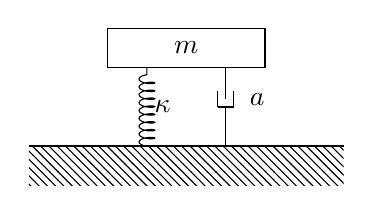
\begin{tikzpicture}
	\draw[decoration={aspect=0.3, segment length=1mm, amplitude=1mm, coil},decorate]
	(1.5, 0) -- (1.5,1);
	
	\draw (1.7, 0.5) node {$\kappa$};
	\draw (2.9, 0.6) node {$a$};
	\draw (2,1.25) node {$m$};
	
	\draw (2.5, 0) -- (2.5, 0.5);
	\draw (2.4, 0.5) -- (2.6, 0.5);
	\draw (2.4, 0.5) -- (2.4, 0.7);
	\draw (2.6, 0.5) -- (2.6, 0.7);
	\draw (2.5, 0.6) -- (2.5, 1);
	
	\draw (1, 1) rectangle (3,1.5);
	
	\fill[pattern=north west lines] (0,-0.5) rectangle (4,0);
	\draw[thick] (0,0) -- (4,0);
	\end{tikzpicture}
	\hspace{20pt}
	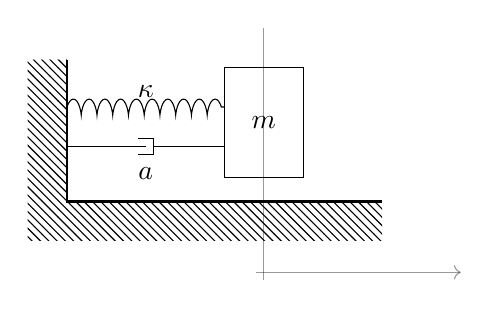
\begin{tikzpicture}
	\draw[decoration={aspect=0.3, segment length=2mm, amplitude=1mm, coil},decorate]
	(0,1.5) -- (2,1.5) node[midway,above] {$\kappa$};
	
	\draw[,opacity=.4] (2.5,-0.7) -- (2.5,2.5);
	\draw[->,opacity=.4] (2.4,-0.6) -- (5,-0.6);
	
	\draw (1, 0.65) node {$a$};
	\draw (2.5,1.3) node {$m$};
	
	\draw (0, 1) -- (1, 1);
	\draw (1.1, 1.1) -- (1.1, 0.9);
	\draw (1.1, 1.1) -- (0.9, 1.1);
	\draw (1.1, 0.9) -- (0.9, 0.9);
	\draw (1.1, 1) -- (2, 1);
	
	\draw (2, 2) rectangle (3,0.6);
	
	\fill[pattern=north west lines] (0,2.1) rectangle (-0.5,0.3) rectangle (4, -0.2);
	\draw[thick] (0,2.1) -- (0,0.3) -- (4,0.3);
	\end{tikzpicture}
    \end{center}
	
	\paragraph{(α)}
	\begin{align*}
	m\ddot{x} &= -\kappa x - a \dot{x} +F(t)
	\intertext{ή}
	\ddot{x}+\frac{a}{m}\dot{x}+\frac{\kappa}{m} &= \frac{F(t)}{m}
	\intertext{ΑΣ}
	\dot{x}(0) &= 150\ \mathrm{ ^{cm}/_s}\\
	x(0) &= 0\\
	\ddot{x}+5x&=0
	\intertext{ΓΡ/ΟΜ/ΔΕ/2τ/ΣΣ}
	\lambda^2+5 = 0 \implies \lambda_{1,2} = \pm i\sqrt{5}\\
	\Aboxed{
		\text{ΓΛ} \quad x(t)&=c_1\cos\sqrt{5}t+c_2\sin\sqrt{5}t
		}\\
		x'(t)&=-c_1\sqrt{5}\sin\sqrt{5}t+c_2\sqrt{5}\cos\sqrt{5}t\\
		x(0)&=0 \implies 0 =\cancelto{1}{c_1\cos\sqrt{5}}(0)+c_2\cancelto{0}{\sin\sqrt{5}(0)} \implies 0 =c_1\\
		\dot{x}(0) &= 1.5 \implies 1.5 = -c_1\sqrt{5}\sin\sqrt{5}(0)+c_2\sqrt{5}\cos\sqrt{5}(0)\implies c_2=\frac{1.5}{\sqrt{5}}
	\end{align*}
	
	\paragraph{(β)}
	\begin{gather*}
	\omega = \sqrt{5}\ \mathrm{rad/s}\\
	f=\frac{\omega}{-2\pi}=\frac{\sqrt{5}}{2\pi}\; \mathrm{Hz}\\
	T=\frac{1}{s}
	\end{gather*}
\end{exercise*}

\subsection{ΓΛ ΜΟ/ΔΕ}
\[
x=\underbrace{x_n}_{\text{ΓΛ ΟΜ}}+\overbrace{x_p}^{???}
\]

\[
\mathbf{L}(x) = \phi(t)
\]

\subsection*{Μέθοδος απροσδιόριστων τελεστών}
\(
\phi(t)
\) και όλες οι παράγωγοί της \(
\left\lbrace x_1,x_2,\dots,x_n \right\rbrace
\)

\paragraph{Αρχικοποίηση}

\[
x_p(t) = \underbrace{A_1x_1(t)+A_2x_2(t) + \dots + A_nx_n(t)}_{\text{αυθαίρετοι}}
\]

\subparagraph{Περίπτωση 1}
\begin{align*}
\phi(t)&=p_n(t)\\
\tilde x_p &= A_nt^n+A_{n-1}t^{n-1}+\dots+A_1t+A_0\quad A_j (j=0,\dots,n)
\end{align*}

\subparagraph{Περίπτωση 2}
\begin{align*}
\phi(t)&=\kappa e^{at}\\
\tilde x_p &= Ae^{at}
\end{align*}

\subparagraph{Περίπτωση 3}
\begin{align*}
\phi(t) &= \kappa_1\sin\beta t + \kappa_2\cos\beta t\\
\tilde x_p &= A\sin\beta t + B\cos\beta t
\end{align*}

\subparagraph{Γενίκευση}
\(
\begin{matrix}
	\phi(t) \text {συνδυασμός περιπτώσεων.}               \\
	\rightarrow \tilde x_p \text{ αντίστοιχος συνδυασμός}
\end{matrix}
\)

\paragraph{Τροποποίηση}
Όταν η \(\widetilde{x}\) έχει κοινό όρο με τη \(x_h\), τότε πολλαπλασιάζουμε με \(t^m\) την \(\widetilde{x_p}\) ώστε να μην υπάρχει κοινός όρος.

\begin{exercise*}{5.24}
	\[y''-y'-2y=4x^2\]
	\tcblower
	βλ. 5.1
	
	\[
	y_h = c_1e^{-x}+c_2e^{2x}
	\]
	
	\begin{gather*}
	\phi(x)=4x^2\\
	\boxed{y_p  = A_2x^2+A_1x+A_0}\\
	y'_p = 2A_2x+1_1\\
	y''_p = 2A_2
		\end{gather*}
		
	Αντικαθιστώντας στη διαφορική μας εξίσωση έχουμε:
	\begin{align*}
	2A_2-(2A_2x+A_1)-2(A_2x^2+A_1x+A_0)&=4x^2 \implies \\
	(-2A_2)x^2+(-2A_2-2A_1)x+(2A_2-A_1-2A_0)&=4x^2+(0)x+0 \implies \\
	\begin{cases}
	-2A_2 &= 4\\
	-2A_2-2A_1 &= 0 \\
	2A_2-A_1-2A_0 &=0
	\end{cases}
	&\implies
	\begin{cases}
	A_2 &= -2 \\
	A_1 &= 2 \\
	A_0 &= -3
	\end{cases} \implies \\
	\Aboxed{y_p &= -2x^2+2x-3} \\
	\text{ΓΛ ΜΟ} 
	\quad
	y = y_h+y_p &= c_1e^{-x}+c_2e^{2x}-2x^2+2x-3
	\end{align*}
\end{exercise*}

\begin{exercise*}{5.25}
	\[
	y''-y'-2y = e^{3x}
	\]
	\tcblower
	5.1 ΟΜ
	
	\(y_h = c_1e^{-x}+c_2e^{2x}\)
	
	\(\phi(x)=e^{3x}, \quad y_p(x) = Ae^{3x}
	\)
	
	\(
	y'_p=3Ae^{3x}, \quad y''_p = 9Ae^{3x}
	\)
	
	\(
	9Ae^{3x}-3Ae^{3x}-2Ae^{3x}=e^{3x} \implies 4Ae^{3x}=e^{3x} \implies 4A=1 \implies \boxed{A = \frac{1}{4}}
	\)
	
	ΕΛ ΜΟ \(y_p = \frac{1}{4} e^{3x}\)
	
	ΓΛ ΜΟ \(y(x) = c_1e^{-x}+c_2e^{2x}+\frac{1}{4}e^{3x} \)
\end{exercise*}

\begin{exercise*}{5.25}
	\[
	y'' -y' -2y = \sin 2x
	\]
	\tcblower
	5.1 OM \(y_h = c_1e^{-x} + c_2e^{2x}\)
	
	\(\phi(x) = \sin 2x \)
	
	\(
	y_p = A\sin 2x + B \cos 2x
	\)
	
	\(y'_p=2A\cos 2x-2B\sin2x \)
	
	\(y''_p=-4A\sin2x-4B\cos2x\)
	
	
	\begin{align*}
	(-4A\sin2x-4B\cos2x) - (2A\cos2x-2B\sin2x)-2(A\sin2x+B\cos2x) &= \sin2x \implies \\
	(-6A+2B)\sin2x+(-6B-2A)\cos2x &= (1)\sin2x+(0)\cos2x \implies \\
	\begin{cases}
	-6A-2B &=1 \\
	-2A-6B &= 0
	\end{cases}
	\implies \begin{cases}
	A &= -\frac{3}{20} \\
	B &= \frac{1}{20} 
	\end{cases} \implies \text{ΕΛ ΜΟ } \Aboxed{ y_p &= -\frac{3}{20}\sin2x+\frac{1}{20}\cos 2x}
	\end{align*}
	
	\[
		\text{ΓΛ ΜΟ } \boxed{
			y = c_1e^{-x} + c_2e^{2} - \frac{3}{20}\sin 2x + \frac{1}{20}\cos 2x
		}
	\]
\end{exercise*}

\begin{exercise*}{5.30}
	\[
	y'''-6y''+11-6y = 2xe^{-x}
	\]
	\tcblower
	5.16 ΟΜ \(y_h = c_1e^x +c_2e^{2x}+c_3e^{3x} \)
	
	\(
	\phi(x) = 2xe^{-x} \quad \phi(x)=e^{ax}p_n(x), \ a=-1,\ p_n(x)=2x
	\)
	
	\(
	y_p = e^{-x}(A_1x+A_0) \implies \boxed{y_p  = A_1xe^{-x}+A_0e^{-x}}
	\)
	
	\(
	y'_p = -A_1xe^{-x} + A_1e^{-x}-A_0e^{-x}
	\)
	
	\(
	y''_p= A_1xe^{-x} -2A_1e^{-x} + A_0e^{-x}
	\)
	
	\(
	y'''_p = -A_1xe^{x} + 3A_1e^{-x} - A_0e^{-x}
	\)
	
	\begin{align*}
	-24A_1xe^{-x} + (26A_1-24A_0)e^{-x} &= 2xe^{-x} + (0)e^{-x} \implies \\
	\begin{cases}
	-24A_1 &= 2 \\
	26A_1-24A_0 &=0
	\end{cases}
	\implies \begin{cases}
	A_1 &= -\frac{1}{12} \\
	A_0 &= -\frac{13}{144}
	\end{cases}
	\text{ΕΛ ΜΟ } y_p &= -\frac{1}{12}xe^-x-\frac{13}{144}e^{-x}\\
	\text{ΓΛ ΜΟ } \Aboxed{ y &= c_1e^x+c_2e^{2x}+c_3e^{3x}-\frac{1}{12}xe^{-x}-\frac{13}{144}e^{-x} }
	\end{align*}
\end{exercise*}

\begin{exercise*}{5.31}
	\[
	y''=9x^2+2x-1
	\]
	
	ΟΜ ΔΕ \(
	y'' = 0, \boxed{y_n=c_1x+c_0}
	\)
	
	\(
	\phi(x) = 9x^2+2x-1 \quad \underbrace{y_p}_{\mathclap{\cdot\; x^m}} = A_2x^2+A_1x+A_0
	\)
	
	\paragraph{Τροποποίηση}
	\(\boxed{
	y_p = A_2x^4+A_1x^3+A_0x^2
} \)

    \(y'_p = \dots,\quad y''_p = \dots\)
    
    \begin{align*}
    12A_2x^2 + 6 A_1x+2A_0 = 9x^2+2x -1 \xRightarrow{\dots} \begin{cases}
    A_2 &= \frac{3}{4}\\
    A_1 &= \frac{1}{3} \\
    A_0 &= -\frac{1}{2} 
    \end{cases} \implies
    \frac{3}{4}x^4+\frac{1}{3}x^3-\frac{1}{2}x^2
    \end{align*}
    
    \[
    \text{ΓΛ ΜΟ }
    y=c_1x+c_0+\frac{3}{4}x^4+\frac{1}{3}x^3-\frac{1}{2}x^2
    \]
\end{exercise*}

\begin{exercise*}{5.36}
	\(RLC\) κύκλωμα σε σειρά, \(R = 180\; \Omega,\ C = \frac{1}{280}\; \mathrm F,\ L=20\; \mathrm H\)
	
	Εφαρμόζεται τάση \(v(t)=10\sin t\), καμία αρχική φόρτιση και αρχικό ρεύμα \(1\; \mathrm A\) για \(t = 0\), οπότε εφαρμόζεται η τάση.
	
	Να βρεθεί το φορτίο στον πυκνωτή.
	\tcblower
	
	\begin{center}
		\begin{circuitikz} \draw
			(0,0) to[vsourcesin=$v(t)$] (0,2)
			to[R=$R$] (2,2) 
			to[L=$L$] (4,2)
			to[C=$C$] (6,2) -- (6,0) -- (0,0);
		\end{circuitikz}
	\end{center}
	
	\begin{gather*}
	Ri + \frac{1}{C}q + L\od{i}{t} -v = 0\\
	i = \od{q}{t} = q \implies \od{i}{t} = \od[2]{q}{t} = \ddot{q}
	\implies R \dot q + \frac{1}{C}q + L \ddot q = v \\
	\implies \boxed{\ddot q + \frac{R}{L} \dot q + \frac{1}{LC} q = \frac{1}{L}v} \quad \text{ΜΟ/ΓΡ/ΔΕ/2-τ/ΣΣ} \\
	q(0)=0,\ i(0)=1\implies \dot q (0) = 1\\
	\ddot q + \frac{180}{20}\dot q + \frac{1}{20\left( ^1/_{180}\right)}q = \frac{10}{20}\sin t \implies \\
	\boxed{
		\ddot q + 9\dot q + 14q = \frac{1}{2}\sin t
		} \quad \text{ΔΕ}\\
		\text{ΓΛ ΟΜ} \quad \ddot q + 9\dot q + 14q = 0 \\
		\text{ΧΕ} \quad \lambda^2 +9\lambda +14=0\\
		\lambda_1=-2,\lambda_2=-7\\
		\text{ΓΛ ΟΜ} \quad \boxed{q_h =c_1e^{-2t}+c_2e^{-7t}} \\
		\text{ΓΛ ΜΟ} \quad q = q_h+q+p\\
		\phi(t) = \frac{1}{2} \sin t\\
		q_p = A\sin t + B\cos t\\
		\dot q_p = A\cos t - B\sin t\\
		\ddot q_p = -A\sin t - B\cos t\\
		-A\sin t - B\cos t + 9 A\cos t - 9B\sin t + 14A\sin t+ 14B\cos t = \frac{1}{2}\sin t \\
		\implies (-A-9B+14A)\sin t + (-B+9A+14B)\cos t = \left(\frac{1}{2}\right)\sin t + \big(0\big)\cos t \\
		\begin{cases}
		13A-9B&=\frac{1}{2}\\
		9A+13B&=0
		\end{cases} \implies \begin{cases}
		A &= \frac{13}{500} \\
		B &= -\frac{9}{500}
		\end{cases}
		\\
		\text{ΕΛ ΜΟ} \quad q_p = \frac{13}{500}\sin t -\frac{9}{500}\cos t\\
		\text{ΓΛ ΜΟ} \quad q = c_1e^{-2t}+c_2e^{-7t}+\frac{13}{500}\sin t - \frac{9}{500}\cos t\\
		\cdots \implies \begin{cases}
		c_1 &= \frac{110}{500} \\
		c_2 &= -\frac{101}{500}
		\end{cases} \xrightarrow{\text{ΕΛΜΟ}} q = \frac{1}{500} (110e^{-2t}-101e^{-7t}+13\sin t-9\cos t)
	\end{gather*}
\end{exercise*}

\subsection{ΓΡ/ΔΕ/ΜΣ: Μέθοδος μεταβολής των παραμέτρων}
\begin{align*}
\begin{matrix}
\text{ΜΟ}\\\text{ΔΕ}\end{matrix}\quad P_0(x)y'' + P_1(x)y'+P_2(x)y &= F(X) \\
\begin{matrix}
\text{ΟΜ}\\\text{ΔΕ}\end{matrix}\quad P_0(x)y'' + P_1(x)y'+P_2(x)y &=0 \\
\text{Σύνολο λύσεων ΟΜ/ΔΕ } \left\lbrace y_1,y_2 \right\rbrace &
\end{align*}
\begin{align*}
\text{ΓΛ ΜΟ}\quad y = & y_p + c_1y_1+c_2y_2=y_p+y_h\\
& y_p \text{ ΕΛ ΜΟ ΔΕ}
\end{align*}

\(P_0,P_1,P_2,F\) συνεχείς \((a,b)\)

\(P_0 \) χωρίς μηδενικά

\paragraph{\textlatin{a})}
\(
y_p = u_1y_1+u_2y_2
\)

\paragraph{\textlatin{b})}
\(
\begin{cases}
u'_1y_1+u'_2y_2 &=0\\
u'_1y'_1+u'_2y'_2 &= \frac{F}{P_0}
\end{cases}
\)

\paragraph{\textlatin{c)}}
\(
u'_1,u'_2
\)

\paragraph{\textlatin{d)}}
υπολογίζουμε \(u_1,u_2\), με ολοκλήρωση (ολ. σταθ \(\rightarrow 0\))

\paragraph{\textlatin{e)}}
αντικατάσταση \(u_1,u_2\) στην \(y_p\)

\begin{exercise*}{6.1}
	\[
	x^2y'' -2xy' -2y = x^{\frac{9}{2}}
	\]

	\(
	y_h = c_1x+c_2x^2 = c_1y_1 + c_2y_2 \text{ ΓΛ ΟΜ}
	\)
	
		\tcblower
	ΕΛ
	\paragraph{\textlatin{a})}
	\begin{align*}
	y_p &= u_1y_1 + u_2y_2 \\
	    &= u_1x   + u_2x^2
	\end{align*}
	
	\paragraph{\textlatin{b})}\[
	\begin{cases}
	u_1'x+u_2'x^2 &=0 \\
	u_1' + 2u_2'x &= \frac{x^{\left( ^9/_2\right)}}{x^2}	
	\end{cases} \impliedby \begin{cases}
	u_1'y_1+u_2'y_2 &= 0\\
	u_1'y_1'+u_2'y_2' &= \frac{F}{P_1}
	\end{cases}
	\]
	
	\paragraph{\textlatin{c})}
	\begin{align*}
	u_1' &= -u_2' x\\
	u_2'x &= x ^ {^5/_2} \implies u_2' = x^{^3/_2}, u_1' = -x^{^5/_2}
	\end{align*}
	
	\paragraph{\textlatin{d}) ολοκλήρωση}
	\[
	u_1=-\frac{2}{7}x^{^7/_2},\ u_2=\frac{2}{5}x^{^5/_2}
	\]
	
	\paragraph{\textlatin{e})}
	\[
	y_p = -\frac{2}{7}x^{^7/_2}x + \frac{2}{5}x^{^5/_2}x^2 = \frac{4}{35}x^{^9/_2}
	\]
	
	\[
	\boxed{
		y=y_h+y_p=c_1+c_2x^2+\frac{4}{35}x^{^9/_2}
		} \quad \text{ΓΛ ΜΟ}
	\]
\end{exercise*}
%TODO Copy notes

\begin{exercise*}{12.4}
	\(y''-3y'+4y=0, \quad y(0)=1,\ y'(0)=5\)
	\tcblower
	\[
	\mathscr L \left\lbrace y'' \right\rbrace - 3\mathscr L\left\lbrace y' \right\rbrace
	+4\mathscr L\left\lbrace y \right\rbrace = \mathscr L\left\lbrace 0 \right\rbrace
	\]
	
	\( \left[s^2Y(s)-y-5\right] -3\left[sY(s)-1 \right] + 4Y(s) = 0\) \\
	\( \implies Y(s) = \frac{s+2}{s^2-3s+4} \)
	
    Παρονομαστής \( s^2-3s+4 = (s^2-3s)+4 = \left[ s^2-3s+\left(
    \frac{-3}{2}
    \right)^2 \right] + 
    \left[ 4-\left(
    \frac{-3}{2}
    \right)^2 \right] = \left(
    s-\frac{3}{2}
    \right)^2 + \left(\frac{\sqrt{7}}{2}\right)^2
    \)
    
    Αριθμητής: \( s+2 = \left(s-\frac{3}{2}\right) + \frac{7}{2} 
    = \left(s-\frac{3}{2}\right)+ \sqrt{7}\frac{\sqrt{7}}{2}
    \)
    
    Άρα \begin{align*} 
    Y(s) &= \frac{(s-^3/_2)+\sqrt{7}\frac{\sqrt{7}}{2}}{(s-^3/_2)^2+\left(\frac{\sqrt{7}}{2}\right)^2}
    \\ &=
    \frac{s-^3/_2}{(s- ^3/_2)^2+\left(\frac{\sqrt{7}}{2}\right)}+\sqrt{7}\frac{\frac{\sqrt{7}}{2}}{(s-^3/_2)^2+\left(\frac{\sqrt{7}}{2}\right)} \\
    \implies y(x) &= \mathscr L^{-1} \left\lbrace Y(s) \right\rbrace = \\
    &= \mathscr L^{-1}\left\lbrace 
    \frac{s-^3/_2}{(s- ^3/_2)^2+\left(\frac{\sqrt{7}}{2}\right)}
    \right\rbrace + \sqrt{7} \mathscr L^{-1} \left\lbrace 
    \frac{\frac{\sqrt{7}}{2}}{(s-^3/_2)^2+\left(\frac{\sqrt{7}}{2}\right)}
     \right\rbrace \\
     \implies y(x) &= e^{\frac{3}{2}x}\cos(\frac{\sqrt{7}}{2}x)+\sqrt{7}e^{\frac{3}{2}x}\sin(\frac{\sqrt{7}}{2}x)
     \end{align*}
\end{exercise*}

\begin{exercise*}{12.5}
	\( y''-4y=2e^{3t},\quad y(0)=1,\ y'(0)=-1 \)
	\tcblower
	\( \mathscr L \left\lbrace y' \right\rbrace -4\mathscr L \left\lbrace y \right\rbrace = 2 \mathscr L\left\lbrace e^{3t} \right\rbrace \implies \)
	
	\( \implies \left[
	s^2Y(s)-s+1
	\right] + \left[-4Y(s)\right] = \frac{2}{s-3} \implies \)
	
	\( (s^2-4)Y(s) = \frac{2}{s-3}+s-1=\frac{2+(s-1)(s-3)}{s-3} \xRightarrow{s^2-4=(s-2)(s+2)} \implies Y(s) = \frac{2+(s-1)(s-3)}{(s-2)(s+2)(s-3)} \)
	
	\begin{attnbox}{}
		\[
		\frac{1}{(s-a)^m} \rightarrow \frac{A_1}{(s-a)}+\frac{A_2}{(s-a)^2}+\dots + \frac{A_m}{(s-a)^m}
		\]
		
		\[
		\frac{1}{(s^2+bs+c)^p} \rightarrow 
		\frac{B_1s+C_1}{s^2+bs+c} + \frac{B_2s+C_2}{(s^2+bs+c)^2} + \dots + \frac{B_ps+C_p}{(s^2+bs+c)^p}
		\]
	\end{attnbox}
	
	\( \implies Y(s) = \frac{A}{s-2}+\frac{B}{s+2} + \frac{c}{s-3} \implies  \)
	
	\( \implies \frac{s^2-4s+5}{(s-2)(s+2)(s-3)} = \frac{A(s+2)(s+3)+B(s-2)(s-3)+C(s-2)(s+2)}{(s-2)(s+2)(s-3)} \implies \)
	
	\( s^2-4s+5 = As^2-3As+2As-6A +Bs^2-3Bs-2Bs+6B+Cs^2+2Cs-2Cs-4C \)
	
	\( s^2-4s+5 = (A+B+C)s^2 - (-A-5B)s + (-6A+6B-4C) \implies \begin{cases}
	A+B+C &= 1 \\
	-A-5B &= 4 \\
	-6A +6B -4C &= 5
	\end{cases} \xRightarrow{\dots} \begin{cases}
	A &= -\frac{1}{4} \\
	B &= \frac{17}{30} \\
	C &= \frac{3}{5}
	\end{cases} \)
	
	\( Y(s) = -\frac{1}{4}\frac{1}{s-2} + \frac{17}{20} \frac{1}{s+2} + \frac{2}{5}\frac{1}{s-3} \) 
	
	\[ \implies \boxed{ y(x) = -\frac{1}{4}e^{2x}+\frac{17}{20}e^{-2x}+\frac{2}{5}e^{3x}} \]
\end{exercise*}

\begin{exercise*}{12.6}
	\[
	y''+3y'+2y=6e^t,\quad y(0) = 1,\ y'(0) = -1
	\]
	\tcblower
	\( \left[s^2Y(s)-s+1\right] +3\left[sY(s)-1\right]+2Y(s) = 6\frac{1}{s-1}
	\implies \) \\
	\( (s^2+3s+2)Y(s) = \frac{6}{s-1}+(s-1)+3 = \frac{6+(s-1)(s+2)}{s-1} \) \\
	Εφόσον \( s^2+3s+2=(s+1)(s+2) \)
	
	\( \implies Y(s) = \frac{6+(s-1)(s+2)}{(s-1)(s+2)(s+1)} 
	= \frac{1}{s-1}+\frac{2}{s+2}-\frac{2}{s+1}
	\implies \boxed{ y(t) = e^t+2e^{-2t}-e^{-t} }
	\)
\end{exercise*}

\begin{attnbox}{Προσοχή}
	Σημαντικός ο ύπνος για τις εξετάσεις
\end{attnbox}

\begin{exercise*}{}
	\[y''-2y'-3y=10\cos t\]
	
	\tcblower
	
	\begin{alignat*}{3}
		& \left[s^2Y(s)-2s-7\right]-2\left[sY(s)-2\right]-3Y(s)=\frac{10s}{s^2 + 1} && \implies \\
		\implies & (\underbrace{s^2-2s-3}_{\mathclap{(s-3)(s-1)}})Y(s) = \frac{10s}{s^2+1} + (7+2s)-4 = \frac{10s}{s^2+1}+(2s+3) && \implies \\
		\implies & Y(s) = \frac{10s}{(s-3)(s+1)(s^2+1)} + \frac{2s+3}{(s-3)(s+1)} &&
	\end{alignat*}

    \[
    \frac{2s+3}{(s-3)(s+1)} = \frac{9}{4}\frac{1}{s-3}-\frac{1}{4}\frac{1}{s+1} \xleftrightarrow{\mathscr L^{-1}} \frac{9}{4}e^{3t}-\frac{1}{4}e^{-t}
    \]
    
    \[
    \frac{10s}{(s-3)(s+1)(s^2+1)} = \frac{A}{s-3} + \frac{B}{s+1} + \frac{Cs+D}{s^2+1}
    \]
    όπου \( \left(A(s+1)-B(s-3)\right) (s^2+1)+ (Cs+D)(s-3)(s+1)=10s \)
    
    Θέτω \( 
    \begin{array}{l}
    s = 3 \rightarrow \left(A(3+1) + 0\right)(3^2+1)+(\quad)(0)(\quad)=10\cdot 3\implies 40A=30 \\
    s = 1 \rightarrow -8B=-10 \\
    s=0 \rightarrow A-3B-3D = 0 \\
    \text{εξ. συντ } \rightarrow A+B+C = 0
    \end{array} \implies \begin{cases}
    A &= \frac{3}{4} \\
    B &= \frac{5}{4} \\
    C &= -2 \\ 
    D &= -1
    \end{cases}
     \)
     
     \begin{align*}
     \frac{10s}{(s-3)(s+1)(s^2+1)} &= \frac{3}{4}\frac{1}{s-3} + \frac{5}{4}\frac{1}{s+1}-\frac{2s+1}{s^2+1} \\
     &\xleftrightarrow{\mathscr L^{-1}}\frac{3}{4}e^{3t}+\frac{5}{4}e^{-t}-2\cos t - \sin t \\
     \implies & \boxed{
     	y(t) = -\sin t -2\cos t + 3e^{3t}+e^{-t}
     	}
     \end{align*}
     
     
\end{exercise*}

\begin{attnbox}{}
	\[
	e^{ax}\cos bx \leftrightarrow \frac{s-a}{(s-a)^2+b^2}
	\]
	\tcblower
	\[
	e^{ax}\sin bx \leftrightarrow \frac{b}{(s-a)^2+b^2}
	\]
	
	\end{attnbox}


\begin{exercise*}{12.8}
	\[
	y''+4y = 8\sin 2t + 9\cos t,\quad y(0)=1,\ y'(0) = 0
	\]
	\tcblower
	\begin{alignat*}{3}
	& \left[s^2Y(s)-1s-0\right] + 4Y(s) = \frac{16}{s^2+4}+\frac{9s}{s^2+1} && \implies \\
	\implies & Y(s) = \frac{16}{(s^2+4)^2}+\frac{9s}{(s^2+1)(s^2+4)} + \frac{s}{s^2+4} && 
	\end{alignat*}
	
	Γνωρίζουμε ότι \( t\cos(at) \leftrightarrow \frac{s^2-a^2}{(s^2+a^2)^2} \implies
	t\cos 2t \leftrightarrow \frac{s^2-4}{(s^2+4)^2} = \frac{s^2+4}{(s^2+4)^2} - \frac{8}{(s^2+4)^2}
	= \frac{1}{s^2+4}-\frac{8}{(s^2+4)^2}
	 \).
	 
	 Άρα \( \frac{8}{(s^2+4)^2} = \frac{1}{s^2+4} - \mathscr L \left\lbrace t\cos 2t \right\rbrace 
	 \implies \frac{16}{(s^2+4)^2} \xleftrightarrow{\mathscr L^{-1}}\sin 2t-2t\cos 2t
	 \)
	 
	 Αντικαθιστώντας \( x=s^2 \) στον \( \frac{9}{(x+4)(x+1)} = \frac{3}{x+1}-\frac{3}{x+4} \) και πολλαπλασιάζοντας με \( s \), μάς δίνει \( \frac{9s}{(s^2+4)(s^2+1)} = \frac{3s}{s^2+1} -\frac{3s}{s^2+4} \xleftrightarrow{\mathscr L^{-1}}3\cos t-3\cos 2t \).
	 
	 \( \frac{s}{s^2+4} \xleftrightarrow{\mathscr L^{-1}} \cos 2t \)
	 
	 \[
	 \boxed{
	 	y(t) = -(2t+2)\cos 2t + \sin 2t +3\cos tp
	 	}
	 \]
\end{exercise*}


\begin{exercise*}{12.9}
	\[
	y''-2y'+2y=2t,\quad y(0) = 2, \ y'(0) = -7
	\]
	\tcblower
	\begin{align*}
	& \left[s^2Y(s)-2s+7\right]+2\left[sY(s)-2\right]+2Y(s) = \frac{2}{s^2} \implies \\
	\implies & (s^2+2s+2)Y(s) = \frac{2}{s^2}+(2s-7)+4=\frac{2}{s^2}+2s -3
	\end{align*}
	
	Εφ' όσον \( s^2+2s+2 =(s+1)^2+1 \implies Y(s) = \frac{2}{s^2\left((s+1)^2+1\right)}
	+\frac{2s-3}{(s+1)^2+1}
	\)
	
	\[
	\frac{2s-3}{(s+1)^2+1} = \frac{2(s+1)-5}{(s+1)^2+1}=2\frac{s+1}{(s+1)^2+1}-5\frac{1}{(s+1)^2+1}
	\xleftrightarrow{\mathscr L^{-1}}2e^{-t}\cos t-5e^{-t}\sin t
	\]
	
	\[
	\frac{2}{s^2\left((s+1)^2+1\right)} = \frac{A}{s} + \frac{B}{s^2} + \frac{Cs+D}{(s+1)^2+1}
	\]
	όπου \( (As+B)\left((s+1)^2+1\right) + s^2\left(C(s+1)+D\right) =2 \) \\
	\( \implies (A+C)s^3+(2A+B+C+D)s^2 + 2(A+B)s+2B = 2 \) \\
	\( \implies \begin{cases}
	2B&= 2 \quad s = 0\\
	-A+B+D &= 2 \quad s = -1 \\
	A+C &= 0 \quad \text{εξ. συντ. } s^3 \\
	2A+B+C+D &=0 \quad \text{εξ. συντ. } s^2
	\end{cases} \)
	
	Λύνοντας \( 
	\begin{cases}
	A &= -1 \\ B &= 1 \\ C &= 1 \\ D &= 0
	\end{cases}
	 \). Συνεπώς \( \frac{2}{s^2\left((s+1)^2+1\right)} = \frac{1}{s}+\frac{1}{s^2}+ \frac{s+}{(s+1)^2+1} 
	 \leftrightarrow -1+t+e^{-t}\cos t
	 \)
\end{exercise*}


\begin{exercise*}{12.10}
	\[
	y''-4y'+5y = e^{-t\left(\cos t +3\sin t \right)}
	\]
	\( y(0) = 0,\ y'(0) = 4 \)
	\tcblower
	\( 
	\left[s^2Y(s)-4s\right]+4\left[sY(s)-0\right] = \frac{s+1}{(s+1)^2+1}+\frac{3}{(s+1)^2+1} \implies
	 \)
	 
	 \begin{tcolorbox}{}
	 \( \mathscr L\left\lbrace \od[n]{y}{x} \right\rbrace 
	 = s^nY(s)-s^{n-1}y(0)-s^{n-2}y'(0)-\dots - sy^{(n-2)}-y^{(n-1)}(0)
	 \)
	 \end{tcolorbox}
	 
	 \( 
	 \implies \underbrace{(s^2+4s+5)}_{\mathclap{=(s+2)^2+1 }}Y(s)=\frac{s+4}{(s+1)^2+1}+4 \implies
	  \)
	  
	\( 
	Y(s) = \frac{s+4}{\left((s+1)^2+1\right)\left((s+2)^2+1\right)}
	+\underbrace{\frac{4}{(s+2)^2+1}}_{\mathclap{4e^{-2t}\sin t}}
	\implies 
	 \)
	 
	 \(  \frac{s+4}{\left( (s+1)^2+1 \right)\left( (s+1)^2+1 \right)}
	 = \frac{A(s+1)+B}{(s+1)^2+1}+\frac{C(s+2)+D}{(s+2)^2+1} \implies
	  \)
	  
\( 
\implies
	\left(
	A(s+1)+B
	\right)\left((s+2)^2+1\right)+\left(C(s+2)+D\right)\left((s+1)^2+1\right) = 4+s
\implies
	\begin{cases}
	5A+5B+4C+2D &= 4, \quad \text{για } s=0 \\
	2B+C+D &= 3, \quad \text{για } s=-1\\
	-A+B+2D&=2, \quad \text{για } s=-2\\
	A+C&=0 \quad \text{εξ. συντ του } s^3
	\end{cases} \implies \begin{cases}
	A &= -1\\B&=1\\C&=1\\D&=0
	\end{cases}
\) 

Άρα \(\cdots =  \frac{-(s+1)+1}{(s+1)^2+1} + \frac{s+2}{(s+2)^2+1} =e^{-t}(-\cos t + \sin t) + e^{-2t}\cos t  \)

Άρα \( \boxed{y(t) = e^{-t}(-\cos t + \sin t)+e^{-2t}(\cos t + 4\sin t)} \)
	\end{exercise*}
	
	\begin{exercise*}{12.11}
		\[
		4y''+4y'+y=3\sin t + \cos t
		\]
		\( y(0) = 2,\ y'(0)=-1 \)
	\tcblower
	\begin{gather*}
	4\left[s^2Y(s)-2s+1\right] + 4\left[sY(s)-2\right]+Y(s)=\frac{3}{s^2+1}+\frac{s}{s^2+1} \\
	\implies \underbrace{(4s^2+4s+1)}_{\mathclap{4\left(s+\frac{1}{2}\right)^2}}Y(s) = \frac{3+s}{s^2_1}+4(-1+2s)+8=\frac{3+s}{s^2+1}+8s+4
	\\ \implies
	Y(s) = \frac{3+s}{4\left(s+^1/_2\right)(s^2+1)} + \frac{2}{s+^1/_2}
	\\ \frac{3+s}{4\left(s+^1/_2\right)(s^2+1)} 
	= \frac{A}{s+^1/_2}+ \frac{B}{\left(s+^1/_2\right)^2}+\frac{Cs+D}{s^2+1} \\
	\implies \left(A(s+^1/_2)+B\right)+\left(s^2+1\right)+(Cs+D)\left(s+\frac{1}{2}\right)^2=\frac{3+s}{4} \\ \implies
	\begin{cases}
	\text{για } s = - \frac{1}{2} \rightarrow 10B &= 5 \\
	\text{για } s = 0 \rightarrow 2A +4B + D &= 3 \\
	\text{για } s = 1 \rightarrow 12A+8B+9C+9D &=4 \\
	\text{εξ. αντ. συντ. } s^3 \rightarrow A+C &= 0
	\end{cases} \implies \begin{cases}
	A &= ^3/_5 \\
	B &= ^1/_2 \\
	C &= -^3/_5 \\
	D &= -^1/_5
	\end{cases} \\
	\implies \frac{3+s}{4\left(s+^1/_2\right)^2(s^2+1)} = \frac{3}{5} \frac{1}{s+^1/_2}+\frac{1}{2}\frac{1}{\left(s+^1/_2\right)^2}-\frac{1}{5}\frac{3s+1}{s^2+1} \leftrightarrow \frac{3}{5}e^{-\frac{t}{2}}+\frac{1}{2}te^{-\frac{t}{2}}-\frac{1}{5}\cdot (3\cos t +\sin t)\\
	\frac{2}{1+ ^1/_2} \leftrightarrow 2e^{-\frac{t}{2}} \implies
	\boxed{y(t) = \frac{e^{- ^t/_2}}{10}}\left(5t+26\right)-\frac{1}{5}(3\cos t+\sin t)
	\end{gather*}
	\end{exercise*}

\section{Συστήματα Διαφορικών Εξισώσεων}

\begin{exercise*}{12.12} \[
	\begin{cases}
		u'+u-v &=0 \\
		u'-u+v &= 2	
	\end{cases}
	\]
	\begin{align*}
	u(0) &= 1 \\
	v(0) &= 2
	\end{align*}
	\tcblower
	\begin{align*}
	\mathscr L\left\lbrace u(x) \right\rbrace &= U(s) \\
	\mathscr L\left\lbrace v(x) \right\rbrace &= V(s)
	\end{align*}
	\begin{align*}
&	\begin{cases}
	\left[sU(s)-1\right]+U(s)-V(s) &=0 \\
	\left[sV(s)-2\right]-U(s)+V(s) &= \frac{2}{s}
	\end{cases} \\ \implies& \begin{cases}
	(s+1)U(s) - V(s) &= 1 \\
	-U(s) + (s+1)V(s) &= \frac{2(s+1)}{s}
	\end{cases} \\ \implies &
	\begin{cases}
	U(s) &= \frac{s+1}{s^2} \\ V(s) &= \frac{2s+1}{s^2}
	\end{cases} \\ \implies&
	\begin{cases}
	\mathscr L^{-1} \left\lbrace U(s) \right\rbrace = \mathscr L^{-1} \left\lbrace \frac{s+1}{s^2} \right\rbrace = \mathscr L^{-1} \left\lbrace \frac{1}{s} +\frac{1}{s^2}\right\rbrace \implies u(x) &= 1+x \\
	\mathscr L^{-1}\left\lbrace V(s) \right\rbrace =  \mathscr L ^{-1}\left\lbrace \frac{2s+1}{s^2} \right\rbrace =  \mathscr L ^{-1}\left\lbrace \frac{2}{s} + \frac{1}{s^2} \right\rbrace \implies v(x) &= 2+x
	\end{cases}
	\end{align*}
	\end{exercise*}

\begin{exercise*}{12.13}
	\[
	y'+z=x,\ z'+4y=0,\ y(0)=1,\ z(0)=-1
	\]
	\tcblower
	\begin{align*}
	 &\mathscr L \left\lbrace y(x) \right\rbrace = Y(s),\  \mathscr L \left\lbrace z(x) \right\rbrace = Z(s) \\
	 \implies &
	 \begin{cases}
	 \left[sY(s)-1\right]+Z(s) &= \frac{1}{s^2} \\
	 \left[sZ(s)+1\right]+4Y(s) &=0
	 \end{cases}
	 \\ \implies &
	 \begin{cases}
	 sY(s) + Z(s) &= \frac{s^2+1}{s^2} \\
	 4Y(s) + sZ(s) &= -1
	 \end{cases}
	 \\ \implies &
	 \begin{cases}
	 Y(s) &= \frac{s^2+s+1}{s(s^2-4)} \\
	 Z(s) &= -\frac{s^3+4s^2+4}{s^2(s^2+4)}
	 \end{cases}
	\end{align*}
	
	\begin{align*}
	\frac{s^2+s+1}{s(s^2-4)} = \frac{s^2+s+1}{s(s+2)(s-2)} = \frac{A}{s} + \frac{B}{s+2} + \frac{C}{s-2} \\
	\implies s^2+s+1 = (A+B+C)s^2+2(C-B)s-4A \\
	\implies \begin{cases}
	A+B+C &= 1 \\
	2(C-B) &= 1 \\
	-4A &= 1
	\end{cases} \\
	\implies \begin{cases}
	A &= - \frac{1}{4} \\
	B &= \frac{3}{8} \\
	C &= \frac{7}{8}
	\end{cases} \\
	Y(s) = \frac{- ^1/_4}{s}+\frac{^3/_8}{s+2}+\frac{^7/_8}{s-2} \leftrightarrow \boxed{y(x) = -\frac{1}{4}+\frac{3}{8}e^{2x}+\frac{7}{8}e^{2x}}
	\end{align*}
	
	Από την 1\textsuperscript{η} σχέση,
	\[
	\boxed{z = x+\frac{3}{4}e^{-2x}-\frac{7}{4}e^{2x}}
	\]
\end{exercise*}

\begin{exercise*}{12.14}\[
	\left.
	\begin{cases}
		w'+y &= \sin x \\
		y'-z &= e^x \\
		z'+w+y &= 1
	\end{cases}
	\middle|
	\begin{array}{l}
	w(0)=0\\y(0)=1\\z(0)=1
	\end{array}
	\right.
	\]
	\tcblower
	\begin{align*}
	&\begin{cases}
		\left[sW(s)-0\right]+Y(s) &= \frac{1}{s^2+1} \\
		\left[sY(s)-1\right]-Z(s) &= \frac{1}{s-1} \\
		\left[sZ(s)-1\right]+W(s)+Y(s) &= \frac{1}{s}
	\end{cases}
	\\ &\implies
	\begin{cases}
	sW(s)+Y(s)&= \frac{1}{s^2+1} \\
	sY(s)-Z(s) &= \frac{s}{s+1} \\
	W(s)+Y(s)+sZ(s) &= \frac{s+1}{s}
	\end{cases} \\ &\implies \begin{cases}
	W(s) &= \frac{-1}{s(s-1)} \\
	Y(s) &= \frac{s^2+s}{(s-1)(s^2+1)} \\
	Z(s) &= \frac{s}{s^2+1}
	\end{cases}
	\\ &\implies
	\begin{cases}
	w(x) &= 1-e^x \\
	y(x) &= e^x-\sin x\\
	z(x) &= \cos x
	\end{cases}
	\end{align*}
\end{exercise*}


\begin{exercise*}{12.15}
	\begin{align*}
	y''+z+y &= 0 \\ 
	z'+y' &= 0
	\end{align*}
	\begin{align*}
	y(0) &= 0 \\ y'(0) &= 0 \\ z(0)&=1
	\end{align*}
	\tcblower
	\begin{align*}
	\implies& \begin{cases}
	\left[s^2Y(s)-(0)s-(0)\right] + Z(s) + Y(s) &= 0 \\
	\left[sZ(s)-1\right]+\left[sY(s)-0\right] &= 0
	\end{cases}
	\\ \implies & \begin{cases}
	(s^2+1)Y(s)+Z(s) &= 0\\
	Y(s) + Z(s) &= \frac{1}{s}
	\end{cases}
	\\ \implies & \begin{cases}
	Y(s) &= -\frac{1}{s^3} \\
	Z(s) &= \frac{1}{s} + \frac{1}{s^3}
	\end{cases} \\ \implies & \begin{cases}
	y(x) &= -\frac{1}{2}x^2 \\
	z(x) &= 1 + \frac{1}{2}x^2
	\end{cases}
	\end{align*}
\end{exercise*}

\begin{exercise*}{12.16}
	\[
	\begin{cases}
	z''+y'&=\cos x \\
	y''-z&=\sin x
	\end{cases}
	\]
	\begin{align*}
	z(0) &= -1\\
	z'(0) &= -1 \\
	y(0) &= 1 \\
	y'(0) &= 0
	\end{align*}
	\tcblower
	\begin{align*}
	& \begin{cases}
	\left[s^2Z(s)+s+1\right]+\left[sY(s-1)\right] &= \frac{s}{s^2+1} \\
	\left[s^2Y(s)-s-0\right]-Z(s) &= \frac{1}{s^2+1}
	\end{cases} \\ &\implies 
	\begin{cases}
	s^2Z(s)+sY(s) &= -\frac{s^3}{s^2+1} \\
	-Z(s)+s^2Y(s) &= \frac{s^3+s+1}{s^2-1}
	\end{cases} \\
	& \implies \begin{cases}
	Z(s) &= -\frac{s+1}{s^2+1} \\
	Y(s) &= \frac{s}{s^2+1}
	\end{cases} \\
	& \implies \begin{cases}
	z(x) &= -\cos x-\sin x \\
	y(x) &= \cos x
	\end{cases}
	\end{align*}
\end{exercise*}

\begin{exercise*}{12.17}
	\[
	\begin{cases}
	w''-y+2z &= 3e^{-x} \\
	-2w'+2y'+z &= 0 \\
	2w'-2y+z'+2z'' &= 0 
	\end{cases}
	\]
	\begin{align*}
	w(0)=1 \quad & y(0) = 2 \\
	w'(0)=1 \quad & z(0) = 2 \\
	& z'(0) = -2
	\end{align*}
	\tcblower
	\begin{align*}
	& \begin{cases}
	\left[s^2W(s)-s-1\right]-Y(s)+2Z(s) &= \frac{3}{s+1} \\
	-2\left[sW(s)-1\right]+2\left[sY(s)-2\right]+Z(s) &= 0 \\
	2\left[sW(s)-1\right]-2Y(s) + \left[sZs-2\right]+2\left[s^2Z(s)-2s+2\right] &= 0
	\end{cases} \\ \implies &
	\begin{cases}
	s^2W(s) - Y(s)+2Z(s) &= \frac{s^2+2s+4}{s+1} \\
	-2sW(s)+2sY(s)+Z(s) &= 2 \\
	2sW(s)-2Y(s)+(2s^2+s)Z(s) &= 4s
	\end{cases} \\ \implies &
	\begin{cases}
	W(s) &= \frac{1}{s-1} \leftrightarrow e^x =w(x) \\
	Y(s) &= \frac{2s}{(s-1)(s+1)} = \frac{1}{s-1}+\frac{1}{s+1} \leftrightarrow e^x+e^{-x}=y(x) \\
	Z(s) &= \frac{2}{s+1} \leftrightarrow 2e^{-x}=z(x)
	\end{cases}
	\end{align*}
\end{exercise*}

\section{Επίλυση ΓΡ ΔΕ με γενικευμένες/ασυνεχείς συναρτήσεις ως πηγές}
\paragraph{Βηματική συνάρτηση \( u \)}
\[
u(t)= \begin{cases}
0 \quad t<0 \\
1 \quad t \geq0
\end{cases}
\]

\paragraph{Μετατοπισμένη βηματική συνάρτηση}
\[
u(t-c)=u_c(t)
\]
\[
u_c(t) = \begin{cases}
0 \quad t < c \\
1 \quad t \geq c
\end{cases}
\]

\paragraph{Συνάρτηση τινάγματος ή πάγκου \textlatin{(bench)}}
\begin{align*}
b(t) &= u(t-a)-u(t-b)\\
b(t) &= \begin{cases}
0 \quad t <a \\
1 \quad a \leq t \leq b \\
0 \quad b \leq t
\end{cases}
\end{align*}

\begin{figure}
	\centering
	\begin{subfigure}[b]{0.31\textwidth}
		\begin{tikzpicture}[scale=0.8]
		\begin{axis}[%
		gray
		,xlabel=$t$
		,ylabel=$u(t)$
		,axis lines = center
		,ymax=1.5
		,ytick={0,1}
		,xtick={0}
		]
		\addplot+[const plot, no marks,very thick] coordinates {(-4,0) (0,1) (4,1)} node[above,pos=.57,black] {$u$};
		
		\end{axis}
		\end{tikzpicture}
		\caption{Βηματική συνάρτηση \(u\)}
	\end{subfigure}
	~
	\begin{subfigure}[b]{0.31\textwidth}
		\begin{tikzpicture}[scale=0.8]
		\begin{axis}[%
		gray
		,xlabel=$t$
		,ylabel=$u(t)$
		,axis lines = center
		,ymax=1.5
		,ytick={0,1}
		,xtick={0,1}
		,xticklabels={$0$,$c$}
		]
		\addplot+[const plot, no marks,very thick] coordinates {(-4,0) (1,1) (4,1)} node[below,pos=.57,black] {$u_c$};
		
		\end{axis}
		\end{tikzpicture}
		\caption{Μετατοπισμένη βηματική \(u_c\)}
	\end{subfigure}
	~
	\begin{subfigure}[b]{0.31\textwidth}
		\begin{tikzpicture}[scale=0.8]
		\begin{axis}[%
		gray
		,xlabel=$t$
		,ylabel=$u(t)$
		,axis lines = center
		,ymax=1.5
		,ytick={0,1}
		,xtick={0,-1,1.5}
		,xticklabels={$0$,$a$,$b$}
		,xmin=-2.5
		,xmax=2.5
		]
		\addplot+[const plot, no marks,very thick] coordinates {(-4,0) (-1,1) (1.5,0) (4,0)} node[above,pos=.35,black] {$b$};
		\end{axis}
		\end{tikzpicture}
		\caption{Συνάρτηση πάγκου \(b\)}
	\end{subfigure}
\end{figure}

\begin{align*}
u(t-c) & \leftrightarrow e^{-cs}\frac{1}{s}\\
u(t-c)f(t-c) &\leftrightarrow e^{-cs}F(s) \\
e^{ct}f(t) &\leftrightarrow F(s-c)
\end{align*}

\begin{exercise*}{13.1}
	\[
	y'+2y=u(t-4)
	\]
	\( y(0)=3 \)
	\tcblower
	\( [sY(s)-3]+2Y(s) = e^{-4s}\frac{1}{s} \)
	\( \implies Y(s) = e^{-4s}\frac{1}{s(s+2)}+\frac{3}{s+2} \)
	
	\begin{align*}
	\frac{3}{s+2} &\leftrightarrow 3e^{-2t}\\
	\frac{1}{s(s+2)} = \frac{A}{s} + \frac{B}{s+2} = \frac{A(s+2)+Bs}{s(s+2)} = \frac{A(+b)s+(2A)}{s(s+2)} \\
	\implies \begin{cases}
	A+B&=0\\2A&=1
	\end{cases} \implies \begin{cases}
A &= ^1/_2 \\ B&= - ^1/_2
	\end{cases} \\
	\frac{1}{s(s+2)} = \frac{1}{2} \left[\frac{1}{s}-\frac{1}{s+2}\right]
	\\ \implies e^{-4s}\frac{1}{s(s+2)} = \frac{1}{2} \left(
	e^{-4s}\frac{1}{s}-e^{-4s}\frac{1}{s}-e^{-4s}\frac{1}{s+2}
	\right) &\leftrightarrow \frac{1}{2}\left(u(t-4)-u(t-4)e^{-2(t-4)}\right) 
	\\
	\implies \boxed{
		y(t) = \frac{1}{2}u(t-4)\left(1-e^{-2(t-4)}\right)+3e^{-2t}
	}
\end{align*}
\end{exercise*}

\begin{exercise*}{13.2}
	\( y''+y'+\frac{5}{4}y=b(t) \)
	\( y(0)=0,\ y'(0)=0 \)
	\( b(t) = \begin{cases}
	1 \quad	 0 \leq t \leq \pi \\ 0 \quad t \geq \pi
	\end{cases} \)
	\tcblower
	\begin{centering}
		\begin{tikzpicture}
		\begin{axis}[%
		%    gray
		,xlabel=$t$
		%    ,ylabel=$u(t)$
		,axis lines = center
		,ymax=1.5
		%    ,axis x line = bottom,axis y line = left
		,ytick={0,1}
		,xtick={0,3.14}
		,xticklabels={$0$,$\pi$}
		,xmin=-1
		,xmax=7
		]
		\addplot+[const plot, no marks,very thick,color=magenta] coordinates {(-1,1) (3.14,0) (7,0)} node[midway,anchor=east,black] {$b(t)$};
		\end{axis}
		\end{tikzpicture}
		~
		\begin{tikzpicture}
		\begin{axis}[%
		%    gray
		,xlabel=$t$
		%    ,ylabel=$u(t)$
		,axis lines = center
		,ymax=1.5
		%    ,axis x line = bottom,axis y line = left
		,ytick={0,1}
		,xtick={0,3.14}
		,xticklabels={$0$,$\pi$}
		,xmin=-1
		,xmax=7
		%    ,ymax=1.2 % or enlarge y limits=upper
		%    ,xmin=-1.2
		]
		%\addplot+[const plot, no marks,thick,opacity=1] coordinates {(-1,0) (3.14,1) (7,1)} node[midway,anchor=east,black] {$b(t)$};
		\addplot+[const plot, no marks,very thick,opacity=0.75] coordinates {(-1,0) (0,1) (7,1)} node[pos=0.3,anchor=south,black] {$\mathrm u(t)$};
		\addplot+[const plot, no marks,very thick,color=red,opacity=0.75] coordinates {(-1,0) (3.14,1) (7,1)} node[right,pos=0.3,black] {$\mathrm u(t-\pi)$};
		\addplot+[const plot, no marks,very thick,color=orange,opacity=0] coordinates {(-1,1) (3.14,0) (7,0)} node[midway,anchor=east,black] {$b(t)$};
		%\addplot+[const plot, blue, no marks,very thick] coordinates {(-4,0) (1,1) (4,1)} node[below,pos=.57,black] {$u_c$};
		%\addplot+[const plot, no marks, thick] coordinates {(0,0) (1,0.25) (2,0.4) (3,0.5) (4,1) (4.49,1)} node[below=1.15cm,pos=.76,black] {$F_y$};
		\end{axis}
		\end{tikzpicture}
	\end{centering}

	\begin{gather*}
	b(t) = u(t) - u(t-\pi) \implies \mathscr L \left\lbrace b(t) \right\rbrace = \mathscr L \left\lbrace u(t) \right\rbrace - \mathscr L \left\lbrace u(t-\pi) \right\rbrace \\
	\implies B(s) = \frac{1}{s} - e^{-\pi s}\frac{1}{s}\\
	\mathscr \rightarrow \left[s^2Y(s)-(0)s-(0)\right]+\left[sY(s)-(0)\right] + \frac{5}{4}Y(s) = \frac{1}{s}-e^{-\pi s} \frac{1}{s} \\
	\implies Y(s) = \left(1-e^{-\pi s}\right) \frac{1}{s(s^2+s+^5/_4)}\\
H(s) = \frac{1}{s(s^2+s+^5/_4)} = \frac{A}{s}+\frac{Bs+C}{s^2+s+^5/_4} \\
\implies \begin{cases}
A = \frac{4}{5},\ B= -\frac{4}{5},\ C = -\frac{4}{5}
\end{cases}\\
\implies H(s) = \frac{4}{5} \left(
\frac{1}{s}-\frac{s+1}{s^2+s+^5/_4}\right) \\
s^2+s+^5/_4 = \left[s^2+2\left(\frac{1}{2}\right)s+\frac{1}{4}\right]-\frac{1}{4}+\frac{5}{4} = \left(s+\frac{1}{2}\right)^2+1 \\
s+1 = s +\frac{1}{2}+\frac{1}{2} = \left(s+\frac{1}{2}\right) + \frac{1}{2}\\
\implies H(s) = \frac{4}{5} \left[
\frac{1}{s}-\frac{s+^1/_2}{\left(s+^1/_2\right)^2+1}-\frac{1}{2}\frac{1}{\left(s+^1/_2\right)^2} \right] \\
\implies Y(s) = \left(1-e^{-\pi s}\right)H(s) \implies Y(s) = H(s) - e^{-\pi s} H(s) \\
\mathscr L^{-1} \left\lbrace H(s) \right\rbrace = \frac{4}{5} \left(
1-e^{-^t/_2}\cos t - \frac{1}{2}e^{-^t/_2}\sin t
\right) = h(t) \\
\mathscr L^{-1} \left\lbrace  e^{-\pi s}H(s)\right\rbrace  = \mathrm u(t-\pi)h(t-\pi) = \mathrm u_\pi(t)h(t-\pi)
\\ y(t) = h(t)-\mathrm u(t-\pi)h(t-\pi)
	\end{gather*}
\end{exercise*}

\begin{exercise*}{13.3}
	\( y''+y'+\frac{5}{4}y=g(t) \)
	\( y(0) = 0,\ y'(0) = 0 \)
	
	\( g(t) = \begin{cases}
	\sin (t) \quad& 0 \leq t < \pi \\
	0 & t \geq \pi
	\end{cases} \)
	
	\tcblower
	\begin{centering}
		
		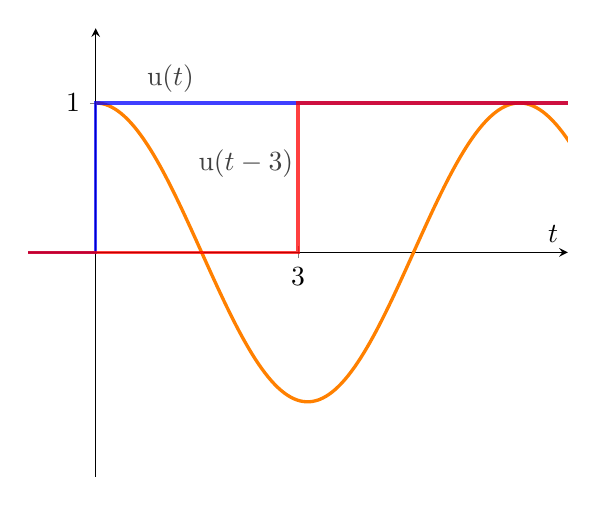
\begin{tikzpicture}
		\begin{axis}[%
		%    gray
		,xlabel=$t$
		%    ,ylabel=$u(t)$
		,axis lines = center
		,ymax=1.5
		,ymin=-1.5
		%    ,axis x line = bottom,axis y line = left
		,ytick={0,1}
		,xtick={0,3}
		% ,xticklabels={$0$,$\pi$}
		,xmin=-1
		,xmax=7
		%    ,ymax=1.2 % or enlarge y limits=upper
		%    ,xmin=-1.2
		]
		%\addplot+[const plot, no marks,thick,opacity=1] coordinates {(-1,0) (3.14,1) (7,1)} node[midway,anchor=east,black] {$b(t)$};
		\addplot[samples=200,very thick,color=orange,opacity=1,domain=0:3*pi] {cos(deg(x))};
		\addplot+[const plot, no marks,very thick,opacity=0.75,color=blue] coordinates {(-1,0) (0,1) (7,1)} node[pos=0.3,anchor=south,black] {$\mathrm u(t)$};
		\addplot+[const plot, no marks,very thick,color=red,opacity=0.75] coordinates {(-1,0) (3,1) (7,1)} node[right,pos=0.3,black] {$\mathrm u(t-3)$};
		%\addplot+[const plot, blue, no marks,very thick] coordinates {(-4,0) (1,1) (4,1)} node[below,pos=.57,black] {$u_c$};
		%\addplot+[const plot, no marks, thick] coordinates {(0,0) (1,0.25) (2,0.4) (3,0.5) (4,1) (4.49,1)} node[below=1.15cm,pos=.76,black] {$F_y$};
		\end{axis}
		\end{tikzpicture}
		~
		\begin{tikzpicture}
		\begin{axis}[%
		%    gray
		,xlabel=$t$
		%    ,ylabel=$u(t)$
		,axis lines = center
		,ymax=1.5
		,ymin=-1.5
		%    ,axis x line = bottom,axis y line = left
		,ytick={0,1}
		,xtick={0,3}
		% ,xticklabels={$0$,$\pi$}
		,xmin=-1
		,xmax=7
		%    ,ymax=1.2 % or enlarge y limits=upper
		%    ,xmin=-1.2
		]
		\addplot[samples=200,very thick,color=orange,opacity=1,domain=0:3] {cos(deg(x))};
		\addplot+[const plot, no marks,very thick,opacity=1,color=orange] coordinates {(3,-1) (3,0) (6.8,0)} node[midway,above,black] {$g(t)$};
		\end{axis}
		\end{tikzpicture}
		
	\end{centering}
	\begin{gather*}
	g(t) = \left[u(t)-u(t-\pi)\right]\sin t \\
	\implies g(t) = u(t)\sin t +u(t-\pi)\sin(t-\pi)\\
	\leftrightarrow \frac{1}{s^2+1}+e^{-\pi s}\frac{1}{s^2+1}
	\\
	Y(s) \overset{\text{13.2}}{=}\left(1+e^{-\pi s}\right)\frac{1}{(s^2+s+^5/_4)\left(s^2+1\right)}
	\\
	H(s) = \frac{1}{(s^2+s+^5/_4)\left(s^2+1\right)} = \frac{As+B}{s^2+s+^5/_4} + \frac{Cs+D}{s^2+1}
	\\
	\implies \begin{cases}
	A &= \frac{16}{17} \\
	B &= \frac{12}{17} \\
	C &= - \frac{16}{17} \\
	D &= \frac{4}{17}
	\end{cases} \implies H(s) = \frac{4}{17} \left[
	\frac{4s+3}{s^2+s+^5/_4}+ \frac{-4s+}{s^2+1}
	\right]
	\\
	s^2+s+^5/_4 = \left(s+\frac{1}{2}\right)^2 + 1 \\
	4s+3 = 4\left(s+\frac{1}{2}-\frac{1}{2}\right)+3 = 4\left(s+\frac{1}{2}\right)+1
	\\
	H(s) = \frac{4}{17} \left[
	4+\frac{s+^1/_2}{\left(s+^1/_2\right)^2+1}+\frac{1}{\left(s+\frac{1}{2}\right)^2+1}-4\frac{s}{s^2+1}+\frac{1}{s^2+1}
	\right] \leftrightarrow \\
	\leftrightarrow \frac{4}{17} \left[
	4e^{-\frac{t}{2}}\cos t + e^{-\frac{t}{2}}\sin t - 4\cos t +\sin t =h(t)
	\right] \\
	Y(s) = 
	\left(1+e^{-\pi s}\right)H(s) = H(s) + e^{-\pi s}H(s) \leftrightarrow h(t) + \mathrm u(t-\pi)h(t-\pi)
	\end{gather*}
\end{exercise*}

\subsection{Συνάρτηση δέλτα - \textlatin{Dirac}}
\begin{align*}
\mathrm{\delta}(t) =& \lim_{n\to \infty}\mathrm \delta_n(t),\ t \in \mathbb R, & \delta_n(t) = n \left[
\mathrm u(t) - u\left(t-\frac{1}{n}\right)
\right] \\
&
\left\lbrace \mathrm \delta_n \right\rbrace_{n=1}^\infty
& \mathrm{\delta}_n(t) = \begin{cases}
0 \quad& t\leq0 \\ n \quad& 0 \leq t < \frac{1}{n} \\ 0 \quad& t \geq \frac{1}{n}
\end{cases} \\ & & \mathrm \delta(t) = \begin{cases}
0 \quad& \text{για } t \neq 0\\
\infty \quad& \text{για } t = 0
\end{cases}
\end{align*}

\subsubsection{Συνάρτηση κρουστικής απόκρισης}
στο \( c \geq 0 \) \( \boxed{\mathbf L(y) = y''+a_1y'+a_0y_0} \)

με \( \mathbf L(y_\delta) = \delta (t-c) \)

\( \delta(t-c) \leftrightarrow e^{-cs} \quad c \geq 0 \)

\begin{exercise*}{13.4}
	Να βρεθεί η συνάρτηση της κρουστικής απόκρισης του τελεστή \( \mathbf L \)
	\[
	\mathbf L (y) = y''+2y'+2y
	\]
	\( t=0 \)
		\tcblower
	
	\( y_\delta(0) = 0,\ y_\delta'(0) = 0 \)

	
	\begin{gather*}
	\xrightarrow{\mathscr L}
	\left[
	s^2Y_\delta(s) - (0)s-(0)
	\right] + 2 \left[sY_\delta(s)-(0) \right] +2Y_\delta(s) = 1
	\\ \implies Y_\delta(s) = \frac{1}{s^2+2s+2} = \frac{1}{(s+1)^2+1} \implies \boxed{y_\delta(t) = e^{-t}\sin t}
	\end{gather*}
\end{exercise*}

\begin{exercise*}{13.5}
	\( t = c\geq0 \)


	\[
	L(y) = y''+2y'+2y
	\]
	
	\begin{gather*}
	y_\delta \ \text{Α.Τ.} y''_\delta + 2y_\delta' + 2y_\delta = \delta(t-c)
	\\ y_\delta(0) = 0, y_\delta'(0) = 0, c \geq 0 \\
	\xrightarrow{\mathscr L}
	s^2Y_\delta(s)+2sY_\delta(s)+2Y_\delta(s) = e^{-cs}
	\\ \implies Y_\delta(s) = \frac{e^{-cs}}{s^2+2s+2} = \frac{e^{-cs}}{(s+1)+1}
	\\ \implies \boxed{
		y_\delta(t) = \mathrm u(t-c)e^{-(t-c)}\sin (t-c)
		}
	\end{gather*}
\end{exercise*}


\begin{exercise*}{13.6}
	\[
	y''-y=-20\delta(t-3), \quad y(0) = 1,\ y'(0) = 0
	\]
	\tcblower
	\begin{gather*}
	\left[s^2Y(s)-s-0\right]-Y(s)=-20e^{-3s} \\
	\implies Y(s) = \frac{s}{s^2-1}-20e^{-3s}\frac{1}{s^2-1} \leftrightarrow \\
	\leftrightarrow \cosh(t)-20\mathrm u(t-3)\sinh(t-3)
	\end{gather*}
\end{exercise*}

\begin{exercise*}{13.7}
	\[
	y''+4y = \delta(t-\pi)-\delta(t-2\pi); \quad y(0) = 0,\ y'(0)=0
	\]
	\tcblower
	\begin{gather*}
	\left[s^2Y(s)\right]+4Y(s) = e^{-\pi s}-e^{-2\pi s}
	 \\
	 \implies Y(s) = \frac{e^{-\pi s}}{s^2+4} - \frac{e^{-2\pi s}}{s^2+4} = \frac{e^{-\pi s}}{2}\frac{2}{s^2+4}-\frac{e^{-2\pi s}}{2}\frac{2}{s^2+4}\\
	 \leftrightarrow \frac{1}{2}\mathrm u(t-\pi) \sin \left[2(t-\pi)\right]-\frac{1}{2}\mathrm u(t-2\pi)\sin\left[2(t-2\pi)\right]=y(t)
 \\
 y(t) = \frac{1}{2} \left[
 \mathrm u(t-\pi)-\mathrm u(t-2\pi)
 \right] \sin 2t
 	\end{gather*}
\end{exercise*}




























































\newpage

\part{Κεχαγιάς: Ολοκληρωτικοί μετασχηματισμοί}
\textlatin{(Fourier, Laplace)}
Τετάρτη 17:00-18:30

\section{Κεφάλαιο 7: Εισαγωγή στην ανάλυση του \text{Fourier}}
\begin{circuitikz} \draw
(0,0) to[american voltage source=$V$] (0,4)
      to[R=$R$] (4,4) 
      to[C=$C$] (4,0) -- (0,0);
\end{circuitikz}

H συμπεριφορά του κυκλώματος μπορεί να περιγραφεί με μια διαφορική εξίσωση.

\(Q(t)\): Το φορτίο του πυκνωτή σε χρονική στιγμή \(t\)

\begin{align*}
v_1 &= R\cdot i(t) = \frac{\dif Q}{\dif t}\\
v_2 &= \frac{Q(t)}{C} \\
&\boxed{v_1 + v_2 = V(t) \implies \frac{\dif Q}{\dif t} + \frac{Q(t)}{RC} = \frac{1}{R}V(t), \quad \text{με αρχική συνθήκη }Q(0)=0}
\end{align*}

Θα προσπαθήσω να λύσω την εξίσωση για τρεις περιπτώσεις:

\pgfplotsset{width=6.5cm}
\paragraph{}
\begin{tikzpicture}
  \begin{axis}[ 
    xlabel=$t$,
    ylabel={$V(t)$},
    axis lines=middle,
    xtick=\empty,
	ytick=\empty,
	title={$V(t)=V_0$}
  ] 
    \addplot[blue,thick,domain=0:5] {5}; 
  \end{axis}
\end{tikzpicture}
\hskip 10pt
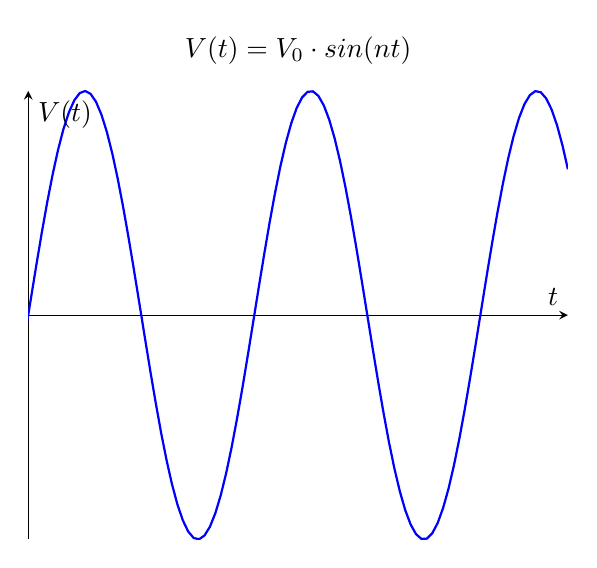
\begin{tikzpicture}
  \begin{axis}[ 
    xlabel=$t$,
    ylabel={$V(t)$},
    axis lines=middle,
    xtick=\empty,
	ytick=\empty,
	xmin=0,
	title={$V(t)=V_0\cdot sin(nt)$}
  ] 
    \addplot[blue,thick,samples=200] {5*sin(deg(3*x))}; 
  \end{axis}
\end{tikzpicture}
\hskip 10pt
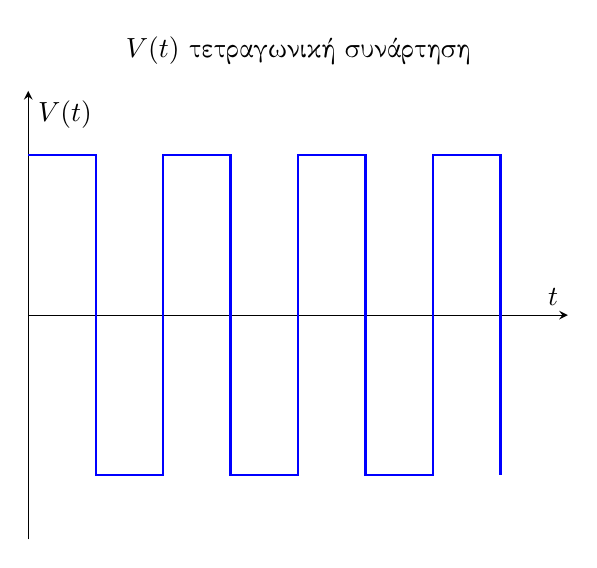
\begin{tikzpicture}
  \begin{axis}[ 
    xlabel=$t$,
    ylabel={$V(t)$},
    axis lines=middle,
    xtick=\empty,
	ytick=\empty,
	xmin=0,
	xmax=8,
	ymin=-1.4,
	ymax=1.4,
	title={$V(t)\text{ τετραγωνική συνάρτηση}$}
  ] 
    \addplot+[blue,thick,mark=none,const plot]
coordinates
{(0,1) (1,-1) (2,1) (3,-1) (4,1) (5,-1) (6,1) (7,-1)};
  \end{axis}
\end{tikzpicture}

\subsubsection{\(V(t) = V_0\)}
\[
\frac{\dif x}{\dif t}+ax=b
\]
Θα εξετάσω τη γενική λύση \(x_0(t)\) της ομογενούς ΔΕ, και \\
θα ψάξω μία ειδική λύση της μη ομογενούς ΔΕ.

Ομογενής: \(b=0 \implies \frac{\dif x}{\dif t} = -ax \implies x(t)=ce^{-at}.\)\\\(x(0)=0\implies c=0 \implies x_0(t)=0\).

Μη ομογενής: \(\frac{\dif x}{\dif t}+ax=b\).
\[
x(t)=k \implies \frac{\dif x}{\dif t}+ak=b \implies k =\frac{b}{a} \implies x(t)=k=\frac{b}{a}
\]

\begin{theorem*}{}
%\paragraph{Θ.}
Η γενική λύση της μη ομογενούς είναι:
\[x(t) = x_h(t)+x_i(t) \]
\end{theorem*}

Άρα \[
\begin{cases}
x(t) = ce^{-at} - \frac{b}{a} \\
x(0) = 0
\end{cases}
\implies 0=x(0)=c+\frac{b}{a}
\implies x(t) =\frac{b}{a}-\frac{b}{a}e^{-at} \text{ ή και }
 x(t) =\frac{b}{a}(1-e^{-at})
 \]

\begin{tikzpicture}
  \begin{axis}[ 
    xlabel=$t$,
    ylabel={$x(t)$},
    axis lines=left,
    xtick=\empty,
	ytick=\empty
  ] 
    \addplot[blue,thick,domain=0:5] {1-e^(-x)}; 
  \end{axis}
\end{tikzpicture}

 
\[
a=\frac{1}{RC}, \quad b= \frac{V_0}{R}
\]

\subsubsection{\(V(t)=V_0 \sin(nt)\)}
\[
\frac{\dif x}{\dif t} + ax = b\sin (nt)
\]

Είναι \(x_h(t) = ce^{-at}\).

Υποθέτω \(x(t) = c_2 \sin (nt) + c_3 \cos (nt) \). Τότε \( \frac{\dif x}{\dif t} = nc_2 \cos (nt) - nc_3 \sin (nt) \):

\[ \frac{\dif x}{\dif t} +ax =
\left( ac_2 - nc_3
\right)
\sin (nt) +
\left( ac_3 + nc_2
\right) \cos (nt)
= b \sin (nt) \implies
\]

\[
\implies
\begin{cases}
ac_2-nc_3&=b \\
nc_2+ac_3&=0 
\end{cases}
\implies \cdots \implies
\begin{cases}
c_2 &= \frac{ab}{a^2+n^2} \\
c_3 &= -\frac{bn}{a^2+n^2} 
\end{cases}
\]

Θυμάμαι ότι \(x(t) = x_h(t)+x_i(t) = c_1e^{-at} + \frac{ab}{a^2+n^2} \sin (nt) -  \frac{bn}{a^2+n^2} \cos (nt)\) και από το \(x(0)=0\) βρίσκω \(c_1 = \frac{bn}{a^2+n^2}\).

Άρα:
\[
x(t) = \frac{bn}{a^2+n^2} + \frac{ab}{a^2+n^2} \sin (nt) -  \frac{bn}{a^2+n^2} \cos (nt)
\]

Για το \(RC\) κύκλωμα, \(a=\frac{1}{RC} \leftarrow \) χρονική σταθερά κυκλώματος, \(b=\frac{V_0}{R}\), άρα:
\[
Q(t) = \frac{V_0C^2Rn}{C^2R^2n^2+1}e^{-\frac{t}{RC}} + \frac{CV_0\sin (nt) - C^2RnV_0 \cos (nt)}{C^2R^2n^2+1}
\]

\begin{attnbox}{}
\begin{align*}
p \cos (\omega t) + q \sin (\omega t) = \\
\sqrt{p^2+q^2} \left( \frac{p}{\sqrt{p^2+q^2}} \cos \omega t+ \frac{q}{\sqrt{p^2+q^2}} \sin \omega t \right) = \\
\sqrt{p^2+q^2} \left ( \sin \phi \cos \omega + \cos \phi \sin \omega t \right) = \\
\sqrt{p^2+q^2} \sin ( \omega t + \phi ), \quad \phi = \arctan \frac{p}{q}
\end{align*}
\end{attnbox}

Παρατηρούμε ότι ο πυκνωτής φορτίζει περισσότερο αν είναι μικρότερη η συχνότητα του εναλλασσόμενου ρεύματος.

\pgfplotsset{width=0.8\textwidth}
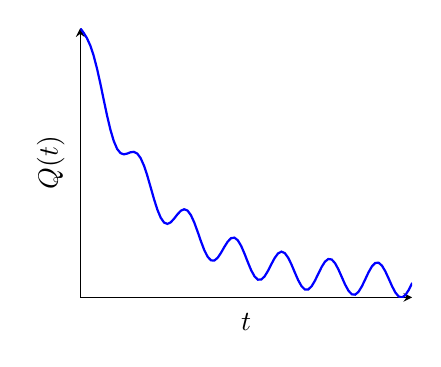
\begin{tikzpicture}
  \begin{axis}[ 
  	height=5cm,
    xlabel=$t$,
    ylabel={$Q(t)$},
    axis lines=left,
    xtick=\empty,
	ytick=\empty
  ] 
    \addplot[blue,samples=100,thick,domain=0:2*pi] {1.5*e^(-0.75*x)+0.1*sin(400*x)}; 
  \end{axis}
\end{tikzpicture}

\subsubsection{\(V(t) = \mathrm{square}(t)\)}
%\begin{tikzpicture}[domain=0:14]
%\draw (0,0) -- (0,4);
%\draw (0,4) -- (2,4);
%\draw (2,4) -- (2,0) node[anchor=west] {\(\pi\)};
%\draw (2,0) -- (2,-4) -- (4,-4) -- (4,4) -- (6,4) -- (6,-4);

%\draw[color=blue]
%plot (\x,{exp(-\x) + 0.35*sin(5*\x r)})
%node[right] {$f(x) = \sin x$};
%\end{tikzpicture}
\[
V(t)= \sum _{n = (1,3,5,\dots)} \frac{4}{n \pi} \sin (n t) =
\frac{4}{ \pi} \sin (n t) + \frac{4}{3 \pi} \sin (3 t) +
+ \frac{4}{5 \pi} \sin (5 t) \frac{4}{7 \pi} \sin (7 t) + \cdots
\]

Έτσι γίνεται η ανάλυση \textlatin{Fourier}, και αυτό θα το δούμε την επόμενη Τετάρτη, που θα πάμε στο Κεφάλαιο 8, που λέει σειρές \textlatin{Fourier}.

\[
V_N(t) = \sum _{n = (1,3,5,\dots)}^N \frac{4}{n \pi} \sin (n t)
\]
\[
V(t) = \sum _{n = (1,3,5,\dots)}^\infty \frac{4}{n \pi} \sin (n t) = \lim_{t \to \infty} V_N(t)
\]

\paragraph{}
Άρα:
\[
 \frac{\dif R}{\dif t}  + \frac{1}{RC}Q(t) = \frac{V_0 \sin (nt)}{R} \implies
 Q_n(t) = \frac{V_0C^2Rn}{C^2R^2n^2+1}e^{\frac{t}{RC}} + \frac{CV_0\sin (nt) - C^2RnV_0 \cos (nt)}{C^2R^2n^2+1}
\]

Οπότε αν:
\[
 \frac{\dif R}{\dif t}  + \frac{1}{RC}Q(t) = \frac{4}{\pi} \frac{\sin (nt)}{R} \implies
 Q_1(t) = \frac{4}{\pi} \left( \frac{C^2R}{C^2R^1+1} e^{-\frac{1}{RC}}+ \cdots \right)
\]
\[
 \frac{\dif R}{\dif t}  + \frac{1}{RC}Q(t) = \frac{4}{3\pi} \frac{\sin (3t)}{R} \implies
 Q_3(t) = \frac{4}{3\pi} \left( \frac{3C^2R}{9C^2R^1+1} e^{-\frac{1}{RC}}+ \cdots \right)
\]
\[
 \frac{\dif R}{\dif t}  + \frac{1}{RC}Q(t) = \frac{4}{5\pi} \frac{\sin (5t)}{R} \implies
 Q_5(t) = \cdots
\]

Άρα:
\[
Q(t) = \sum_{n \in \lbrace1,3,5,\dots\rbrace}Q_n(t)
\]

Γιατί όμως, αν \(V_1(t) \rightarrow Q_1(t), \ V_2(t) \rightarrow Q_2(t)\), τότε \(k_1V_1+k_2V_2 = k_1Q_1 +k_2Q_2\) σε αυτό το κύκλωμα (αρχή επαλληλίας/γραμμικότητα)?


\section{Σειρές \textlatin{Fourier}}

\begin{defn*}{}
Μία συνάρτηση \(f(t)\) λέγεται \textbf{τμηματικά συνεχής} στο \([t_1,t_2]\) ανν μπορώ να διαμερίσω:
\[ [t_1,t_2] = [\tau_0,\tau_1] \cup [\tau_1,\tau_2] \cup \cdots \cup [\tau_{n-1},\tau_n] \]
όπου \(\tau_0 = t_1,\ \tau_n = t_2\), τέτοια ώστε \(f(t)\) συνεχής στο κάθε \((\tau_{i-1},\tau_i)\), και υπάρχουν \(\lim_{t \to \tau_i^-} f(t),\ \lim_{t \to \tau_1^+}\ f(t) \forall i\)
\end{defn*}

\textit{π.χ}

\begin{center}
	\begin{tikzpicture}[scale=0.5]
	\draw[->] (-5,0) -- (11,0);
	\draw[->] (0,-5) -- (0,5);
	
	\draw[dashed] (-pi,0) -- (-pi,-1);
	\draw[dashed] (1*pi,-1) -- (1*pi,1);
	\draw[dashed] (2*pi,-1) -- (2*pi,1);
	\draw[dashed] (3*pi,0) -- (3*pi,1);
	
	\draw[thick,blue] (-pi, -1) -- (0,-1);
	\draw[thick,blue] (0,1) -- (pi,1);
	\draw[thick,blue] (pi,-1) -- (2*pi,-1);
	\draw[thick,blue] (2*pi,1) -- (3*pi,1);
	
	\filldraw[blue] (-pi,-1) circle (2.5pt);
	\filldraw[blue,fill=white] (0,-1) circle (2.5pt);
	\filldraw[blue] (0,1) circle (2.5pt);
	\filldraw[blue,fill=white] (pi,1) circle (2.5pt);
	\filldraw[blue] (pi,-1) circle (2.5pt);
	\filldraw[blue,fill=white] (2*pi,-1) circle (2.5pt);
	\filldraw[blue] (2*pi,1) circle (2.5pt);
	\filldraw[blue,fill=white] (3*pi,1) circle (2.5pt);
	\filldraw[blue] (3*pi,0) circle (2.5pt);
	
	\end{tikzpicture}
\end{center}


Η \(f(t)\) είναι τμηματικά συνεχής στο \([-\pi,3\pi]\), επειδή, για \(t_1=-\pi,t_2=3\pi\):
\[
[-\pi,3\pi] = [-\pi,0] \cup [0,\pi] \cup [\pi,2\pi] \cup [2\pi,3\pi]
\]
Στα \( (-\pi,0),\ (0,\pi) ,\   (\pi,2\pi) ,\   (2\pi,3\pi)\) η \(f\) είναι συνεχής, και υπάρχουν τα αντίστοιχα πλευρικά όρια
άρα η \(f\) είναι τμηματικά συνεχής.

\subsubsection{Συνθήκες του \textlatin{Dirichlet}}
\begin{enumerate}
\item Η \(f(t)\) είναι ορισμένη στο \((-L,L)\)
\item Η \(f(t)\) είναι τμηματικά συνεχής στο \((-L,L)\)
\item Η \(f(t)\) είναι περιοδική με περίοδο \(2L\).
\end{enumerate}

\subsection*{}

\begin{theorem*}{}
Έστω \(f(t)\) η οποία ικανοποιεί τις συνθήκες \textlatin{Dirichlet} στο \((-L,L)\). Τότε:
\begin{enumerate}
\item
Για κάθε σημείο συνέχειας της \(f(t)\):
\[
f(t) = \frac{a_0}{2}+\sum_{n=1}^\infty a_n \cos \frac{n\pi t}{L}
+\sum_{n=1}^\infty b_n \sin \frac{n\pi t}{L}
\]
όπου:
\begin{align*}
a_n&=\frac{1}{L} \int_{-L}^L f(t) \cos \frac{n\pi t}{L} \dif t \\
b_n&=\frac{1}{L} \int_{-L}^L f(t) \sin \frac{n\pi t}{L} \dif t
\end{align*}

\item Σε κάθε σημείο ασυνέχειας \(\tau\):
\[
\frac{1}{2} \left( \lim_{t \to \tau^-}f(t) + \lim_{t \to \tau^+}f(t) \right) 
= \frac{a_0}{2}+\sum_{n=1}^\infty a_n \cos \frac{n\pi t}{L}
+\sum_{n=1}^\infty b_n \sin \frac{n\pi t}{L}
\]
\end{enumerate}

\end{theorem*}

\paragraph{Παρ.}
\(f(t) = \text{τετραγωνικός παλμός}\)

\subparagraph{Λύση}
Η \(f(t)\) ικανοποιεί τις Σ.\textlatin{D} με \(L=\pi\)
\begin{align*}
a_0 &= \frac{1}{\pi} \int_{-\pi}^\pi f(t) \dif t = \frac{1}{\pi}\int_{-\pi}^0(-1)\dif t+\frac{1}{\pi}\int_{-\pi}^0 1\dif t = -1 + 1 = 0 \\
b_n &= \frac{1}{\pi} \int_{-\pi}^\pi f(t) \sin \frac{n \pi t}{\pi} \dif t
= \frac{2}{\pi} \int_0^\pi 1 \sin (nt) \dif t \\
&= \frac{2}{\pi} \cdot \left( \frac{-\cos nt}{n} \right)_{t=0}^\pi
=\frac{2}{\pi} \cdot \left( \frac{1-\cos n\pi}{\pi} \right) =
\frac{2}{\pi} \left( \frac{1-(-1)^n}{n} \right) = \frac{2}{n\pi} \text{ για άρτια }n
\end{align*}

Άρα:
\begin{align*}
a_0=a_1=a_2=\cdots=0 \\
b_1=\frac{4}{\pi}, \quad b_3=\frac{4}{3\pi} \\
\quad b_2=0, \quad b_4 = 0, \dots
\end{align*}
%a_n &= \frac{1}{\pi} \int_{-\pi)^\pi \underbrace{f(t)}_{\text{άρτια}} \underbrace{\cos \frac{n \pi t}{\pi}}_{\text{άρτια}}

\paragraph{Απόδειξη} (Μερική)

Θα δεχτούμε ότι η \(f(t)\) γράφεται στη μορφή \(f(t) = \frac{a_0}{2}+\sum_{n=1}^\infty a_n \cos \frac{n\pi t}{L}
+\sum_{n=1}^\infty b_n \sin \frac{n\pi t}{L}\),
και θα δείξουμε τους τύπους \(
a_n=\frac{1}{L} \int_{-L}^L f(t) \cos \frac{n\pi t}{L} \dif t ,\ 
b_n=\frac{1}{L} \int_{-L}^L f(t) \sin \frac{n\pi t}{L} \dif t
\)

Έστω \(f(t)= \frac{a_0}{2}+\sum_{n=1}^\infty a_n \cos \frac{n\pi t}{L}
+\sum_{n=1}^\infty b_n \sin \frac{n\pi t}{L}\).
Tότε: \[\int_{-L}^L f(t) \dif t = \int_{-L}^L f(t) \cdots t
= \int_{-L}^L \frac{a_0}{2} \dif t +
 \int_{-L}^L a_1 \cos \frac{\pi t}{L} \dif t +
 \int_{-L}^L a_2 \cos \frac{2\pi t}{L} + \cdots  = a_0\cdot L + 0 + 0 + \dots
\]
Άρα:
\[
a_0 = \frac{1}{L} \int_{-L}^L f(t) \dif t
\]

\subparagraph{Συνέχεια απόδειξης}
Υποθέτω ότι υπάρχει \textbf{κάποια} σειρά της μορφής *, θα δείξω ότι οι συντελεστές δίνονται από τους τύπους **.
ίό
Παρνω τυχόν \(m \in \mathbb N\) και εξετάζω το
\begin{align*}
\int_{-L}^L f(t) \cos \frac{m\pi t}{L} \dif t
&= \\ &=
\int_{-L}^L \left( \frac{a_0}{2}+\sum_{n=1}^\infty a_n \cos \frac{n\pi t}{L}
+\sum_{n=1}^\infty b_n \sin \frac{n\pi t}{L}\right)\cos \frac{m\pi t}{L} \dif t
\\ &=
\underbrace{\int_{-L}^L \frac{a_0}{2}\cos \frac{m\pi t}{L} \dif t}_{
=0\text{ ολοκληρώνω πάνω σε }m\text{ περιόδους}
}
+ \sum_{n=1}^\infty \int_{-L}^L a_n \cos \frac{n\pi t}{L} 
\cos \frac{m \pi t}{L} \dif t
+ \underbrace{\sum_{n=1}^\infty \int_{-L}^L b_n \sin \frac{n\pi t}{L} 
\cos \frac{m \pi t}{L} \dif t}_{
=\frac{b_n}{2} \left( \int_{-L}^L\sin\frac{n\pi t + m\pi t}{L} \dif t +
\int_{-L}^L\sin\frac{n\pi t - m\pi t}{L} \dif t
\right) = 0
}
\\ &=
 \sum_{n=1}^\infty a_n \int_{-L}^L \cos\frac{n\pi t}{L} \cos\frac{m\pi t}{L } \dif t
\\ & \overset{\cos a \cdot \cos \beta= \frac{\cos(a+\beta)+\cos(a-\beta)}{2}}{=} 
 \sum_{n=1}^\infty \frac{a_n}{2} \int_{-L}^L \left( \cos \frac{(n+m)\pi t}{L}
+ \cos \frac{(n-m)\pi t}{L}
\right) \dif t
\\ &=
 \sum_{n=1}^\infty \begin{cases}
0, \quad & n \neq m \\
a_nL, & n=m
\end{cases} \\
&= a_mL
\end{align*}

Επομένως:
\[
a_m = \frac{1}{L} \int_{-L}^L f(t) \cos \frac{n\pi t}{L} \dif  t
\]

Αντιστοίχως αποδεικνύεται και η σχέση για το \(b_m\).

Να σημειωθεί ότι οι συνθήκες του \textlatin{Dirichlet} είναι ικανές, αλλά όχι αναγκαίες.

\subsubsection{}
\begin{gather*}
f(t) = 
\sum_{-\infty}^\infty c_ne^{\frac{in\pi t}{L}} \\
c_n = \frac{1}{2L} \int_{-L}^L e^{-in\pi t}{L} \dif t
\end{gather*}

\paragraph{Απόδειξη}
\begin{align*}
f(t) = \frac{a_0}{2}+\sum_{n=1}^\infty a_n \cos \frac{n\pi t}{L}
+\sum_{n=1}^\infty b_n \sin \frac{n\pi t}{L} &=
\frac{a_0}{2} +
%\sum_{n=1)^\infty a_n \frac{e^{\frac{in\pi t}{L}}+e^{\frac{-in\pi t}{L}}}{2}
%+\sum_{n=1)^\infty b_n \frac{e^{\frac{in\pi t}{L}}-e^{\frac{-in\pi t}{L}}}{2i}
\\ &=
%\begin{align*}
\frac{a_0}{2}
+ \sum_{n=1}^\infty \cdots e^{\frac{in\pi t}{L}}
+ \sum_{n=1}^\infty \frac{a_n-ib_n}{2}
e^{\frac{in\pi t}{L}} +
+ \sum_{n=-1}^{-\infty} \frac{a_{-n}+ib_{-n}}{2}
e^{\frac{in\pi t}{L}}
\end{align*}

Άρα \[
f(t) = \sum_{n=-\infty}^\infty c_n e^{\frac{in\pi t}{L}}
\]

όπου: \[
c_n = \begin{cases}
\frac{a_n-ib_n}{2},\quad & n \in \mathbb Z^+ \\
\frac{a_{-n}+ib_{-n}}{2},\quad & n \in \mathbb Z^- \\
\frac{a_0+ib_0}{2},\quad & n=0
\end{cases}
\]

Αφήνεται ως άσκηση για τον αναγνώστη να αποδειχθεί ότι:
\[
c_n =
\frac{1}{2L}
\int_{-L}^L f(t) e^{\frac{-in\pi t}{L}} \dif t
\]

\subsection{Παράδειγμα}
\begin{center}
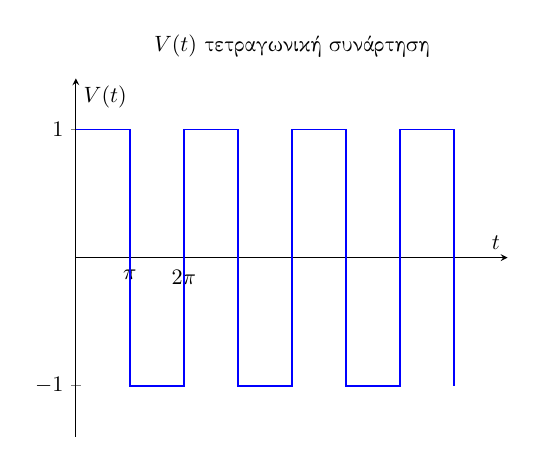
\begin{tikzpicture}[scale=0.8]
  \begin{axis}[ 
    xlabel=$t$,
    ylabel={$V(t)$},
    axis lines=middle
   ,ytick={-1,0,1}
   ,xtick={0,1,2}
   ,xticklabels={$0$,$\pi$,$2\pi$}
   ,yticklabels={$-1$,$0$,$1$},
	xmin=0,
	xmax=8,
	ymin=-1.4,
	ymax=1.4,
	title={$V(t)\text{ τετραγωνική συνάρτηση}$}
  ] 
    \addplot+[blue,thick,mark=none,const plot]
coordinates
{(0,1) (1,-1) (2,1) (3,-1) (4,1) (5,-1) (6,1) (7,-1)};
  \end{axis}
\end{tikzpicture}
\end{center}

Θα βρω την \textbf{εκθετική} σειρά της \(f(t)\).

\begin{align*}
c_n &= \frac{1}{2\pi}
\int_{-\pi}^\pi f(t)e^{-int}\dif t \\
&=
\frac{1}{2\pi}
\int_{-\pi}^0(-1)\cdot e^{-int} \dif t
+
\int_{0}^{\pi}1\cdot e^{-int} \dif t
\\ &=
\frac{1}{2\pi}
\left(
- \int_{-\pi}^0e^{-int}\dif t
+ \int_0^\pi e^{-int} \dif t
\right)
\\ &=
\frac{1}{2\pi}
\left(
 \left. \frac{e^{-int}}{in} \right|_{-\pi}^0
+ \left. \frac{e^{-int}}{in} \right|_0^\pi
\right)
\\ &=
\frac{1}{2\pi} \left(
\frac{1}{in} - \frac{e^{-in\pi}}{in} - \frac{e^{-in\pi}}{in} + \frac{1}{in}
\right)
\\ &=
\frac{1}{2\pi}
\left(
\frac{2}{in}
- \frac{2\cos (n \pi)}{in}
\right)
\\ c_n &=
\frac{i}{n\pi}
\cdot \big(
1-\cos n\pi
\big)
\end{align*}

\[
\begin{array}{r|l}
n & c_n \\
-2 & 0 \\
-1 & \frac{2i}{\pi} \\
0 & 0 \\
1 & \frac{-2}{\pi} \\
2 & 0 \\
3 & \frac{-2i}{3\pi}
\end{array}
\]

Άρα:

\[
f(t) = \cdots + \frac{2i}{3\pi} e^{i3t} + \frac{2i}{\pi} e^{-it}
- \frac{2i}{\pi} e^{it}
- \frac{2i}{3\pi} e^{i3t} + \cdots
\]

Ερωτήματα για τον αναγνώστη:
\begin{enumerate}
\item
Πότε έχει η τριγωνομετρική σειρά μόνο ημίτονα/μόνο συνημίτονα?
\item
Πότε έχει η εκθετική σειρά μόνο πραγματικούς/μόνο εκθετικούς όρους?
\end{enumerate}

\subsection{}
\begin{defn*}{}
Συμβολίζω με \(\mathfrak{F}_L\) το σύνολο των συναρτήσεων που ικανοποιούν τις συνθήκες \textlatin{Dirichlet} (με ημιπερίοδο \(L\))
\end{defn*}

\begin{theorem*}{}
Το \(\mathfrak F_L\) είναι διανυσματικός χώρος. 
\end{theorem*}
\paragraph{Απόδειξη}

Έστω \(f,g \in \mathfrak F_L\) και \(\kappa,\lambda \in \mathbb C\). Θα δείξω ότι \(\kappa f + \lambda g \in \mathfrak F_L\).

\subparagraph{Πράγματι}
\begin{enumerate}
\item
Αν οι \(f,g\) είναι ορισμένες στο \([-L,L]\) τότε και η \(\kappa f + \lambda g\) είναι ορισμένη στο \([-L,L]\).
\item
\begin{align*}
(\kappa f + \lambda g)(t+2L) &= \kappa f (t+2L) + \lambda g (t+2L) \\
&= \kappa f(t) + \lambda g(t) \\
&= (\kappa f + \lambda g)(t)
\end{align*}
Άρα η \(\kappa f + \lambda g\) έχει περίοδο \(2L\).

\item
Αν η \(f\) και η \(g\) είναι τμ. συνεχείς στο \([-1,1]\), τότε και η \(\kappa f+\lambda g\) είναι τμ. συνεχείς.
\end{enumerate}

Από τα 1,2,3, η \(\kappa f + \lambda g \in \mathfrak F_L\).

\begin{theorem*}{}
Το σύνολο \(  \left\lbrace e^{\frac{in\pi t}{L}} \right\rbrace^\infty_{-\infty} \) είναι μια ορθογώνια βάση του \(\mathfrak F_L\).
\tcblower
\paragraph{Δηλαδή}
κάθε \(f(t) \in \mathfrak{F}_L\) μπορεί να γραφεί:
\[
f(t) =
\sum_{n=-\infty}^\infty c_n e^{\frac{in\pi t}{L}}
\]

Επιπλέον \(\forall n,m,\ m \neq n\ e^{\frac{in\pi t}{L}} \perp e^{\frac{im\pi t}{L}}\)

Δηλαδή:
\[
e^{\frac{im\pi t}{L}} \cdot
e^{\frac{in\pi t}{L}} = 0
\]

Δηλαδή:
\[
\int_{-L}^L e^{\frac{im\pi t}{L}} \cdot
 e^{\frac{in\pi t}{L}} \dif t =0
\]

Για να ορίσω το εσωτερικό γινόμενο, θέλω \(
\|\vec{x}\|^2 = \vec{x} \cdot \vec{x} = \sum_n x_n\bar{x_n} = \sum(x_n)^2
\)

\[
f \cdot g = \int_{-L}^L f(t) \overline{g(t)} \dif t
\]

Άρα
\[
e^{\frac{im\pi t}{L}} \cdot
e^{\frac{in\pi t}{L}} =
\int_{-L}^L e^{\frac{im\pi t}{L}} e^{\frac{in\pi t}{L}} \dif t =
\int_{-L}^L e^{\frac{i(m-n)\pi t}{L}} \dif t =
\begin{cases}
2L, \quad & m=n \\
0, \quad & m \neq n
\end{cases}
\]

\end{theorem*}

\begin{itemize}
\item \(\mathfrak F_L\) το σύνολο των συναρτήσεων που ικανοποιούν \textlatin{Dirichlet}
\item Το \(\mathfrak F_L\) είναι ΔΧ
\item Το \(  \left\lbrace e^{\frac{in\pi t}{L}} \right\rbrace_{n \mathbb Z}\) είναι μια ορθογώνια βάση του \(\mathfrak{F_L}\)
\item Το \(  \left\lbrace \cos{\frac{in\pi t}{L}} \right\rbrace_{n =0}^{\infty} \cup \left\lbrace \sin{\frac{in\pi t}{L}} \right\rbrace_{n =1}^\infty\) είναι μια ορθογώνια βάση του \(\mathfrak{F_L}\)
\item \(\underbrace{f(t)}_{\mathclap{\text{περιοδική, με ημιπερίοδο $L$}}} = \sum_{n=-\infty^\infty} c_n e^\frac{in\pi t}{L}\), με
\[
c_n = \frac{1}{2L} \int_{-L}^L f(t)e^\frac{in\pi t}{L} \dif t
\]
\end{itemize}

\begin{center}
	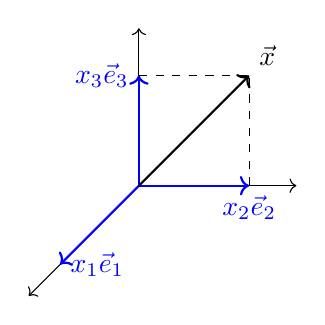
\begin{tikzpicture}[scale=2]
	\draw[->] (0,0) -- (0,1);
	\draw[->] (0,0) -- (1,0);
	\draw[->] (0,0) -- (-0.7,-0.7);
	
	\draw[blue,thick,->] (0,0) -- (0,0.7) node[left] {$x_3 \vec e_3$};
	\draw[blue,thick,->] (0,0) -- (0.7,0) node[below] {$x_2 \vec e_2$};
	\draw[blue,thick,->] (0,0) -- (-0.5,-0.5) node[right] {$x_1 \vec e_1$};
	\draw[dashed] (0.7,0) -- (0.7,0.7);
	\draw[dashed] (0,0.7) -- (0.7,0.7);
	\draw[thick,->] (0,0) -- (0.7,0.7) node[above right,sloped] {$\vec x$};
	
	\end{tikzpicture}
\end{center}
\begin{align*}
\vec{x} = [x_1 x_2 x_3] &= x_1 \vec{e_1} +x_2 \vec{e_2}+x_3 \vec{e_3}
\\ &=
\mathrm{Proj}(\vec{x}, \vec{e_1})
+\mathrm{Proj}(\vec{x}, \vec{e_2})
+ \mathrm{Proj}(\vec{x}, \vec{e_3})
\\ &=
\sum_{n=1}^3
\vec{x} \cdot \vec{e_n} \cdot \frac{\vec{e_n}}{\norm{\vec{e_n}}}
\end{align*}

Άρα:
\[
f(t) = \sum_{n=-\infty^\infty} c_n e^\frac{in\pi t}{L}
= \sum_{n=-\infty^\infty} \mathrm{Proj} \left( f(t), e^\frac{in\pi t}{L} \right)
\]
όπου \(\mathrm{Proj} \left( f(t), e^\frac{in\pi t}{L} \right) =
f(t)\bullet e^\frac{in\pi t}{L} \frac{e^\frac{in\pi t}{L}}{\norm{e^\frac{in\pi t}{L}}}
\)

\begin{align*}
f(t) \bullet e^\frac{in\pi t}{L} &= \int_{-L}^L f(t) \cdot \overline{e^\frac{in\pi t}{L}} \dif t 
\\
\norm{e^\frac{in\pi t}{L}} &= \int_{-L}^L e^\frac{in\pi t}{L} \cdot e^\frac{-in\pi t}{L} \dif t = 2L
\end{align*}

\begin{theorem}{\textlatin{Plancherel}}{}
\[
\frac{1}{2L} \int_{-L}^L f(t) \overline{g(t)} \dif t =
\sum_n c_n \overline{r_n}
\]

Η \(\begin{cases}
f(t)&= \sum_n c_n e^\frac{in\pi t}{L} \\
f(t)&= \sum_n r_n e^\frac{in\pi t}{L}
\end{cases}\)
\end{theorem}

\paragraph{Απόδειξη}
\begin{align*}
\frac{1}{2L} \int_{-L}^L f(t) \overline{g(t)} \dif t &=
\frac{1}{2L} \int_{-L}^L 
	\left( \sum_{n=-\infty}^\infty c_n e^\frac{in\pi t}{L}
	\right)
	\overline{\left(
	\sum_{m=-\infty}^\infty c_m e^\frac{im\pi t}{L}
	\right)}
	\dif t
\\ &=
\frac{1}{2L} \int_{-L}^L \left(
\sum_{n=-\infty}^\infty \sum_{m=-\infty}^\infty
c_n e^\frac{in\pi t}{L}
\overline{r_m} e^\frac{im\pi t}{L} \right) \dif t
\\ &=
\frac{1}{2L}
\sum_{n=-\infty}^\infty
\sum_{m=-\infty}^\infty
c_n \bar{r_m}
\underbrace{\int_{-L}^L
e^\frac{i(n-m)\pi t}{L} \dif t}_{
\begin{cases}
0 \qquad & m \neq n\\
2L & m = n
\end{cases}
}
\\ &= \frac{1}{2L} 2L \sum_n c_n\bar{r_n}
\end{align*}

Γενικά:
\[
f(t) \leftrightarrow \vec{c} = [ \dots \ c_{-1}\  c_0\  c_1\ c_2\ \dots ]
\]
(με την επιφύλαξη ότι σε πεπερασμένο αριθμό σημείων μπορεί να αλλάζει η τιμή της συνάρτησης)

Σύμφωνα με το θεώρημα:
\begin{align*}
f(t) &\leftrightarrow \vec{c} \\
g(t) &\leftrightarrow \vec{r} \\
 \frac{1}{2L} f\bullet g &= \vec{c} \bullet \vec{r}
\end{align*}

\begin{theorem}{Πόρισμα (\textlatin{Parseval})}{}
\[
\frac{1}{2L} \int_{-L}^L
\left|
f(t)
\right|^2 \dif t
= \sum_n
|c_n|^2
\]
\begin{center}
	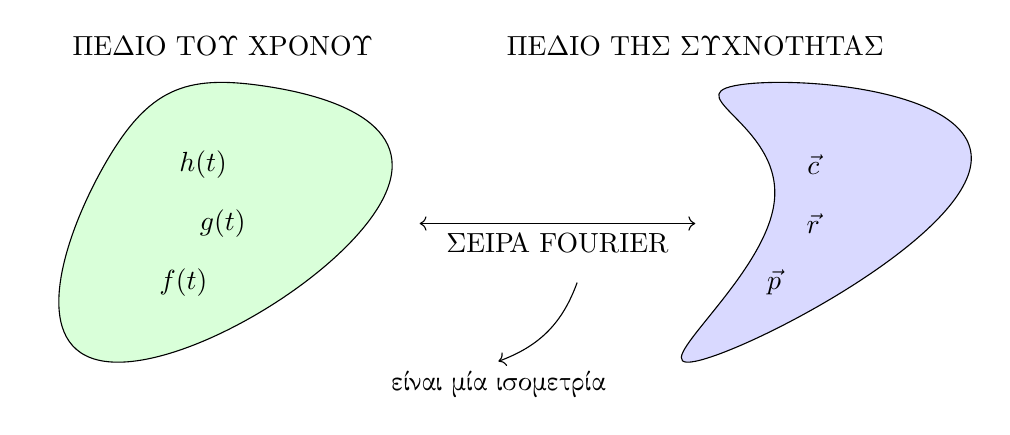
\begin{tikzpicture}[scale=5]
	\filldraw[fill=green!15] plot [smooth cycle,tension=1] coordinates {
		(0,0) (0,0.5) (0.4,0.7) (0.7,0.4)
	};		
	\draw (0.2,0.2) node {$f(t)$};
	\draw (0.3,0.35) node {$g(t)$};
	\draw (0.25,0.5) node {$h(t)$};
	\draw (0.3,0.8) node {ΠΕΔΙΟ ΤΟΥ ΧΡΟΝΟΥ};
	
	\begin{scope}[shift={(1.5,0)}]
	\filldraw[fill=blue!15] plot [smooth cycle,tension=1] coordinates {
		(0,0) (0.2,0.4) (0.1,0.7) (0.7,0.5)
	};
	\draw (0.2,0.2) node {$\vec p$};
	\draw (0.3,0.35) node {$\vec r$};
	\draw (0.3,0.5) node {$\vec c$};
	\draw (0,0.8) node {ΠΕΔΙΟ ΤΗΣ ΣΥΧΝΟΤΗΤΑΣ};
	
	\end{scope}
	
	\draw[<->] (0.8,0.35) -- (1.5,0.35) node[midway,below] {ΣΕΙΡΑ \textlatin{FOURIER}};
	
	\draw[->] (1.2,0.2) to [bend left=25] (1,0) node[below] {είναι μία ισομετρία};
	
	\end{tikzpicture}
\end{center}
\end{theorem}

\begin{theorem}{}{}
Αν \(f(t) \in \mathfrak F_L\) και \(f(t) = \sum_n c_n e^\frac{in\pi t}{L}\), τότε:
\begin{align*}
\od{f}{t}&=\sum_n c_n \frac{in\pi}{L} e^\frac{in\pi t}{L} \\
\int f(t)&=\sum_n c_n \frac{L}{in\pi} e^\frac{in\pi t}{L}
\end{align*}

Τα ίδια για ημίτονα και συνημίτονα
\end{theorem}

\paragraph{Παράδειγμα}
Δίνεται η \(f(t)
= \begin{cases}
|t| &\qquad t \in [-\pi,\pi] \\
\text{περιοδική επέκταση} &\qquad t \notin [-\pi,\pi]
\end{cases}
\)

Να βρεθεί η Σειρά (\textlatin{Fourier}) της \(f(t)\).
\subparagraph{Λύση}

\begin{center}
	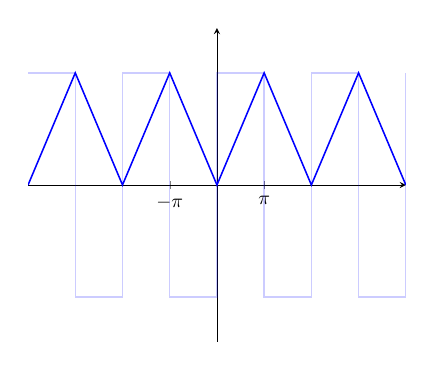
\begin{tikzpicture}[scale=0.7]
	\begin{axis}[ 
	%    xlabel=$t$,
	axis lines=middle
	,ytick={-1,0,1}
	,ytick={0}
	,xtick={0,3.14159,-3.14159}
	,xticklabels={$0$,$\pi$,$-\pi$}
	,yticklabels={$-\pi$,$0$,$\pi$},
	xmin=-4*pi,
	xmax=4*pi,
	ymin=-1.4,
	ymax=1.4,
	] 
	\addplot+[blue,thick,mark=none]coordinates{
		(-4*pi,0) (-3*pi,1) (-2*pi,0) (-1*pi,1) (0*pi,0) (1*pi,1) (2*pi,0) (3*pi,1) (4*pi,0)
	};
	\addplot+[blue,thick,mark=none,const plot,opacity=0.2]coordinates{
		(-4*pi,1) (-3*pi,-1) (-2*pi,1) (-1*pi,-1) (0*pi,1) (1*pi,-1) (2*pi,1) (3*pi,-1) (4*pi,1)
	};
	\end{axis}
	\end{tikzpicture}
\end{center}

Παρατηρώ ότι \( f(t) = \int g(t)\dif t \), όπου \( g(t) = \begin{cases}
1 \quad& t \in (0,\pi) \\
-1 \quad & t \in (-\pi,0]
\end{cases} \)

Αφού λοιπόν \(g(t)=
\frac{4}{\pi} \cdot
\left(
\sin t + \frac{\sin(3t)}{3} + \frac{\sin(5t)}{5} + \dots
\right)
\), τότε:
\begin{align*}
f(t) &=
c - \frac{4}{\pi}
\left(
\cos t + \frac{\cos 3t}{3^2}
+ \frac{\cos 5t}{5^2}
\right)
\\ f\left(\frac{\pi}{2}\right) &= \frac{\pi}{2} = c
\end{align*}

Άρα τελικά:
\[
f(t) = \frac{\pi}{2} - \frac{4}{\pi}
\left(
\cos t + \frac{\cos 3t}{3^2}
+ \frac{\cos 5t}{5^2}
\right)
\]

Παρατηρώ ότι η \(f\) έχει ασθενέστερες υψηλές συχνότητες από τη \(g\).

\paragraph{Παράδειγμα}
Να υπολογιστεί το:
\[
S_1 = 1 - \frac{1}{3} + \frac{1}{5} - \frac{1}{7} + \frac{1}{9} + \cdots
\]

Είναι \begin{align*}
g\left( \frac{\pi}{2}\right) &=
\frac{4}{\pi}\left(
\sin \frac{\pi}{2}+\frac{\sin\frac{3\pi}{2}}{3}
+ \frac{\sin\frac{5\pi}{2}}{5}
\right)
\\ 
1 = g\left( \frac{\pi}{2}\right) &= \frac{4}{\pi}
\left(
1-\frac{1}{3}+\frac{1}{5}-\cdots
\right) = S_1
\end{align*}

\paragraph{Παράδειγμα}
Να υπολογιστεί το:
\[
S_1 = 1 + \frac{1}{3^2} + \frac{1}{5^2} + \frac{1}{7^2} + \cdots
\]
\subparagraph{Λύση}
\begin{align*}
0=f(0)&=\frac{\pi}{2} - \frac{4}{\pi} \cdot\left(
1+\frac{1}{3^2}+\frac{1}{5^2}+\cdots
\right)
\\ \frac{\pi^2}{8} &= 1 + \frac{1}{3^2} + \frac{1}{5^2} + \cdots
\end{align*}




\section{Κεφάλαιο 9: Μετασχηματισμός \textlatin{Fourier}}
%TODO Kehagias Graph 04
\begin{theorem*}{}
Έστω ότι η \(f(t)\) ικανοποιεί τα εξής:
\begin{enumerate}
\item Τις συνθήκες \textlatin{Dirichlet} \(\forall L \in  \mathbb R \)
\item \( \int_{-\infty}^\infty |f(t)| \dif t < \infty\) (δηλ. η \(f(t)\) είναι απολύτως ολοκληρώσιμη)
\end{enumerate}

Τότε:
\[
f(t) = \frac{1}{2\pi}
\int_{-\infty}^\infty F(\omega) e^{i\omega t} \dif t
\]
όπου:
\[
F(\omega) = \int_{-\infty}^\infty f(t)e^{-i\omega t} \dif t
\]

\end{theorem*}

\paragraph{Απόδειξη}
Δίνεται η \(f(t)\). Διαλέγω τυχόν \(t\) και ορίζω την \(f_T(t) = f(t)\quad \forall t \in \left[ -\frac{T}{2}, \frac{T}{2} \right]\), που έχει σειρά \textlatin{Fourier}:
\[
f_T(t) = \sum_{n=-\infty}^\infty c(n) e^\frac{in2\pi t}{T}
\]
όπου
\[
c(n) = \frac{1}{T} \int_{-\frac{T}{2}}^\frac{T}{2} f(t) e^{-\frac{in2\pi t}{T}} \dif t
\]

Θέτω \(\delta \omega = \frac{2\pi}{T},\ \omega = n\cdot \delta \omega = \frac{2n\pi}{T}
\)

\begin{align*}
f_T(t) &= \sum_{n=-\infty}^\infty
\left(
\frac{1}{T} \int_{-\frac{T}{2}}^\frac{T}{2} f(t) e^{-\frac{in2\pi t}{T}} \dif t
\right) e^\frac{in2\pi t}{T}
\\ &= \frac{1}{2\pi}
\sum_{n=-\infty}^\infty
\left(
\frac{2\pi}{T}
\int_{-\frac{T}{2}}^\frac{T}{2}
f_T(t)e^{-i\omega t} \dif t
\right) e^\frac{in2\pi t}{T}
\\ &=
\frac{1}{2\pi}
\sum_{n=-\infty}^\infty
\left(
\int_{-\frac{T}{2}}^\frac{T}{2}
f_T(t)e^{-i\omega t} \dif t
\right)
e^{i\omega t} \delta \omega
\\ &=
\frac{1}{2\pi}
\int_{-\infty}^\infty
\underbrace{\left(
\int_{-\infty}^\infty
f(t)e^{i\omega t} \dif t
\right)}^{F(\omega)}
e^{i\omega t}
\dif \omega
\end{align*}

Την \(F(\omega)\) την ονομάζουμε \textbf{\textlatin{Fourier} μετασχηματισμένη} της \(f(t)\), και γράφουμε:
\[
\mathscr{F}\bigg( f(t) \bigg) = F(\omega)
\]

\begin{tcolorbox}
\[
F(\omega) = \mathscr{F} f(t)
\quad
f(t) = \mathscr{F}^{-1} \left( F(\omega) \right)
\]
\end{tcolorbox}

\paragraph{Παρ.}
\[
f(t)=
\begin{cases}
1 \quad |t|<a\\
0 \quad |t|\geq a
\end{cases}
\]

\begin{align*}
F(\omega) = \int_{-\infty}^\infty f(t)e^{-i\omega t} \dif t
&= \int_{-a}^a 1 e^{-i \omega t} \dif t = -\frac{1}{i \omega } e^{-i \omega t} \dif t
\\
&=
\frac{2}{\omega}
\left(
\frac{-e^{-i \omega a}}{2i}
\right)
\\ &= 2 \frac{\sin( \omega a)}{\omega}
\end{align*}

\paragraph{Παρ.}
\[
f(t)=e^{-|t|}
\]

\begin{align*}
F( \omega )&=\int_{- \infty }^ \infty e^{-|t|} e^{-i \omega t} \dif t
\\ &=
\int_{- \infty }^0 e^t e^{-i \omega t} \dif t
+ \int_0^ \infty e^{-t}e^{-i \omega t} \dif t
\end{align*}

\begin{align*}
\int_0^ \infty e^{-t}e^{-i \omega t} \dif t &=
-\left. \frac{1}{1+i\omega} \right|_{t=0}^\infty
\\
&= -\frac{1}{1+i\omega} \left(
e^{-(1+i \omega )\cdot\infty}-e^{-(1+i \omega )\cdot0}
\right)
\\ &=
-\frac{1}{1+i\omega}
\Bigg(
0-1
\Bigg)
\\ &= \frac{1}{1+i\omega}
\end{align*}


Άρα:
\begin{align*}
\int_{- \infty }^0 e^t e^{-i \omega t} \dif t
+ \int_0^ \infty e^{-t}e^{-i \omega t} \dif t
&= \frac{1}{1-i \omega }+\frac{1}{1+i \omega }\\
&=
\boxed{
\frac{2}{1+\omega^2} = \mathscr{F} \left(
e^{-|t|}
\right)
}
\end{align*}

\begin{tcolorbox}
Ο Μ/Σ \textlatin{Fourier} εφαρμόζεται μόνο σε απόλυτα ολοκληρώσιμες \(f(t)\). Δηλαδή υποθέτω ότι \[
\int_{- \infty }^ \infty 
\left|
f(t)
\right|
\dif t = M <  \infty 
\]

Αυτό το κάνω, διότι \(\int_{- \infty }^ \infty |f(t)| \dif t < M < \infty\) είναι ικανή συνθήκη για να υπάρχει το \(\int_{- \infty }^ \infty f(t)e^{-i\omega t}\).

Έχει μία σημαντική συνέπεια:
\[
\lim_{t\to\pm\infty} f(t) = 0
\]

Για παράδειγμα, οι \(\mathscr{F}(e^t)\) και \(\mathscr{F}(e^{-t})\) δεν υπάρχουν, ενώ ο \(\mathscr{F}(e^{-|t|})\) υπάρχει διότι η \(e^{-|t|}\) είναι απόλυτα ολοκληρώσιμη.

Επίσης \( \int_{-\infty}^ \infty |F(\omega)| \dif \omega = M' < \infty \)
\end{tcolorbox}

\begin{theorem}{}{}
\[
\mathscr{F}(\kappa f + \lambda g) = \kappa \mathscr{F}(f)+\lambda \mathscr{F}(g)
\]
\tcblower
\paragraph{Παρ.}
\[
 \mathscr{F} (3\cdot \mathrm{square} + 5\cdot e^{-|t|}) = 6 \frac{\sin(\omega)}{\omega}+\frac{10}{1+\omega^2}
\]
\end{theorem}
Η απόδειξη είναι εύκολη και αφήνεται για τον αναγνώστη.

\begin{attnbox}{}
Το \textlatin{Wolfram} επιστρέφει τους Μ/Σ \textlatin{Fourier} με διαφορετικό παράγοντα, για λόγους συμμετρίας! (\(\frac{1}{\sqrt{2\pi}}\) έναντι \(\frac{1}{2\pi}\)). Στις σημειώσεις τηρείται η ιστορική σύμβαση που ακολουθείται και από προγράμματα όπως, π.χ. \textlatin{Matlab}.
\end{attnbox}

\begin{theorem}{}{}
Έστω \(F( \omega )= \mathscr{F} \left( f(t) \right)\), τότε:
\[
 \mathscr{F} \left( F(t) \right) = 2\pi f(-\omega)
\]

Δηλαδή:
\[
 \mathscr{F} \left(  \mathscr{F} \left( f(t) \right) \right) = 2\pi f(-t)
\]
\end{theorem}
\paragraph{Απόδ.}
\begin{align*}
 \mathscr{F} \left( f(t) \right) = F(\omega) = \int_{-\infty}^\infty f(t)e^{-i\omega t} \dif t \\
 \mathscr{F}^{-1} \left( F(\omega)) \right) = f(t) = \frac{1}{2\pi}\int_{-\infty}^\infty F(\omega)e^{i\omega t} \dif \omega \\
 2\pi f(-t) = \int_{-\infty}^ \infty F(\omega) e^{-i\omega t} \dif \omega
 \\
= \int_{-\infty}^ \infty F(\tau)e^{-i\tau w} \dif \tau = 2\pi f(-w) \\
=  \mathscr{F} \left( F(\tau) \right) =2\pi f(-w)
\end{align*}

\paragraph{Παρ.}
\[
 \mathscr{F} \left(
 \frac{1}{1+t^2}
 \right)
\]
\subparagraph{Λύση}
\[
\dots = \int_{-\infty}^\infty \dots
\]
ή

Παρατηρώ ότι \( \mathscr{F} (\frac{1}{2}e^{-|t|}) = \frac{1}{1+\omega^2} = F(\omega) = F(-\omega)\)

Άρα \(F(t) = \frac{1}{1+t^2}\)
\[
 \mathscr{F}  \left(
 \frac{1}{1+t^2}
 \right) =  \mathscr{F} \left( F(t) \right) = 2\pi f(-\omega) = \pi e^{-|\omega|}
\]

\begin{theorem}{}{}
\[
 \mathscr{F} \left( f(at) \right) = \frac{1}{a} F \left(\frac{\omega}{a} \right)
\]
\end{theorem}
\paragraph{Απόδ.}
\begin{align*}
 \mathscr{F} \left( f(at) \right)&=\int_{-\infty}^\infty f(at) e^{-i  \omega t} \dif t
 \\ &=
 \int_{-\infty}^\infty f(at)e^{-i\frac{\omega}{a}at} \dif t
 \\ &=
\frac{1}{a}  \int_{-\infty}^\infty f(at)e^{-i\frac{\omega}{a}at} \dif (at)
=
\frac{1}{a} \int_{-\infty}^\infty f(\kappa) e^{-i\frac{\omega}{a}\kappa} \dif \kappa
= \frac{1}{a}	F\left( \frac{\omega}{a}\right)
\end{align*}

\paragraph{Παρ.}
\[
 \mathscr{F} \left( \frac{1}{4+9t^2} \right)
 = \frac{1}{4} \mathscr{F} \left( \frac{1}{1+\frac{9}{4}t^2} \right) 
 = \frac{1}{4}  \mathscr{F} \left( \frac{1}{1+\left(\frac{3}{2}t\right)^2} \right)
\]

Για \(f(t) = \frac{1}{1+t^2}, \quad F(\omega) = \pi e^{-|\omega|}\),
\[
f(\frac{3}{2}t = \frac{1}{1+\frac{9}{4}t^2} \rightarrow
\frac{1}{a} F\left(\frac{\omega}{a}\right) = \frac{2\pi}{3} e^{-\left|\frac{3\omega}{2}\right|}
\]

Άρα ο ζητούμενος μετασχηματισμός είναι \(
\frac{1}{4} \frac{2\pi}{3} e^{-\left|\frac{3\omega}{2}\right|}
\)

%TODO Kehagias 01

\begin{theorem*}{}
Έστω \(F(\Omega) = \mathscr{F}(f(t))\). Τότε
\begin{enumerate}
\item \(\mathscr{F}\left(\od{f}{t}\right) = i\omega F(\omega)\)
\item \(\mathscr{F}\left(\int f(t)\dif t\right) = \frac{1}{i\omega}F( \omega )\)
\item \(\mathscr{F}\left(-itf(t)\right) = \od{F}{\omega}\)
\end{enumerate}
\end{theorem*}
\paragraph{Απόδ.}
\begin{align*}
\mathscr{F}\left(\od{f}{t}\right) &= \int_{-\infty}^\infty \od{f}{t}e^{-i\omega t} \dif t
\\ &=
\int_{-\infty}^\infty e^{-i\omega t} \dif t
\\ &=
\left. f(t)e^{-i\omega t} \right|_{-\infty}^\infty
- \int_{-\infty}^\infty f(t) \dif(e^{-i\omega t})
\\ &=
f(\infty)e^{-i\omega\infty} - f(-\infty)e^{i\omega\infty} - \int (-i\omega)f(t)e^{-i\omega t}\dif t
\\ &= 0 - 0 + i\omega \int_{-\infty}^\infty f(t)e^{-i\omega t} \dif t \\
&= i\omega F(\omega) = \mathscr{F}\left(\od{f}{t}\right)
\end{align*}

Θέτω \(g(t)=\int f(t)\dif t\), οπότε \(\od{g}{t}=f(t)\).
\begin{align*}
\mathscr{F}(f) = \mathscr{F}\left(\od{g}{t}\right) = i\omega G(\omega) \implies
\mathscr{F}\left(\int g(t) \dif t\right) = G(\omega)=\frac{1}{i\omega}F(\omega)
\end{align*}

Το (3) δείχνεται όπως το (1).

\paragraph{}

\begin{defn*}{Βηματική συνάρτηση του \textlatin{Heaviside}}
\[
h(t) = \begin{cases}
1 \quad& t > 0\\
0 \quad& t \leq 0
\end{cases}
\]
\end{defn*}{}
\[
H(\omega)=\mathscr{F}\left(h(t)\right)
= \int_{-\infty}^\infty h(t)e^{-i\omega t} \dif t
= \int_{0}^\infty e^{-i\omega t} \dif t = \left. -\frac{1}{i\omega}e^{-i\omega t}\right|_{t=0}^\infty
= \boxed{
\frac{1}{i\omega}=\mathscr{F}\left(h(t)\right)
}
\]

\paragraph{Παρ.}

\[
\od{y}{t}+2y = e^{-t}h(t)
\]
\subparagraph{Λύση}
\[
i\omega Y(\omega)+2Y(\omega)=\frac{1}{i\omega} (???)
\]

Είναι \(\mathscr{F}\left(f(t)e^{i\omega t}\right) = F(\omega-\omega_0\).

Θέτω \(f(t)=h(t)\), \(e^{i\omega t}=e^{-t}\). Δηλαδή \(\omega_0=\frac{1}{i}=i\), οπότε \(\mathscr{F}(e^{-t}h(t)) = \frac{1}{1+i\omega}\).

Άρα
\begin{align*}
i\omega Y(\omega)+2Y(\omega)=\frac{1}{i\omega+1} &\implies
Y(\omega) = \frac{1}{(i\omega+1)(i\omega+2)} \\ &\implies
Y(\omega) = \frac{1}{1+i\omega}-\frac{1}{2+i\omega}
\\ &\implies
\mathscr{F}^{-1}\left(Y(\omega)\right)=\mathscr{F}^{-1}\left(\frac{1}{1+i\omega}\right)
- \mathscr{F}^{-1}\left(\frac{1}{2+i\omega}\right)
\\ &\implies 
\boxed{
y(t)=e^{-t}h(t)-e^{-2t}h(t)
}
\end{align*}
είναι η λύση της δοθείσας εξίσωσης. Πού πήγε η σταθερά; Ποιες είναι οι αρχικές συνθήκες;

Αν πήγαινα να την λύση αλλιώς:
\begin{gather*}
\od{y}{t}+2y=f(t)
\end{gather*}

Ομογενής \(\od{y}{t} +2y=0\), γενική λύση \(y_h(t)=ce^{-2t}\).

Ειδική λύση της μη ομογενούς \(y_p(t)\).

Γενική λύση της μη ομογενούς: \(\boxed{y(t)=ce^{-2t}+y_p(t)}\). Ποια είναι η τιμή της \(c\);

Είναι \(c=0\) διότι ζητώ λύση η οποία έχει μετασχηματισμό Fourier. Άρα πρέπει \(
\lim_{t\to -\infty} y(t)=\lim_{t\to -\infty} \left( ce^{-2t}+y_p(t) \right) = 0
\), άρα \(c=0\).

Δηλαδή κρυβόταν από την εκφώνηση του προβλήματος ότι \(\lim_{t\to \pm\infty} y(t)=0\).

\paragraph{Παρ.}
Υπολογίστε \(
\mathscr{F}\left(
\frac{t}{(t^2+1)^2}
\right)
\)
\subparagraph{Λύση}
\(f(t) = \frac{1}{t^2+1}\), τότε \(\od{f}{t} = \frac{-2t}{(t^2+1)^2}\).

\begin{align*}
\mathscr{F}\left(
\frac{t}{(t^2+1)^2}
\right) = -\frac{1}{2} \mathscr{F}\left(
\frac{-2t}{(t^2+1)^2}
\right) = -\frac{1}{2} \mathscr{F}\left(
\od{f}{t}\right) = -\frac{1}{2}i\omega\mathscr{F}(f)=-\frac{1}{2}i\omega\pi e^{-|\omega|}
\end{align*}

\paragraph{Παρ.}
Να υπολογιστεί ο \(\mathscr{F}\left(\frac{t}{1+t^2}\right)\).

\subparagraph{Λύση}
Θέτω \(f(t)=\frac{1}{1+t^2} \implies F(\omega)=\pi e^{-|\omega|}\).

Οπότε \(\mathscr{F}\left(\frac{t}{1+t^2}\right) = \frac{1}{-i} \mathscr{F}\left(-it\cdot f(t)\right) = i \od{F}{\omega}\).

\subparagraph{Προσοχή}
\begin{align*}
G(\omega) = i\od{F}{\omega} = \pi i \od{}{\omega} (e^{-|\omega|}) = \begin{cases}
\pi i e^\omega &\quad \omega<0\\
\text{ΚΕΦ. 11} &\quad \omega=0\\
-\pi i \cdot e^{-|\omega|} &\quad \omega<0
\end{cases}
\end{align*}

\begin{theorem*}{\textlatin{Plancherel/Parseval}}
\paragraph{\textlatin{Plancherel}}
\[
\boxed{
f\bullet g = \frac{1}{2\pi}F\bullet G
}
\]
δηλαδή
\[
\int_{-\infty}^\infty f(t)\overline{g(t)}\dif t
= \frac{1}{2\pi}
\int_{-\infty}^\infty \frac{1}{2\pi} F(\omega)\overline{G(\omega)}\dif \omega
\]
\paragraph{\textlatin{Parseval}}
\[
\int_{-\infty}^\infty \left|f(t)\right|^2 \dif t
= \frac{1}{2\pi}
\int_{-\infty}^\infty \left| F(\omega) \right|^2 \dif \omega
\]
\end{theorem*}
Η απόδειξη είναι εύκολη και υπάρχει στις σημειώσεις.

\subsubsection*{Συνέλιξη}
\begin{defn*}{Σπουδαίος Ορισμός}
Η \textbf{συνέλιξη} των \(f(t),\ g(t)\) συμβολίζεται \(f * g\) και ορίζεται:
\[
\boxed{
\big(f * g\big)(t) = 
\int_{-\infty}^\infty
f(\tau)g(t-\tau)\dif\tau
}
\]
\end{defn*}

\paragraph{Παράδειγμα}
\begin{align*}
g(t) &= \begin{cases}
1, &\quad |t|<1\\
0, &\quad |t|\geq1
\end{cases}
\end{align*}

%TODO Kehagias Graph 02
\paragraph{Περίπτωση \(t<-2\)} Τότε \begin{align*}
(g*g)(t) &= \int_{-\infty}^\infty g(\tau)g(t-\tau)\dif t
\\ &= \int_{-\infty}^{-2} \cancel{g(\tau)}g(t-\tau)\dif\tau
+ \int_{-2}^{-1} \cancel{g(\tau)}g(t-\tau)\dif t
+ \int_{-1}^\infty g(\tau)\cancel{g(t-\tau)}\dif\tau=0
\end{align*}

Μετά από πράξεις θα δούμε ότι
\[
(g*g)(t)=\begin{cases}
0 &\qquad t<-2\\
2-t &\qquad -2<t<0\\
2+t &\qquad 0\leq t < 2\\
0 &\qquad 2<t
\end{cases}
\]

\begin{theorem*}{}
\[
\mathscr{F}(f*g)=
\mathscr{F}(f)
\cdot
\mathscr{F}(g)
\]
\end{theorem*}
\paragraph{Απόδειξη}
\begin{align*}
\mathscr{F}(f*g) &= \int_{-\infty}^\infty (f*g)(t)e^{-i\omega t}\dif t
\\ 
&=
\int_{-\infty}^\infty
\left(
\int_{-\infty}^\infty f(\tau)g(t-\tau)\dif \tau\right)e^{-i\omega t}\dif t
\\ &=
\int_{-\infty}^\infty f(t) \left( \int_{-\infty}^\infty
g(t-\tau)e^{-i\omega t}
\dif t \right)
\dif\tau
\\ &=
\int_{-\infty}^\infty f(\tau)
\left(
\int_{-\infty}^\infty g(t-\tau)e^{-i\omega(t-\tau)}\dif(t-\tau)
\right)
e^{-i\omega\tau}\dif\tau
\\ &=
\int_{-\infty}^\infty f(t) G(\omega) e^{-i\omega\tau}\dif\tau
\\ &=
G(\omega) \int_{-\infty}^\infty f(t) e^{-i\omega\tau}\dif \tau
\\ &= G(\omega)F(\omega)
\end{align*}

\begin{theorem*}{Πόρισμα}
\begin{gather*}
f*g=g*f\\
f*(g+h)=f*g+f*h\\
(f*g)*h=f*(g*h)
\end{gather*}
\end{theorem*}
\paragraph{Απόδ.}
\[
\mathscr{F}(f*g)=F(\omega)G(\omega)=G(\omega)F(\omega)=\mathscr{F}(g*f)
\]
ομοίως και τα υπόλοιπα.

\paragraph{Παρ.}
Να βρεθεί ο \(\mathscr{F}(\pi*\pi)\).
\subparagraph{Λύση}
\begin{align*}
\mathscr{F}(\pi(t)) &= \frac{2\sin(\omega)}{\omega} \\
\mathscr{F}(\lambda(2t)) = \mathscr{F}(\mathrm\pi(t) * \mathrm\pi(t)) &= \frac{2\sin(\omega)}{\omega} \frac{2\sin(\omega)}{\omega} = \frac{4\sin^2\omega}{\omega^2}
\end{align*}

%TODO Kehagias Graph 03

\paragraph{}
Τι να κάνω όταν η \(f(t)\) δεν είναι απολύτως ολοκληρώσιμη?

Θα δουλέψω με την \(g(t) = e^{-\sigma t}f(t)\) και θα περιοριστώ στο \(t\geq0\).

Τότε η \(g(t)\) θα είναι (για αρκετά μεγάλο \(\sigma\)) απολύτως ολοκληρώσιμη, και μπορώ να πάρω \(\mathscr{F}\left(g(t)\right) = \int_0^\infty e^{-\sigma t}f(t)e^{-i\omega t} \dif t = \int_0^\infty e^{-i(\sigma+i\omega)} =^{\text{Θέτοντας } s=\sigma+i\omega} \int_0^\infty f(t)e^{-st}\dif t = \mathscr{L}\left(f(t)\right)\).


\section{Κεφαλαιο 10: Μετασχηματισμος \textlatin{Laplace}}
\begin{itemize}
\item Για να υπάρχει \(\mathscr{F}\left(x(t)\right)\) πρέπει η \(x(t)\) να είναι απολύτως ολοκληρώσιμη. 
\item Αν η $x(t)$ δεν είναι απολύτως ολοκληρώσιμη, ίσως είναι η $y(t)=x(t)h(t)e^{-\sigma t}\).
\item Οπότε δουλεύω με την \(\mathscr{F}\left(y(t)\right)=\mathscr{F}\left(
x(t)h(t)e^{-\sigma t}
\right) 
= \int_0^\infty x(t) e^{-\sigma t} e^{i\omega t} \dif t
\) (όπου $s=\sigma+i\omega$) \(= \int_0^\infty x(t)e^{-st}\dif t = \mathscr{L}\left(x(t)\right)\).

\item Κατ' αυτόν τον τρόπο μπορώ να διαχειριστώ  $x(t)$ που είναι χρήσιμες αλλά όχι απολ. ολοκλ. (π.χ. $x(t)=1$ ή $e^t\cdots$).

\item Όμως πετάω όλη την πληροφορία για $t<0$.
\end{itemize}

\begin{defn*}{}
Η $f(t)$ λέγεται \textbf{τμηματικά συνεχής} στο $[t_1,t_2]$ ανν:
\begin{itemize}
\item μπορώ να διαμερίσω το $[t_1,t_2]$:
\[
[t_1,t_2]=[\tau_0,\tau_1]\cup[\tau_1,\tau_2]\cup\cdots\cup[\tau_{N-1},\tau_N]
\]
\item και η $f(t)$ συνεχής σε κάθε $(\tau_{n-1},\tau_n)$ $(n=1,\dots,N)$
\item και \(\forall n: \begin{matrix}
\lim_{t\to\tau_n^-}f(t)\\
\lim_{t\to\tau_n^+}f(t)
\end{matrix})
\) υπάρχουν (εκτός ίσως των ακραίων 2)
\end{itemize}
\end{defn*}

\begin{defn*}{}
Η \(f(t)\) λέγεται \textbf{εκθετικής τάξης γ} στο $[t_1,t_2]$ ανν \(\exists M,\gamma\) τ.ώ:
\[
\forall t \in [t_1,t_2]:\ \left|f(t)\right|<M\cdot e^{\gamma t}
\]
\end{defn*}

\begin{defn*}{}
Έστω $f(t)$ τ.ώ:
\begin{enumerate}
\item \(\forall T<\infty: \) η $f(t)$ τμ. συν. στο \([0,T]\)
\item Η $f(t)$ είναι εκθ. τάξης $\gamma$ στο \([0.\infty)\).
\end{enumerate}

Τότε ορίζω τον Μ/Σ \textlatin{Laplace} της $f(t)$ ως εξής:
\[
\mathscr{L}\left(f(t)\right) = F(s)=\int_{0^-}^\infty f(t)e^{-st}\dif t
\]
\end{defn*}

\paragraph{Παρ.}
Να βρεθεί ο $\mathscr{L}(e^t)$
\subparagraph{Λύση}
\begin{align*}
&\int_0^\infty e^te^{-st}\dif t\\
=&\int_0^\infty e^{(-s-1)t} \dif t\\
=& \left. \frac{e^{-(s-1)t}}{s-1}\right|_{t=0}^\infty\\
=&-\frac{e^{-(s-1)\cdot\infty}}{s_1}+-\frac{e^{-(s-1)\cdot0}}{s_1}\\
=&\frac{1}{s-1}=\mathscr{L}(e^t)
\end{align*}

\paragraph{Παρ.}
\(
\mathscr{L}(e^{at}) = \frac{1}{s-a}
\)

\paragraph{Παρ.}
\(
\mathscr{L}(1) = \mathscr{L}(e^{at})=\frac{1}{s}
\)

\paragraph{Παρ.}
\(
\mathscr{L}\left(h(t)\right) = \frac{1}{s}
\)

\paragraph{Παρ.}
\begin{align*}
\mathscr{L}(t)=&\int_0^\infty te^{-st}\dif t
\\=&
\int_0^\infty -\frac{1}{s} (e^{-st})\cdot t \dif t
\\=&
\left.\left( -\frac{t}{s}e^{-st}\right)\right|_0^\infty + \frac{1}{s}\int_0^\infty e^{-st}\dif t
\\=&
0+\left. + \frac{1}{s}\cdot\left(-\frac{1}{s}\right) e^{-st}\right|_0^\infty = \frac{1}{s^2}=\mathscr{L}(t)
\end{align*}

\paragraph{Παρ.}
\(
\mathscr{L}(t^n) = \frac{n!}{s^{n+1}}
\)

\begin{theorem*}{}
\[
\mathscr{L}\left(
\od{x}{t}
\right)
= s\cdot X(s)-X(0)
\]
\end{theorem*}
\paragraph{Απόδειξη}
\begin{align*}
\mathscr{L}\left(
\od{x}{t}
\right) =& \int_0^\infty\od{x}{t} e^{-st}\dif t
\\ =&
\left.x(t)e^{-st}\right|_{t=0}^\infty - \int_0^\infty x(t)(-s)e^{-st} \dif t
\\=&
-x(0)+s\int_0^\infty x(t)e^{-st}\dif t = -x(0)+s\cdot x(s)
\end{align*}

\paragraph{Να λυθεί με Μ/Σ \textlatin{Laplace}}
\[
\od{x}{t}+x=1,\quad x(0)=-2
\]
\subparagraph{Λύση}
\begin{align*}
&\mathscr{L}(\cdots\cdots) \\
\implies&
x\cdot X-\cancelto{2}{x(0)}+X=\frac{1}{S}
\\ \implies &
sX+2+X=\frac{1}{s}
\\ \implies &
(s+1)\cdot X=\frac{1}{s}-2
\\ \implies &
X=\frac{1-2s}{(s+1)s}=\frac{A}{s+1}+\frac{B}{s}=\frac{(A+B)\cdot S +B}{(s+1)\cdot s}
\implies \begin{cases}
A+B&=-2\\
B&=1
\end{cases}\implies A=-3
\\ \implies &
X(s) = -\frac{3}{s+1}+\frac{1}{2}
\\ \implies &
x(t)=\mathscr{L}^{-1}\left(
-\frac{3}{-s+1}
\right)+\mathscr{L}^{-1}\left(
\frac{1}{s}
\right)
\\ &=
\boxed{
X(t)=1-3e^{-t}
}
\end{align*}

\paragraph{Παρ.}
Να λυθεί...
\[
\od[2]{x}{t}+7\od{x}{t}+10x=2t+1\quad ,x(0)=1,\ x(0)=-1
\]
\subparagraph{Λύση}
\begin{align*}
\mathscr{L}\left(
\od[2]{x}{t}
\right)=s^2X-sx(0)-x'(0)
\end{align*}

Έστω \(\mathscr{L}\left(\frac{\dif x}{\dif t}\right)=P(s)\), \(\od{x}{t}=p(t)\).
\subparagraph{Απόδ.}
\begin{align*}
\mathscr{L}
\left(
\od{}{t}\left(\od{x}{t}\right)
\right)
= \mathscr{L}
\left(
\od{p}{t}\right)=& sP-p(0)
\\=&
s\cdot\left(sX-x(0)\right)-x(0)\\=&
s^2X-sx(0)-x'(0)
\end{align*}

\subparagraph{}
\begin{align*}
&s^2X-s\cdot1 -(-1)+7\cdot (sX-1)+10x=\frac{2}{5^2}+\frac{1}{5}
\\
\implies&
(s^2+7s+10)\cdot X-s+1-7=\frac{2}{s^2}+\frac{1}{s}
\\
\implies&
(s^2+7x+10)X=\frac{2}{s^2}+\frac{1}{s}+s+6
\\
\implies
&
\cdots = \frac{2+s+s^3+6s^2}{s^2}
\\
\implies &
X=\frac{s^3+6s^2+s+2}{s^2\cdot\underbrace{(s^2+7s+10)}_{\mathclap{\text{ΧΑΡ. ΕΞ.}}}}=
\frac{-^1/_{25}}{s}+\frac{ ^1/_5 }{s^2} + \underbrace{\boxed{
\frac{ ^4/_3}{s+2}+\frac{ ^{-22}/_{75}}{s+5}
}}_{\mathclap{\text{Λύση Ομογενούς}}} \\ \implies&
x(t)=-\frac{1}{25}+\frac{t}{5}+\frac{4}{3}e^{-2t}-\frac{22}{75}e^{-5t}
\end{align*}


\paragraph{}
\begin{align*}
\mathscr L(\sin at)  =& \mathscr{L}
\left(
\frac{e^{iat}-e^{-iat}}{2i}
\right)
\\=&
\frac{1}{2i}\cdot\left(
\frac{1}{s-ia}-\frac{1}{s+ia}
\right)
\\=&\frac{a}{s^2+a^2} = \mathscr{L}(\sin at)
\\&\frac{s}{s^2+a^2}=\mathscr{L}(\cos at)
\\&\frac{s}{s^2-a^2}=\mathscr{L}(\cosh at)
\\&\frac{a}{s^2-a^2}=\mathscr{L}(\sinh at)
\end{align*}

\begin{theorem*}{}
\begin{align*}
&\mathscr{L}\left(
k_1x_1(t)+k_2x_2(t)
\right)\\
=&k_1X_1(s)+k_2X_2(s)
\end{align*}
\end{theorem*}
\paragraph{Απόδ.}
\textlatin{blah blah...}

\begin{theorem*}{}
\[
\mathscr{L}\left(
f(t)e^{at}
\right) = F(s-a)
\]
\end{theorem*}
\paragraph{Απόδ.}
\begin{align*}
&\int_0^\infty f(t)e^{at}e^{-st}\dif t
\\=&
\int_0^\infty f(t)e^{-(s-a)t} \dif t
\\=&
F(s-a)
\end{align*}

\begin{theorem*}{}
\[
\mathscr{L}\left(
f(t-t_0)h(t-t_0)
\right)=e^{-st_0}F(s) \quad \forall t_0 \geq 0
\]
\end{theorem*}
\paragraph{Απόδ.}
\begin{align*}
\mathscr{L}\left(
f(t-t_0)h(t-t_0)\right) =&
\int_0^\infty f(t-t_0)e^{-st} \dif t
\\=&
\int_{t_0}^\infty f(t-t_0)e^{-st} \dif(t)
\\=&
\int_{t_0}^\infty f(t-t_0)e^{-s(t-t_0)}\cdot e^{st_0}\dif t
\\=&
e^{-st_0} \int_0^\infty f(\tau) e^{-s\tau} \dif \tau 
\\=&
e^{-st_0} F(s) = \mathscr{L}\left(f(t)\right)
\end{align*}


\begin{gather*}
\mathscr{L}^{-1} \left(
\frac{e^{-s}}{s}\right)=h(t-1)\\
\mathscr{L}^{-1}\left(\frac{1}{s}\right) = h(t)\\
\mathscr{L}\left(
h(t)
\right) = \frac{1}{s}\qquad
\mathscr{L}\left(
h(t-1)
\right)=\frac{e^{-s}}{s}\\
\mathscr{L}\left(
\frac{1}{s^2+4s+5}
\right) = \mathscr{L}\left(
\frac{1}{(s+2)^2+1}
\right)=\sin t \cdot e^{-2t}
\end{gather*}

\begin{theorem*}{}
Όταν η \(f(t)\) είναι συνεής στο \(t=0\) ισχύουν:
\begin{itemize}
\item \(\lim\limits_{s\to \infty} F(s)=0 \)
\item \(\lim_{t\to0} f(t) = \lim_{s\to \infty} sF(s)  \)
\item \(\lim_{t\to \infty}f(t) = \lim_{s\to 0} s F(s)  \)
\end{itemize}
\end{theorem*}

\begin{theorem*}{}
\begin{align*}
\mathscr L\left( t f(t)\right) &= - \od{F}{s} \\
\mathscr L \left( \frac{f(t)}{t}\right) &= \int_s^\infty F(u) \dif u
\end{align*}

\end{theorem*}

\begin{defn*}{}
Έστω \(f(t),\ g(t)\) με ΠΟ \( [0,\infty) \). \\
Η \textbf{συνέλιξη} των \(f,g\) ορίζεται:
\[
(f*g)(t) = \int_0^t f(\tau)g(t-\tau)\dif\tau
\]
\end{defn*}

\paragraph{Παρ.}
\(f=e^{3t},\ g=e^{2t}\)
\begin{align*}
(f*g)(t) &= \int_0^t e^{3\tau} e^{2\cdot(t-\tau)}\dif \tau
\\ &=
e^{2t} \int_0^t e^\tau \dif\tau \\
&= \left. e^{2t} \cdot e^\tau  \right|_{\tau=0}^t
\\ &= e^{3t}-e^{2t}
\end{align*}

\begin{theorem*}{}
\[
\mathscr L \left(
f * g
\right) = \mathscr L(f) \cdot \mathscr L(g)
\]
\end{theorem*}
\paragraph{Απόδ.}
Θέτω \(u+v=t\) \\ \(v=t-u\)

\begin{align*}
\mathscr L(f) \cdot \mathscr L(g) &=
\left(
\int_0^\infty f(u) e^{-su} \dif u
\right)\left(
\int_0^\infty g(v)e^{-sv}\dif v
\right)
\\
&=
\int_0^\infty \int_0^\infty f(u)g(v)e^{-s(u+v)}\dif u \dif v
\\ &=
\int_0^\infty \int_0^\infty f(u)g(v) e^{-st} \dif u \dif v
\\ &= \int_0^\infty \int_0^t f(u)g(t - u)e^{-st} \dif u \dif t
\\ &= \int_0^\infty \left(
\int_0^t f(u) g(t-u) \dif u
\right) e^{-st} \dif t
\\ &= \int_0^\infty (f*g)(t)e^{-st} \dif t\\
&= \mathscr L(f*g)
\end{align*}

\paragraph{Παρ.}
\[
\underbrace{\mathrm h(t)}_{f(t)} * \underbrace{\mathrm h(t-1)}_{g(t)} =\ ?
\]

\begin{align*}
\mathscr L(f*g) &= \mathscr L(f) \mathscr L(g) = \frac{1}{s} \frac{e^{-st}}{s} = 
\frac{e^{-st}}{s^2} \implies \\
(f*g)(t) &= \mathscr L^{-1} \left(
\frac{e^{-st}}{s^2}
\right) \\
&= (t-1) \cdot \mathrm h(t-1)
\end{align*}

%TODO Διάγραμμα της h(t) και h(t-1)
%TODO Διάγραμμα της h(t) convol. h(t-1)

\paragraph{Παρ.}
\[
\begin{array}{rr}
25 \\ *36 \\ \hline 150 \\ 75\ \\ \hline 900
\end{array}
\]

\begin{align*}
25 &= 5\cdot10^0+2\cdot10^1 = A(10)\\36&=6\cdot10^0+3\cdot10^1 = B(10)
\end{align*}
%TODO Kehagias Graph 01

\begin{align*}
A(x) &= a_0 +a_1x+a_2x^2+\dots\\
B(x) &= b_0+a_1x+a_2x^3\\
A(x) \cdot B(x) &
\end{align*}

Έστω: \begin{align*}
\mathscr K^{-1}\left(A(x)\right) &= (a_0,a_1,a_2,\dots) = \vec{a}\\
\mathscr K\left(\vec a\right) &= a_0+a_1x+a_2x^2+ \dots) = A(x)
\end{align*}

\begin{align*}
A(x)\cdot B(x) &= (a_0+a_1x+a_2x^2)(b_0+b_1x+b_2x^2)
\\ &=
a_0b_0 x^0 + (a_0b_1+a_1b_0)x^1 + (a_0b_2+a_1b_1+a_2b_0)x^2
\\ &= \boxed{
\sum_{n=0}^\infty \left(
\sum_{k=0}^\infty a_k b_{n-k}
\right) x^n = A(x)B(x)}
\end{align*}

\[
\vec a * \vec b = \sum_{k=0}^n a_k b_{n-k}
\]
\[
\mathscr K(\vec a * \vec b)  = A(x)B(x)
\]

\subsubsection{}
Γραμμικά, Χρονικά αμετάβλητα συστήματα\\
ΓΧΑ συστήματα (\textlatin{LTI system})

Περιγράφονται από \underline{\ \ \ \ \ \ \ \ \ \ } ΔΕ \underline{\ \ \ \ \ \ \ \ \ \ } \underline{\ \ \ \ \ \ \ \ \ \ \ }

Περιγράφονται από \underline{γραμμικές} ΔΕ \underline{σταθερών} \underline{συντελεστών}

\[
\boxed{
\od[n]{x}{t} + a_{n-1}\od[n-1]{x}{t} + \dots + a_1\od{x}{t} + a_0x = u(t)
}
\]
περιγράφουν φυσικά συστήματα, κυκλώματα, συστήματα μαζών/ελατηρίων, όπου \(u(t)\) είναι η είσοδος και \(x(t)\) είναι η έξοδος του συστήματος, π.χ. τάση εισόδου, φορτίο πυνκωτή.

\boxed{
	\text{
	Στην ανάλυση αυτών σημαντικό ρόλο παίζει η συνέλιξη	
	}
	}
	
\paragraph{ΓΧΑ σύστημα 1ης τάξης}
\(
\od{x}{t} + a_0x =u(t) \quad x(0)= 0
\)

\subparagraph{1ος τρόπος επίλυσης (ΣΕΒ)}
\begin{align*}
e^{a_0t}\od{x}{t} + e^{a_0t}a_0x &= e^{a_0t}u(t) \implies \\
\od{}{t} \left(
e^{a_0t}x(t)
\right) &= e^{a_0t}u(t) \implies \\
e^{a_0t}x(t) +c &= \int_0^t e^{a_0\tau}u(t)\dif\tau \implies \\
x(t) &=
e^{-a_0t} \int_0^t e^{a_0\tau}u(\tau)\dif\tau \implies \\
x(t) &= \int_0^t e^{-a_0(t-\tau)}u(\tau)\dif\tau \implies \\
\Aboxed{
x(t) &= u(t) \underbrace{*}_{\mathclap{\text{Τι σημαίνει η συνέλιξη?}}} e^{-a_0t} \quad
}
\end{align*}


\subparagraph{2ος τρόπος επίλυσης (ΚΕΧ)}
\textlatin{Laplace}
\begin{align*}
sX+a_0X &= U \implies \\
(s+a_0)X &= U \implies \\
X &= U\frac{1}{s+a_0} \implies \\
X(s) &= \underbrace{H(s)}_{\mathclap{\text{συνάρτηση μεταφοράς \textlatin{(Transfer Function)}}}}U(s) \implies \\
x(t) &= h(t) * u(t) = e^{-at} * u(t)
\end{align*}

\begin{align*}
(s^2+a_1s+a_0)X(s)=U(s) \implies \\X(s)=\frac{1}{s^2+a_1s+a_0}U(s)=H(s)U(s)\\
x(t)=h(t)*u(t) \\
h(t) = \mathscr L^{-1} \left(
\frac{1}{s^2+a_1s+a_0}
\right) = \dots \text{ εξαρτάται από τις ρίζες του $s^2+a_1s+a_0$, δηλ. τους \textbf{πόλους} της $H(s)$}
\end{align*}

\paragraph{Άποψη} Ο \textlatin{Laplace} είναι \textlatin{Fourier}.
\paragraph{Άλλη άποψη} Ο \textlatin{Laplace} είναι \textlatin{Taylor}.

\begin{align*}
F(x) &= \sum_{n=0}^\infty f(n)x^n \\
F(x) &= \int_0^\infty f(n)x^n\dif n\\
F(x) &= \int_0^\infty f(t)x^t\dif t
\intertext{\textbf{Θέτω} $x=e^{-s}$}
\mathbf F(s) &= \int_0^\infty f(t) e^{-st}\dif t
\end{align*}

\paragraph{Άλλη άποψη} Υπάρχει η μισή παράγωγος:
\[
\od[ ^1/_2]{x}{t} = \mathscr L^{-1} \left(
\sqrt{s} F(s)
\right)
\]

\paragraph{Άσκηση} Υπολογίστε \(
\od[ ^1/_2]{x}{t} \left(
t
\right).
\)
\subparagraph{Απάντηση}
\(
\frac{2\sqrt{\pi}}{\pi} \sqrt{x}
\)

\section{Κεφάλαιο 11: Γενικευμένες Συναρτήσεις}
\[
\od[2]{x}{t} + a_1 \od{x}{t} + a_ox = u +\od{u}{t}
\]

Αν \( u(t)=h(t) \) \\ 
Τότε ποια είναι η \( \od{u}{t} \)?

%TODO Kehagias Graph 01
\begin{align*}
\lim_{\varepsilon \to 0^+}\frac{h(0)-h(0-\varepsilon)}{\varepsilon} &= \lim_{\varepsilon \to 0^+}\frac{1-0}{\varepsilon} = 0\\
\lim_{\varepsilon\to0^-} \frac{h(0)-h(0+\varepsilon)}{\varepsilon}&=\lim_{\varepsilon\to0^-}\frac{1-1}{\varepsilon} = 0
\end{align*}

Βλέπω ότι δύσκολα ορίζεται η \( \od{h}{t} \)

Παρατηρώ ότι:
\[
\mathscr L \left(\int f(t)\dif t \right) = \frac{1}{s} F(s)
\]

\begin{align*}
\delta(t) \dif t &= h(t) \\
\iff \delta(t) &= \od{h}{t} \\
\iff \mathscr L \left(f(t) \right) &= s \cdot H(s) - h(s) \\
&= s \cdot \frac{1}{s} - 1 = 0
\end{align*}

Ανν \( \mathscr L \left( \delta(t) \right) =1 \) έχει ενδιαφέρον διότι είναι η πρώτη μετασχ. που έχει τάξη του \( s \) στον αριθμητή

\begin{defn}{}{}
Λέμε ότι η \( \phi(t) \) είναι μια \textbf{δοκιμαστική συνάρτηση} ανν:

\begin{enumerate}
\item Η \( \phi(t) \) είναι άπειρα διαφορίσιμη
\item \( \forall n:\ \lim_{t \to \infty}\phi^{(n)} = \lim_{t\to - \infty}\phi^{(n)}(t) = 0 \)
\end{enumerate}

\end{defn}

Συμβολίζω το σύνολο όλων των δοκιμαστικών συναρτήσεων με \( \Phi \).

\begin{defn}{}{}
Μία \textbf{κατανομή} είναι μία συνάρτηση \( T: \Phi \to \mathbb C \) η οποία ικανοποιεί τα εξής:
\begin{enumerate}
\item \( T(\kappa_1\phi_1 + \kappa_2\phi_2) = \kappa_1T(\phi_1) + \kappa_2T(\phi_2) \)
\item \( \lim_{n\to \infty} \phi_n(t) = \phi(t) \implies T\left(\phi_n(t) \right) = T \left( \phi(t) \right) \)
\end{enumerate}
\end{defn}

\paragraph{Παρ.}
Ορίζω \(T\left(\phi(t)\right) = \int_{-\infty}^\infty t\phi(t) \dif t \)

\textbf{π.χ.}
\begin{gather*}
\phi_1(t) = \frac{1}{t^2+1},\qquad \phi_2(t) = \frac{t}{t^4+1} \\
T\left( \phi_1(t) \right) = \int_{-\infty}^\infty \frac{t}{t^2+1} \dif t = 44
\end{gather*}
επειδή \( T(\kappa_1 \phi_1 + \kappa_2\phi_2) = \kappa_1T(\phi_1)+\kappa_2T(\phi_2)  \) και \( T\left(\phi_n(t) \right) \to T(\phi) \), η \( T \) είναι μια κατανομή.

\paragraph{Άλλο παρ.}
Ορίζω \( T\left(\phi(t) \right) = \phi(0) \)

Αυτή είναι μια κατανομή.

\( T\left(\kappa_1 \phi_1(t) + \kappa_2\phi_2(t)\right) = \kappa_1T\left(\phi_1(t)\right) + \kappa_2 T\left(\phi_2(t)\right)\)

και \( \phi_n(t) \to \phi(t) \implies T\left(\phi_n(t) \right) = T\left(\phi(t) \right) \)

\paragraph{Παρ.}
\( T_{h(t)}\left(\phi(t) \right) = \int_{-\infty}^\infty h(t)\phi(t)\dif t = \int_0^\infty \phi(t)\dif t \) είναι μία κατανομή.

\paragraph{Παρ.}
\( T_{h(t-t_0)}\left(\phi(t) \right) = \int_{-\infty}^\infty h(t-t_0)\phi(t)\dif t = \int_{t_0}^\infty \phi(t)\dif t\) είναι μία κατανομή.

\begin{defn}{}{}
Οι κατανομές \( T_{f(t)} \) ορίζονται ως εξής:
\[
T_{f(t)}\left( \phi(t) \right) = \int_{-\infty}^\infty f(t) \dif t
\]
και λέγονται \textbf{ομαλές} κατανομές.
\end{defn}
\paragraph{\( T\left( \phi(t) \right) = \phi(0) \)}
Αυτή δεν είναι μία ομαλή κατανομή.

Δηλ. δεν προκύπτει από κάποιο ολοκλήρωμα.

Δεν υπάρχει \( f(t) \) τ.ώ \( \forall \phi(t) = \int_{-\infty}^\infty \phi(t)f(t)\dif t =\phi(0) \).

Αν υπήρχε τέτοια συνάρτηση, θα λεγόταν \( \delta(t) \) η οποία υποτίθεται ικανοποιεί:
\[
\boxed{
\int_{-\infty}^\infty \phi(t)\delta(t)\dif t = \phi(0)
}
\]

\paragraph{}

\begin{itemize}
\item Έστω η ομαλή κατανομή \[
T_{h(t)}\left(\phi(t) \right)  = \int_{-\infty}^\infty h(t)\phi(t)\dif t = \int_0^\infty \phi(t)\dif t
\]
\item Έστω η \textit{μη} ομαλή κατανομή \[
T_{\delta(t)} \left(\phi(t) \right) = \phi(0)
\]
\end{itemize}
\paragraph{Ερώτημα} Ισχύει με την έννοια των κατανομών ότι \( T_{\delta(t)} \) είναι η παράγωγος του \( T_{h(t)} \)??

\begin{defn}{}{}
Για \textbf{ομαλές κατανομές} ορίζω την \textbf{κατανεμητική παράγωγο} της \( T_{f(t)} \) να είναι \( T_{f'(t)} \)
\end{defn}
\paragraph{π.χ.} Αν \( f(t)=t,\ T_{f(t)}(\phi) = \int_{-\infty}^\infty t\phi(t)\dif t \), τότε:
\[
T_{f'(t)}(\phi) = \int_{-\infty}^\infty \phi(t)\dif t
\]

\begin{theorem}{}{}
Αν η \( T_{f(t)} \) είναι μία ομαλή κατανομή, τότε:
\[
T_{f'(t)}\left(\phi(t)\right) = -T_{f(t)}\left(\phi'(t) \right)
\]
\end{theorem}
\paragraph{Απόδ.}
\begin{align*}
T_{f'(t)}\left(\phi(t) \right) &= \int_{-\infty}^\infty\phi(t)f'(t)\dif t \\
&= \cancelto{0}{\left. \phi(t) f(t) \right|_{t=-\infty}^\infty} - \int f(t)\phi'(t) \dif t \\
&=- \int f(t)\phi'(t) \dif t
\end{align*}

\begin{defn}{}{}
Για μη ομαλή κατανομή \( T \) ορίζω την παράγωγο κατανομή \( \Psi \) ως εξής:
\[
\forall \phi: \ \Psi(\phi) = -T(\phi')
\]
\end{defn}

\begin{theorem}{}{}
Η κατανεμητική παράγωγος της \( T_{h(t)} \) είναι η \( T_{\delta(t)} \)
\end{theorem}
\paragraph{Απόδ.}
Έστω \( \Psi \) η καταν. παράγωγος της \( T_{h(t)} \).

\begin{align*}
\forall \phi:\ \Psi(\phi) = - T_{h(t)}(\phi') &=
\int_{-\infty}^\infty h(t) \phi'(t) \dif t
\\ &= - \int_0^\infty \phi'(t)\dif t = \left. -\phi(t) \right|_{t=0}^\infty
\\ &= -\phi(\infty) + \phi(0) = 0 \implies \\
\implies \Psi(\phi) &= \phi(0) = T_{\delta(t)}(\phi)
 \end{align*}
 
 Παρόμοια αποδεικνύεται ότι η καταν. παρ. της \( T_{h(t-t_0)} \) είναι η \( \delta(t-t_0) \).
 
 Τώρα μας παίρνει να είμαστε χαλαροί και να γράφουμε \(\boxed{ \od{h}{t} = \delta(t) }\)
 
\begin{defn}{}{}
Ο \textlatin{Laplace} Μ/Σ της κατανομής \( T \) είναι:
\[
\mathscr L (T) = T \left(H(t) e^{-st} \right)
\]
\end{defn}
\paragraph{Παρ.}
\( 
\mathscr L\left(T_{h(t)} \right) = T_{h(t)} \left(h(t)e^{-st} \right) = \int^\infty_{-\infty} h(t)h(t)e^{-st}\dif t = \int_0^\infty e^{-st} \dif t = \frac{1}{s} = \mathscr L\left(h(t)\right)
 \)
 
 \(
 \mathscr L\left(T_{\delta(t)}\right) = T_{\delta(t)} \left(h(t)e^{-st}\right) = h(0)e^{s\cdot0} = 1 = \mathscr L\left(\delta(t) \right)
 \)
 
\paragraph{}
\begin{gather*}
\od[n]{x}{t} + a_{n-1}\od[n-1]{x}{t} + \dots + a_1 \od{x}{t} + a_0 = b_m\od[m]{u}{t} + \dots + b_1\frac{u}{t} + b_0u \\
\implies (s^n+a_{n-1}s^{n-1}+\dots+a_1s+a_0)X(s) = (b_ms^m+\dots+b_1s+b_0)U(s) \\
\implies X(s) = \frac{b_ns^m+\dots+b_1s+b_0}{s^n+a_{n-1}s^{n-1}+\dots+a_0} \\
\implies \underbrace{X(s)}_{\text{έξοδος}} = \underbrace{G(s)}_{\text{συνάρτηση μεταφ.}} \cdot \underbrace{U(s)}_{\text{είσοδος}} \\
\implies x(t) = g(t) * u(t) \qquad \text{όπου } g(t) = \mathscr L^{-1} \left(G(s) \right) \text{ είναι η κρουστική απόκριση του συστήματος}
\end{gather*}

Δηλ. \( G(s) = X(s) \) όταν \( U(s) = 1 \), δηλαδή όταν \( u(t) = \delta(t) \)

\[
x(t) = g(t)*u(t) = \int_0^t g(t-\tau)u(\tau) \dif\tau
\]

\section{ΔΕ κ \textlatin{Laplace}}
\paragraph{Παρ.}
Να λυθεί η \[
\od[2]{y}{t}+4y=\sin 2t \quad y(0)=2,\ y'(0)=1
\]
\subparagraph{Λύση}
\begin{align*}
s^2Y-s \cdot 2 -1 + Y &= \frac{2}{s^2+4} \\
\implies (s^2+1)Y &= \frac{2}{s^2+4}+2s+1\\
\implies Y &=\frac{2s^3+s^2+8s+6}{(s^2+1)(s^2+4)} = \frac{As+b}{s^2+1} + \frac{Cs+D}{s^2+4} \\
&= \frac{(As+B)(s^2+4)+(cs+D)(s^2+1)}{(s^2+1)(s^2+4)}
\\ &=
\frac{(A+C)s^3+(B+1)s^2+(4A+C)s+(4B+D)}{(s^2+1)(s^2+4)}
\end{align*}

\begin{align*}
\begin{cases}
A + C &= 2 \\
B + D &= 1 \\
4A + C &= 2 \\
4B + D &= 6
\end{cases} \implies
\begin{cases}
\begin{cases}
A = 2 \\ C = 0
\end{cases} \\
\begin{cases}
B = \frac{5}{3} \\
D = -\frac{2}{3}
\end{cases}
\end{cases} \implies Y(s) = \frac{2s}{s^2+1} + \frac{\frac{5}{3}s-\frac{2}{3}}{s^2+4} \\
\implies \boxed{
	y(t) = 2\cos t + \frac{5}{3}\sin t - \frac{1}{3}\sin 2t
	}
\end{align*}

\begin{exercise*}{Παράδειγμα}
Να λυθεί η \( \od[4][y][t] -y = 0 \)

\( y(0)=0,\ y'(0)=1,\ y''(0)=0,\ y'''(0)=0 \)
\tcblower
\begin{align*}
s^4Y-s^3\cdot y(0)-s^e\cdot y''(0)-y'''(0)-Y = 0 \\
s^4Y -s^2-Y = 0 \implies Y = \frac{s^2}{s^4-1} \\
\implies Y = \frac{A}{s^2-1} + \frac{B}{s^2+1} = \frac{(A+B)s^2+(A-B)}{(s^2-1)(s^2+1)} \\
\implies \begin{cases}
A+B &= 1 \\ A-B &= 0
\end{cases}
\implies Y = \frac{1}{2}\frac{1}{s^2-1}+\frac{1}{2}\frac{1}{s^2+1} \implies y(t) = \frac{1}{2}\sinh t+ \frac{1}{2} \sin t
\end{align*}
\end{exercise*}

\begin{exercise*}{Παρ}
Να λυθεί η \(
2\od[2]{y}{t}+\od{y}{t}+2y = g(t)
\)

\(
y(0)=y'(0)=0
\)

%TODO Kehagias Graph 01
\tcblower
Με τη μέθοδο της παρατήρησης προκύπτει ότι \( g(t) = h(t-5)-h(t-20) \), άρα \( G(s)= \frac{e^{-5s}}{s} - \frac{e^{-20s}}{s} \)

\begin{align*}
2s^2Y+sY+2Y = \frac{e^{-5s}-e^{-20s}}{s} \implies \\
Y = \underbrace{\frac{1}{(2s^2+s+2)\cdot s}}_{\mathclap{F(s)}}(e^{-5s}-e^{-20s}) \implies \\
Y = F(s) (e^{-5s}-e^{-20s}) \\
F(s) = \frac{1}{(2s^2+2)\cdot s} = \frac{a}{s}+\frac{bs+c}{\underbrace{2s^2+s+2}_{\mathclap{\Delta < 0}}} = \frac{(2a+b)s^2+(a+c)\cdot s+2a}{s \cdot (2s^2+s+2)} \implies \\
\begin{cases}
2a+b &= 0
\\ a+c &= 0
\\ 2a &= 1
\end{cases} \implies \begin{cases}
b &= -1 \\
c &= -\frac{1}{2} \\
a &= \frac{1}{2}
\end{cases} \implies \\
F(s) = \frac{\frac{1}{2}}{s} - \frac{s+\frac{1}{2}}{2s^2+s+2} = \\
\frac{\frac{1}{2}}{s}-\frac{1}{2}\cdot \left(
\frac{s+\frac{1}{2}}{s^2+\frac{1}{2}s+1}
\right) = \\
\frac{\frac{1}{2}}{s}-\frac{1}{2}\frac{s^2+\frac{1}{2}}{\left(s+\frac{1}{4} \right)^2+\frac{15}{16}} = \\
\frac{\frac{1}{2}}{s}-\frac{1}{2}\frac{s+\frac{1}{4}}{\left(s+\frac{1}{4} \right)^2+\frac{15}{16}} - \frac{1}{2}\frac{\frac{1}{4}}{\left(s+\frac{1}{4} \right)^2+\frac{15}{16}} = \\
\boxed{
	\frac{1}{2}h(t) - \frac{1}{2}e^\frac{-t}{4}\cos\frac{\sqrt{15}}{4}t - \frac{\sqrt{15}}{30}e^{-\frac{t}{4}}\sin\frac{\sqrt{15}}{4}t=f(t)
	} \\
	= \frac{1}{2} \left(
	h(t) - A\sin(\frac{\sqrt{15}}{4}t+\phi)e^{-\frac{t}{4}}
	\right)
\end{align*}
\begin{align*}
Y(s) &= F(s)(e^{-5s}-e^{-20s}) \implies \\
Y(s) &= F(s)e^{-5s}-F(s)e^{-20s} \implies \\
y(t) &= f(t-5) - f(t-20)
%TODO Kehagias Graph 02
%TODO Kehagias Graph 03
\end{align*}
\end{exercise*}
\begin{exercise*}{Παρ.}
\[
\od[2]{y}{t}+4y = g(t),\quad y(0)=y'(0)=0
\]

%TODO Kehagias Graph 04
\tcblower
\[
g(t) = \begin{cases}
0\quad & t \leq 5 \\
t-5\quad & 5 < t \leq 6 \\
1\quad & 6 \leq t
\end{cases} =
(t-5) \mathrm h(t-5) - (t-6)\mathrm h(t-6)
\]
\[
G(s) = \frac{e^{-5s}}{s^2}-\frac{e^{-6s}}{s^2}
\]

\begin{align*}
(s^2+4)Y = \frac{e^{-5s}-e^{-6s}}{s^2} \implies \\
Y = \frac{1}{s^2(s^2+4)}(e^{-5s}-e^{-6s}) \implies \\
F(s) = \frac{1}{s^2(s^2+4)} = \frac{1}{4} \left(\frac{1}{s^2}-\frac{1}{s^2+4} \right) \implies \\
\boxed{f(t)=\frac{1}{4}t-\frac{1}{8}\sin(2t)} \implies \\
y(t)=f(t-5)-f(t-6)
\end{align*}
\end{exercise*}

\section{Μη γραμμικές ΔΕ}
\( P(t) \) ο πληθυσμός σε χρόνο \( t \)

Η εξίσωση εξέλιξης του πληθ.
\[
\begin{cases}
\od{P}{t} = r(M-P)P \\
P(0) = P_0
\end{cases}
\]

\begin{wrapfigure}[3]{R}{0.5\textwidth}
\centering
\begin{tikzpicture}
\begin{axis}[ 
height=6cm,
width=\textwidth,
xlabel=$t$,
ylabel={$P$},
axis lines=left,
xtick=\empty,
ymin=0
] 
\addplot[blue,samples=100,thick,domain=0:10] {2000*10000/(2000+(10000-2000)*e^(-x)}; 
\end{axis}
\end{tikzpicture}
\end{wrapfigure}
\leavevmode
\begin{align*}
\frac{\dif P}{r\cdot(M-P)\cdot P} =\dif t \implies \\
\int \left( \frac{1}{rMP} - \frac{1}{rM(M-P)}\right) \dif P = \dif t \implies \\
\frac{1}{rM}\ln P - \frac{1}{rM} \ln(M-P) = rMt+c \implies \\
\ln P - \ln(M-P) = rMt + c \implies \\
\ln \frac{P}{M-P} = rMT+c' \implies \\
\frac{P}{M-P} = ce^{rMt} \xRightarrow{c=\frac{P_0}{M-P_0}} \\
\boxed{P(t) = \frac{P_0M}{P_0+(M-P)e^{-rMt}}}
\end{align*}



Έχω δύο \textbf{σημεία ισορροπίας}, δηλ. τιμές του \( P \) τ.ώ \( \od{P}{t}=0 \).
Αυτά είναι το \( P=M,\ P=0 \).

\[
\od[2]{P}{t} = \cdots = r(M-2P)\od{P}{t}
\]

\begin{figure}\CenterFloatBoxes
\begin{floatrow}
\ffigbox[\FBwidth]{
\parbox{0.3\textwidth}{
	\[
	P \quad -\infty \quad\ \quad 0 \quad M/2 \qquad M \quad\ +\infty
	\]
	\[
	\begin{array}{r|c|c|c|c}
	P & \searrow \cap  & \nearrow \cup  & \nearrow \cap  & \searrow \cap \\ \hline
	\od{P}{T} & - & + & + & -  \\ \hline
	\od[2]{P}{T} & - & + & - & +
	\end{array}
	\]
}}{}
\ffigbox[\FBwidth]{
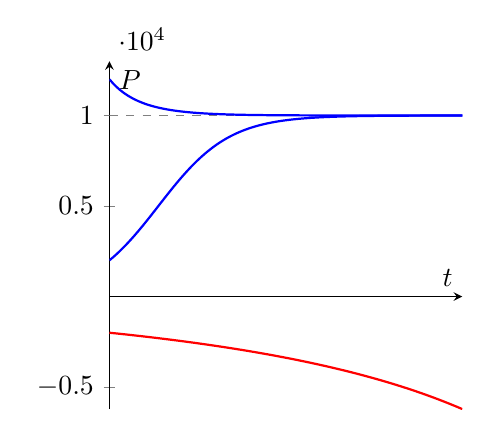
\begin{tikzpicture}
\begin{axis}[ 
height=6cm,
width=0.5\textwidth,
xlabel=$t$,
ylabel={$P$},
axis lines=middle,
xtick=\empty,
ymax=13000
] 
\addplot[gray,dashed,samples=50,domain=0:10] {10000};
\addplot[blue,samples=100,thick,domain=0:10] {2000*10000/(2000+(10000-2000)*e^(-x))};
\addplot[blue,samples=100,thick,domain=0:10] {12000*10000/(12000+(10000-12000)*e^(-x))};
\addplot[red,samples=100,thick,domain=0:10] {(-2000)*10000/(-2000+(10000+2000)*e^(-1/12*x))}; 
\end{axis}
\end{tikzpicture}
}{}
\end{floatrow}
\end{figure}

\paragraph{}

\begin{tcolorbox}{}

\[
\boxed{\od{x}{t}=f(x)} \to \text{ 1\textsuperscript{ης} τάξης, χρονικά αμετάβλητη}
\]
Σκοπός είναι να βρω την ποιοτική της συμπεριφορά με γραφική ανάλυση.
\end{tcolorbox}

\paragraph{Παρ.}
Να σχεδιαστούν οι λύσεις της ΔΕ \( \od{y}{t} = (y+1)(y-2) \) \quad (\(*\))

% {y[t] == (2 - 2 E^(3 t) + a (2 + E^(3 t)))/(1 + a + 2 E^(3 t) - a E^(3 t))}
\begin{figure}[h]\CenterFloatBoxes
\begin{floatrow}
\ffigbox[\FBwidth]{
	\parbox{0.4\textwidth}{
		\[
		y \quad\ -\infty \quad \quad -1 \quad 1/2 \qquad 2 \quad\ +\infty
		\]
		\[
		\begin{array}{r|c|c|c|c}
		y'(t) & + & - & - & + \\ \hline
		y''(t) & - & + & - & +  \\ \hline
		y(t) & \nearrow \cap & \searrow \cup & \searrow \cap & \nearrow \cup
		\end{array}
		\]
	}}{}
	\qquad
	\ffigbox[\FBwidth]{
		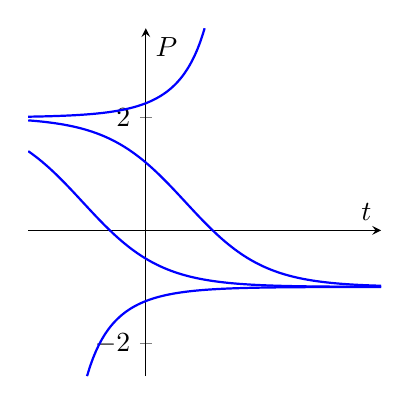
\begin{tikzpicture}
		\begin{axis}[ 
		height=6cm,
		width=0.5\textwidth,
		xlabel=$t$,
		ylabel={$P$},
		axis lines=middle,
		xtick=\empty%,
		%ymax=13000
		] 
		%\addplot[gray,dashed,samples=50,domain=0:10] {10000};
		\addplot[blue,samples=100,thick,domain=-1:0.5] {
			(2-2*e^(3*x) + 9/4 * (2+e^(3*x)) )/(1+ 9/4 + 2 *e^(3*x)-9/4*e^(3*x))
		};
		\addplot[blue,samples=100,thick,domain=-1:2] {
			(2-2*e^(3*x) + 1.2 * (2+e^(3*x)) )/(1+ 1.2 + 2 *e^(3*x)-1.2*e^(3*x))
		};
		\addplot[blue,samples=100,thick,domain=-1:2] {
			(2-2*e^(3*x) + -1/2 * (2+e^(3*x)) )/(1-1/2 + 2 *e^(3*x)+1/2*e^(3*x))
		};
		\addplot[blue,samples=100,thick,domain=-0.5:2] {
			(2-2*e^(3*x) + -2.5/2 * (2+e^(3*x)) )/(1-2.5/2 + 2 *e^(3*x)+2.5/2*e^(3*x))
		};
		\end{axis}
		\end{tikzpicture}
	}{}
	\end{floatrow}
	\end{figure}

Βλέπω ότι η (\(*\)) έχει 2 σημεία ισορροπίας. \\
Το \( y_1=-1 \) είναι \underline{ευσταθές} \\
Το \( y_2=2 \) είναι \underline{ασταθές}.

\paragraph{}

Η συνάρτηση \( \od{y}{t} = \sin y \) έχει πλάκα.

\subsection{}
\begin{tcolorbox}{Συστήματα}
\begin{align*}
\od{x}{t} &= f(x,y) \\
\od{y}{t} &= g(x,y)
\end{align*}
\end{tcolorbox}

\paragraph{π.χ.}
\begin{align*}
\od{x}{t} &= -y \\
\od{y}{t} &= x
\end{align*}

\begin{align*}
\frac{\dif x}{-y} = \dif t = \frac{\dif y }{x} \implies \\
x\dif x = -y\dif y \implies \\
x\dif x = y\dif y \implies \\
\frac{1}{2} \dif(x^2+y^2) = \dif c \implies \\
x^2+y^2=2c
\end{align*}

Σημεία ισορροπίας
\[
\left. \begin{array}{l}
\od{x}{t} = -y = 0 \\
\od{y}{t}=x=0
\end{array} \right| \implies (x_0,y_0) = (0,0)
\]

\begin{figure}[h]
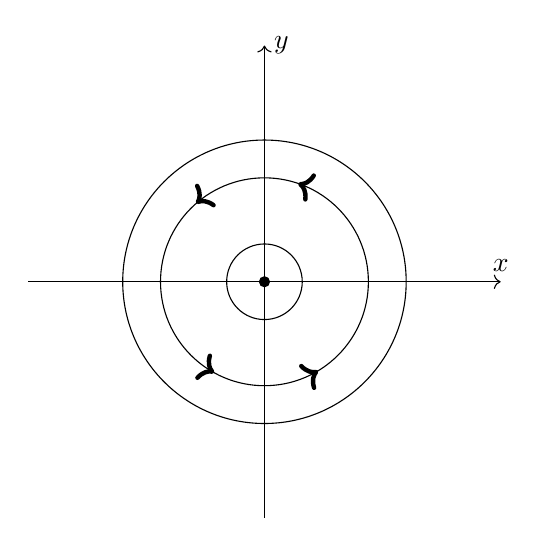
\begin{tikzpicture}[scale=0.6]
\draw[->] (-5,0) -- (5,0) node[anchor=east,above] {$x$};
\draw[->] (0,-5) -- (0,5) node[anchor=west] {$y$};
\draw (0,0) circle (3);
\draw (0,0) circle (2.2);
\draw (0,0) circle (0.8);
\draw[
decoration={markings,mark=at position 1 with {\arrow[ultra thick]{>}}},
postaction={decorate}
]
(70:2.2) -- (71:2.2); 
\draw[
decoration={markings,mark=at position 1 with {\arrow[ultra thick]{>}}},
postaction={decorate}
]
(130:2.2) -- (131:2.2); 
\draw[
decoration={markings,mark=at position 1 with {\arrow[ultra thick]{>}}},
postaction={decorate}
]
(240:2.2) -- (241:2.2); 
\draw[
decoration={markings,mark=at position 1 with {\arrow[ultra thick]{>}}},
postaction={decorate}
]
(-60:2.2) -- (-59:2.2); 
\filldraw[black] (0,0) circle (3pt);
\end{tikzpicture}
\end{figure}

\paragraph{Παρ.}
\begin{align*}
\od{x}{t} &= -x+y \\
\od{y}{t} &= -x-y
\end{align*}
\subparagraph{Σημεία ισορροπίας}
\[
\left. \begin{array}{l}
-x+y=0 \\
-x-y=0
\end{array} \right| \implies (x_0,y_0) = (0,0)
\]

\begin{align*}
\od{x}{y} = \frac{x-y}{x+y} \implies \cdots \implies \begin{cases}
x(t) &=e^{-t}\sin t \\
y(t) &= e^{-t} \cos t
\end{cases} \implies x^2+y^2=e^{-2t}
\end{align*}

\begin{figure}[h]
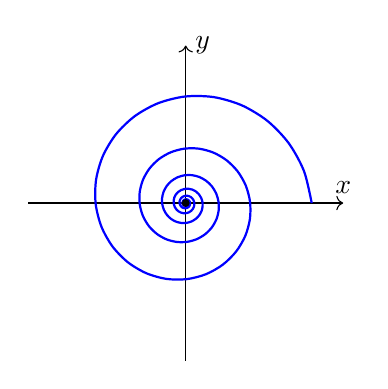
\begin{tikzpicture}[scale=0.4]
\draw[->] (-5,0) -- (5,0) node[anchor=east,above] {$x$};
\draw[->] (0,-5) -- (0,5) node[anchor=west] {$y$};
\draw [thick, color=blue, domain=0:25*pi, samples=300, smooth]
plot (xy polar cs:angle=\x r, radius={4*e^(-1/535*(\x r))});
\filldraw[black] (0,0) circle (3pt);
\end{tikzpicture}
Οι διάφορες λύσεις του συστήματος δε θα τέμνονται ποτέ! Γιατί?
\end{figure}


\paragraph{Παρ.}
\begin{align*}
\left. \begin{array}{ll}
\od{x}{t} &= xy \\
\pd{y}{t} &= x^2
\end{array} \right| &\implies \od{y}{x} = \frac{x}{y}
\\ &\implies x\dif x-y\dif y = 0
\\ &\implies x^2-y^2 =c
\end{align*}

Σημεία ισορροπίας
\begin{align*}
\left.
\begin{array}{ll}
xy &=0 \\ x^2 & = 0
\end{array} \right| \implies \text{ λύσεις } (0,A)
\end{align*}

Ευσταθή σημεία ισορροπίας είναι τα \( (x,y)=(0,A) \) με \( A \leq 0 \)

\begin{figure}[h]
\centering
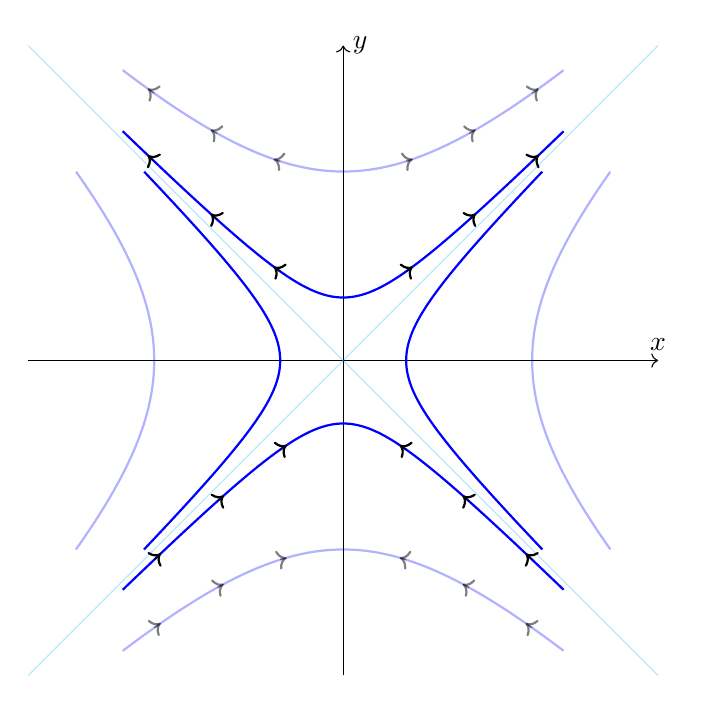
\begin{tikzpicture}[scale=0.8]
\draw[->] (-5,0) -- (5,0) node[anchor=east,above] {$x$};
\draw[->] (0,-5) -- (0,5) node[anchor=west] {$y$};
\draw [thick, color=blue, domain=-3:3,variable=\y, samples=200, smooth]
plot ({
	sqrt(\y*\y + 1)
},{\y});
\draw [thick, color=blue, domain=-3:3,variable=\y, samples=200, smooth]
plot ({
	-sqrt(\y*\y + 1)
},{\y});
\draw [thick, color=blue, domain=-3.5:3.5, samples=200, smooth]
plot ({\x},{
	sqrt(\x*\x + 1)
});
\draw [thick, color=blue, domain=-3.5:3.5, samples=200, smooth]
plot ({\x},{
	-sqrt(\x*\x + 1)
});


\draw [thick, opacity=0.3, color=blue, domain=-3:3,variable=\y, samples=200, smooth]
plot ({
	sqrt(\y*\y + 9)
},{\y});
\draw [thick, opacity=0.3, color=blue, domain=-3:3,variable=\y, samples=200, smooth]
plot ({
	-sqrt(\y*\y + 9)
},{\y});
\draw [thick, opacity=0.3, color=blue, domain=-3.5:3.5, samples=200, smooth]
plot ({\x},{
	sqrt(\x*\x + 9)
});
\draw [thick, opacity=0.3, color=blue, domain=-3.5:3.5, samples=200, smooth
]
plot ({\x},{
	-sqrt(\x*\x + 9)
});

\draw[thin, cyan, opacity=0.3] (-5,-5) -- (5,5);
\draw[thin, cyan, opacity=0.3] (5,-5) -- (-5,5);



\def\r{9}
\def\op{0.5}
\def\off{-0.1}
\foreach \x in {1,...,3}
\draw[
decoration={markings,mark=at position 1 with {\arrow[thick]{>}}},postaction={decorate},opacity=\op
](\x,{-sqrt(\x*\x+\r)}) -- (\x+\off,{-sqrt((\x+\off)*(\x+\off)+\r)}); 

\def\r{1}
\def\op{1}
\def\off{-0.1}
\foreach \x in {1,...,3}
\draw[
decoration={markings,mark=at position 1 with {\arrow[thick]{>}}},postaction={decorate},opacity=\op
](\x,{-sqrt(\x*\x+\r)}) -- (\x+\off,{-sqrt((\x+\off)*(\x+\off)+\r)}); 

\def\r{9}
\def\op{0.5}
\def\off{0.1}
\foreach \x in {1,...,3}
\draw[
decoration={markings,mark=at position 1 with {\arrow[thick]{>}}},postaction={decorate},opacity=\op
](\x,{sqrt(\x*\x+\r)}) -- (\x+\off,{sqrt((\x+\off)*(\x+\off)+\r)}); 

\def\r{1}
\def\op{1}
\def\off{0.1}
\foreach \x in {1,...,3}
\draw[
decoration={markings,mark=at position 1 with {\arrow[thick]{>}}},postaction={decorate},opacity=\op
](\x,{sqrt(\x*\x+\r)}) -- (\x+\off,{sqrt((\x+\off)*(\x+\off)+\r)}); 

\def\r{9}
\def\op{0.5}
\def\off{0.1}
\foreach \x in {1,...,3}
\draw[
decoration={markings,mark=at position 1 with {\arrow[thick]{>}}},postaction={decorate},opacity=\op
](-\x,{sqrt(\x*\x+\r)}) -- (-\x-\off,{sqrt((\x+\off)*(\x+\off)+\r)}); 

\def\r{1}
\def\op{1}
\def\off{0.1}
\foreach \x in {1,...,3}
\draw[
decoration={markings,mark=at position 1 with {\arrow[thick]{>}}},postaction={decorate},opacity=\op
](-\x,{sqrt(\x*\x+\r)}) -- (-\x-\off,{sqrt((\x+\off)*(\x+\off)+\r)}); 

\def\r{9}
\def\op{0.5}
\def\off{-0.1}
\foreach \x in {1,...,3}
\draw[
decoration={markings,mark=at position 1 with {\arrow[thick]{>}}},postaction={decorate},opacity=\op
](-\x,{-sqrt(\x*\x+\r)}) -- (-\x-\off,{-sqrt((\x+\off)*(\x+\off)+\r)}); 

\def\r{1}
\def\op{1}
\def\off{-0.1}
\foreach \x in {1,...,3}
\draw[
decoration={markings,mark=at position 1 with {\arrow[thick]{>}}},postaction={decorate},opacity=\op
](-\x,{-sqrt(\x*\x+\r)}) -- (-\x-\off,{-sqrt((\x+\off)*(\x+\off)+\r)}); 

\end{tikzpicture}
\end{figure}



\begin{exercise*}{}
\[
\od{x}{t} = x+y-x \cdot (x^2+y^2)
\]
\[
\od{y}{t} = -x+y-y\cdot(x^2+y^2)
\]
\tcblower
\begin{align*}
x\od{x}{t} &= x^2+xy - x^2\cdot (x^2+y^2) \\
y\od{y}{t} &= -xy+y^2-y^2\cdot(x^2+y^2) \\
\implies x\od{x}{t} + y\od{y}{t} &= x^2+y^2 - (x^2+y^2)\cdot(x^2+y^2) 
\intertext{Θέτω \( u=x^2+y^2 \)}
\od{u}{t} &= 2 \cdot \left(u -u^2\right) = 2 \cdot u \cdot (1-u)
\end{align*}

Για το \( u \) σημεία ισορροπίας
\[
\begin{cases}
u = 0 = x^2+y^2 \qquad & \text{ασταθές} \\
u = 1 = x^2+y^2 \qquad & \text{ευσταθές}
\end{cases}
\]

Άρα \( \forall (x,y) \neq (0,0):
\left.
\begin{array}{l}
x(0) = x_0 \\ y(0) = y_0
\end{array}
\right| \implies
x^2(t)+y^2(t) \rightarrow 1
 \)
 
 \( 
\left.
\begin{array}{l}
\od{x}{t} = x+y - x \cdot (x^2+y^2) \\
\od{y}{t} = -x+y-y\cdot (x^2+y^2)
\end{array}
 \right| \) όταν το \( t \rightarrow \infty \) γίνεται
  \( 
  \left.
  \begin{array}{l|r}
  \od{x}{t} \simeq& x+y - x =y \\
  \od{y}{t} \simeq& -x+y-y=-x
  \end{array}
  \right| 
  \implies \begin{array}{l}
  x(t) = A(t) \cos(t +\phi_0) \\ y(t) = A(t)\sin (t+\phi_0)
  \end{array}
  \)
  
  τ.ώ \( A(t) \to 1 \)
  
  %TODO phase plot for initial point inside circle & outside circle

\end{exercise*}

\begin{exercise*}{Το μοντέλο μάχης του \textlatin{Lancaster}}
\begin{align*}
\od{x}{t} &= -ay\mathrm h(x) \\
\od{y}{t} &= -bx\mathrm h(x)
\end{align*}
%TODO Plot h(x), h(0) = 0
\( x(0)=x_0 > 0 \)

\( y(0)=y_0 > 0 \)
\tcblower
%TODO phase plot
Σημεία ισορροπίας τα \( (0,A) A \geq 0,\ (B,0) B \geq 0 \)

Επίσης \( x(t) \downarrow,\ y(t) \downarrow \)

Αφού μένω πάντα στο 1ο 4ημόριο, ας εξετάσω την
\(  \left.
\begin{array}{l}
\od{x}{t}=-ay \\ \od{y}{t} = -bx
\end{array} \right| \implies \od{y}{x}=\frac{bx}{ay} \\ \implies ay\dif y -bx\dif x = 0 \implies
y^2(t)-x^2(t)=c=ay^2(0)-bx^2(0)
 \)
 
 Αν \( y(0) > \sqrt{\frac{b}{a}} x(0) \), νικάει ο \( Y \)


\end{exercise*}

\begin{exercise*}{Πρόβατα και κουνέλια}
\begin{align*}
\od{x}{t} &= (a-by)x \cdot \mathrm h(x) \\
\od{y}{t} &= (m-nx)y \cdot \mathrm h(x)
\end{align*}

\( x(0) = x_0, \ y(0) = y_0 >0,\ a,b,m,n>0 \)
\tcblower
%TODO 
%TODO phase plot with grace points
%TODO and different routes
%TODO 
\[
\left.
\begin{array}{ll}
\od{x}{t} &= (a-by)x \\ \od{y}{t} &= (m-nx)y
\end{array}
\right| \implies \frac{m-nx}{x} \dif x = \frac{a-by}{y} \dif y
\]

Έστω \( y < ^a/_b \implies \od{x}{t} > 0 \implies x(t) \uparrow \)

Έστω \( x < ^m/_n \implies \od{y}{t} > 0 \implies y(t) \uparrow \)


\end{exercise*}


\begin{exercise*}{Κουνέλια και αλεπούδες}
\begin{align*}
\od{x}{t} &= (a-by)\cdot x \\
\od{y}{t} &= (-m+nx)\cdot y
\end{align*}
Ίδιες συνθήκες
\tcblower
%TODO Phase Plot
\begin{align*}
y < \frac{a}{b} \implies x \uparrow \\
y > \frac{m}{n} \implies y \uparrow
\end{align*}
Ποτέ δε θα χτυπήσουμε πάνω στους απορροφητήρες.

\begin{align*}
& \frac{-m+nx}{x}\dif x = \frac{a-by}{y}\dif y \\
\implies & \frac{y^a}{e^{by}} = \kappa \cdot \frac{e^{nx}}{x^m}
\end{align*}
\end{exercise*}






\end{document}